\documentclass{iiufrgs}
\usepackage[latin1]{inputenc}
\usepackage{graphicx}
\usepackage[section]{placeins}
\usepackage{setspace}
\usepackage{fontenc}
\usepackage{listings}
\usepackage{color}
\usepackage{url}
\usepackage[printonlyused]{acronym}
\usepackage{rotating}
\usepackage{bytefield}
\usepackage[table]{xcolor}
\usepackage{multirow}
\usepackage{subfigure}
\usepackage{lscape}
\usepackage{enumitem}
\usepackage[toc,page]{appendix}

\onehalfspacing

\hyphenation{cmdStart}
\hyphenation{cmdPublishService}
\hyphenation{cmdSearchIdentifiers}
\hyphenation{cmdSearchService}
\hyphenation{cmdConnect}
\hyphenation{cmdSend}
\hyphenation{cmdReceive}
\hyphenation{CALVERT}
\hyphenation{BETTSTETTER}
\hyphenation{ARCINIEGAS}
\hyphenation{DEITEL}
\hyphenation{MICROSOFT}

\setdescription{topsep=1em,parsep=0pt,partopsep=0pt,itemsep=0pt}
\setitemize{topsep=1em,parsep=0pt,partopsep=0pt,itemsep=0pt}
\setenumerate{topsep=1em,parsep=0pt,partopsep=0pt,itemsep=0pt}

% Desenvolvimento da Ferramenta de Gerenciamento do Portal de Algoritmos da UCS
% Desenvolvimento de Ferramenta de Gerenciamento para o Portal de Algoritmos da UCS

\course{\cgcc}
\title{\\\large Evolu��o da Ferramenta de Gerenciamento do Portal de Algoritmos da UCS}
\author{Margarin}{Adriano}
\advisor[]{Nascimento}{Alexandre Erasmo Krohn}
\coadvisor[]{Dorneles}{Ricardo Vargas}
\location{Caxias do Sul}{}
\bibpunct{(}{)}{;}{a}{,}{,}

\def\lstlistlistingname{Lista de Trechos de C�digo}
\def\lstlistingname{Trecho de C�digo}
\definecolor{lightgray}{rgb}{0.95,0.95,0.95}
\definecolor{darkgray}{rgb}{0.3,0.3,0.3}
\lstset{
	language=Java,
	escapeinside={(*@}{@*)},
	basicstyle=\scriptsize\color{black}\ttfamily,
	numbers=left,
	numberstyle=\scriptsize\ttfamily,
	stepnumber=1,
	numbersep=5pt,
	tabsize=4,
	extendedchars=true,
	breaklines=true,
	frame=single,
	keywordstyle=\color{black}\textbf,
	keywordstyle=[1]\color{black}\textbf,
	keywordstyle=[2]\color{black}\textbf,
	keywordstyle=[3]\color{black}\textbf,
	keywordstyle=[4]\color{black}\textbf,
	stringstyle=\color{black}\ttfamily,
	showspaces=false,
	showtabs=false,
	xleftmargin=17pt,
	framextopmargin=4pt,
	framexleftmargin=20pt,
	framexrightmargin=5pt,
	framexbottommargin=4pt,
	backgroundcolor=\color{lightgray},
	showstringspaces=false
}

\newcommand{\bitformattingDefault}[1]{%
	\tiny
	\ifnum#1=6$\cdots$\else#1\fi
}
\newcommand{\colorbitbox}[3]{%
\rlap{\bitbox{#2}{\color{#1}\rule{\width}{\height}}}%
\bitbox{#2}{#3}}
\definecolor{colorPacote1}{rgb}{0.80,0.80,0.80}
\definecolor{colorPacote2}{rgb}{0.89,0.89,0.89}
\definecolor{colorPacote3}{rgb}{0.98,0.98,0.98}

\begin{document}

\maketitle

\begin{titlepage}
%\setcounter{page}{2} - Inclui o n�mero da p�gina
%\thispagestyle{headings}
\vfill

\begin{center}
{\setlength{\unitlength}{1cm}\makebox(12,6.5){\parbox[c]{12cm}{\setlength{\parskip}{0.8cm}\center\vskip -1.2cm\LARGE{\bf Evolu��o da Ferramenta de Gerenciamento do Portal de Algoritmos da Universidade de Caxias do Sul}\par \normalsize por\par \large Adriano Margarin\par}}}
\end{center}

{\large Trabalho de Conclus�o de Curso submetido ao curso de Bacharelado em Sistemas de Informa��o do Centro de Ci�ncias Exatas e da Tecnologia da Universidade de Caxias do Sul, como requisito obrigat�rio para gradua��o.}

\vfill

\begin{center}
{\Large\bf Trabalho de Conclus�o de Curso}
\end{center}

\vfill

\begin{singlespace}
Orientador: {Alexandre Erasmo Krohn Nascimento\par}
Coorientador: {Ricardo Vargas Dorneles\par}

Banca examinadora:\par
\hspace{1cm} {\setlength{\unitlength}{1cm}
\makebox(9,1){\parbox[c]{9cm}{\center Ricardo Vargas Dorneles\\ CCET/UCS}}}\par
\hspace{1cm} {\setlength{\unitlength}{1cm}
\makebox(9,1){\parbox[c]{9cm}{\center Andr� Luis Martinotto\\ CCET/UCS}}}\par

\vfill

\hfill{\setlength{\unitlength}{1cm}\makebox(9,2.5){\parbox[c]{9cm}{\setlength{\parskip}{0.8cm}\center\vskip -1.2cm Trabalho de Conclus�o de Curso apresentado em\\ 21 de Junho de 2018\par Andr� Gustavo Adami\\ Coordenador}}}

\end{singlespace}

\end{titlepage}

\begin{dedicatoria}
\sffamily\itshape
"A vida n�o � f�cil e ningu�m disse que seria."

\textsc{Henrique Bastos}
\end{dedicatoria}

\begin{agradecimentos}

Agrade�o a minha esposa, Marciele Luis, meus pais, Neusa Maria Margarin e Mauri Augusto Margarin, meus irm�os, Andr� Augusto Margarin e Let�cia Margarin pelo apoio no caminho trilhado at� aqui.

\vspace{20px}

A todos voc�s, minha sincera gratid�o.

\vspace{90px}

\hfill Adriano Margarin
\end{agradecimentos}

\tableofcontents

\chapter*{Lista de acr�nimos}

\vspace{20px}

\begin{acronym}[XXXXXXXXXX]
\acro{API}[\textit{API}]{\textit{Application Programming Interface}}
\acrodefplural{API}[\textit{APIs}]{\textit{Application Programming Interfaces}}
\acro{AVA}[\textit{AVA}]{\textit{Ambiente Virtual de Aprendizagem}}
\acro{CCET}[{CCET}]{Centro de Ci�ncias Exatas e da Tecnologia}
\acro{DAO}[{\textit{DAO}}]{\textit{Data Access Object}}
\acrodefplural{DAO}[{\textit{DAOs}}]{\textit{Data Access Object}}
\acro{HTML}[{\textit{HTML}}]{\textit{Hyper Text Markup Language}}
\acro{HTTP}[\textit{HTTP}]{\textit{Hyper Text Transfer Protocol}}
\acro{HTTPS}[\textit{HTTPS}]{\textit{Hyper Text Transfer Protocol Secure}}
\acro{SSL}[\textit{SSL}]{\textit{Secure Socket Layer}}
\acro{IHC}[{\textit{IHC}}]{Intera��o humano-computador}
\acro{JAR}[\textit{JAR}]{\textit{Java Archive}}
\acro{JAVA EE}[{\textit{JAVA EE}}]{\textit{Java Enterprise Edition}}
\acro{JDK}[\textit{JDK}]{\textit{Java Development Kit}}
\acro{MVC}[{\textit{MVC}}]{\textit{Model-View-Controller}}
\acro{NPAPI}[\textit{NPAPI}]{\textit{Netscape Plugin Application Programming Interface}}
\acro{ORM}[\textit{ORM}]{\textit{Object-relational mapping}}
\acro{REST}[\textit{REST}]{\textit{Representational State Transfer}}
\acro{SQL}[\textit{SQL}]{\textit{Structured Query Language}}
\acro{UCS}[{UCS}]{Universidade de Caxias do Sul}
\acro{UML}[\textit{UML}]{\textit{Unified Modeling Language}}
\acro{WWW}[{\textit{WWW}}]{\textit{World Wide Web}}
\acro{TCP}[{\textit{TCP}}]{\textit{Transmission Control Protocol}}
\acro{CSS}[{\textit{CSS}}]{\textit{Cascading Style Sheets}}
\acro{JDBC}[{\textit{JDBC}}]{\textit{Java Database Connectivity}}
\end{acronym}

\listoffigures
\listoftables

\begin{abstract}

Esse trabalho fornece todo o processo de evolu��o do portal de algoritmos. O trabalho tem por objetivo realizar a evolu��o do \textit{software} atual para uma vers�o mais moderna tecnologicamente e estruturalmente, para esse objetivo foram escolhidos tencologias atuais, como \textit{AngularJS}, \textit{Java 8}, \textit{Bootstrap 3}, \textit{Postgreslq 10}. Para atingirmos o objetivo utilizamos engenharia reversa, diagramas de casos de uso, diagrama de robustez, \textit{mockups} de interfaces gr�ficas e escolhemos a arquitetura \ac{MVC} para guiar no desenvolvimento. 

\keyword{Portal de Algoritmos}
\keyword{Algoritmos}
\keyword{Evolu��o}
\keyword{Software}

\end{abstract}

\acresetall

\chapter{Introdu��o}\label{cpIntroducao}

No presente trabalho foi realizada a evolu��o do m�dulo de gerenciamento do portal de algoritmos da Universidade de Caxias do Sul. No ano de 2016 foi concluido pelo aluno Gabriel Weber um trabalho que evoluiu o analisador algor�tmico \cite{Weber2015}.

O portal de algoritmos, desenvolvido no ano de 2009 pelos professores Ricardo Vargas Dorneles e Delcino Picinin Junior, da Universidade de Caxias do Sul, tem por objetivo auxiliar no ensino da l�gica de programa��o atrav�s da linguagem do portugu�s estruturado, tamb�m conhecida como portugol e � utilizado pelos alunos da �rea de Conhecimento de Ci�ncias Exatas e Engenharias e p�blico em geral. Esse portal oferece ao aluno a possibilidade de exercitar sua l�gica atrav�s de exerc�cios cadastrados pelos professores, utilizando a linguagem portugol em um editor espec�fico. O aluno submete solu��es de problemas a fim de valid�-las e pode acompanhar seu desempenho atrav�s de um ranking de submiss�es de solu��es corretas. O portal possui uma se��o de gerenciamento que somente administradores podem acessar. Nessa administra��o h� a possibilidade de acompanhar a evolu��o dos alunos, suas submiss�es de solu��es, visualiza��o e edi��o de usu�rio, de problemas, de dados de testes e palavras-chave \cite{Dorneles2004}.

No ano de 2016 o \textit{software} cliente do portal de algor�tmos foi refeito, pois naquele ano foi preciso migrar o programa escrito em \textit{Java Applet} para um aplicativo \textit{Desktop}, esse \textit{software Desktop} � instalado localmente e consumindo o \textit{Web Services} do portal de algor�tmos antigo. No entanto, o \textit{software} servidor n�o foi migrado, e � neste contexto que este trabalho est� inserido.

Na cria��o de um problema, o administrador informa um nome e uma descri��o do problema a ser solucionado, dicas e palavras-chave, sendo que as �ltimas  informa��es n�o s�o obrigat�rias. Tamb�m s�o informadas entradas de dados para testes e as sa�das esperadas para as entradas informadas. J� na edi��o do problema, as mesmas informa��es citadas acimas podem ser alteradas.

No m�dulo de administra��o � poss�vel manter todas as informa��es dos usu�rios, problemas, palavras-chave, dados de testes, dentre outras informa��es.

Devido � constante evolu��o tecnol�gica, o portal de algoritmos ficou defasado, com problemas de compatibilidade com os navegadores atuais e pouca ou nenhuma seguran�a. Funcionalidades limitadas no seu gerenciamento tamb�m foram apontadas pelos usu�rios como alvo de melhorias.

As tecnologias utilizadas no desenvolvimento do portal atual, \textit{Python } vers�o 2.6, \textit{Django} vers�o 1.2, \textit{Plugins} \ac{NPAPI} (\textit{Java Applet}), est�o desatualizadas e/ou foram descontinuadas. No caso da tecnologia \ac{NPAPI}, esta foi totalmente desativada \cite{Python2015, Django2015, NPAPI2015}.

Um dos problemas citados acima s�o as vers�es do \textit{Python} e \textit{Django}, que est�o em vers�es desatualizadas e sem suporte t�cnico por seus desenvolvedores.

O editor de solu��es do portal atual foi programado como sendo um \textit{Applet Java}. \textit{Applets} executam nos navegadores, utilizando a tecnologia de plugins \textit{NPAPI} \cite{NPAPI2015}. \textit{Plugins} \ac{NPAPI} deixaram de ser suportados pelos navegadores atuais, pelo fato de causarem riscos de seguran�a para quem esteja utilizando. Desde o dia 1� de Setembro de 2015, o navegador \textit{Google Chrome} deixou de suportar todas as tecnologias que utilizam \ac{NPAPI}, como \textit{Flash}, \textit{Java}, entre outros. Mesmo eles n�o sendo mais suportados nativamente, � poss�vel ativar isso no navegador, mas isso pode causar vunerabilidades para quem deseja fazer isto \cite{NPAPI2015}.

Para resolver os problems citados acima, este trabalho visa realizar a engenharia reversa do aplicativo, da modelagem de banco de dados atual, reengenharia de \textit{software} e evolu��o de \textit{software} atrav�s de t�cnicas de engenharia de \textit{software} e desenvolvimento.

Atrav�s da engenharia reversa, o programa � analisado e s�o extra�das as informa��es, facilitando a documenta��o de sua organiza��o e funcionalidades \cite{Sommerville2011}.

Para realizar a engenharia reversa � preciso fazer a tradu��o de seu c�digo fonte, sendo que o atual \textit{software} foi desenvolvido utilizando a linguagem de programa��o \textit{Python} e o \textit{Django} \cite{Django2015}.

Com \textit{Python} e \textit{Django} foram desenvolvidas todos os modelos de classes de dom�nio, que ser�o detalhadas no Cap�tulo \ref{cpReengenhariaSoftware}, usando o \ac{ORM} do \textit{Django} foram criadas as tabelas de banco de dados e s�o realizadas as consultas. 

Ser� realizada a diagrama��o das classes atuais utilizando-se da nota��o \ac{UML}. Ser�o utilizados diagramas de classes de dom�nio, que representar�o essas classes, interfaces e suas associa��es, para que depois sejam usadas no desenvolvimento de um modelo de sistema orientado a objetos \cite{Pressman2011, Sommerville2011}.

Atrav�s da engenharia de \textit{software} ser� produzido um novo portal de algoritmos, desde os est�gios inicias da especifica��o do sistema at� sua implementa��o e instala��o. Com o uso de engenharia de \textit{software} espera-se obter resultados de qualidade e requeridos dentro do cronograma \cite{Sommerville2011}.

Para atingir o objetivo proposto, o trabalho est� organizado da seguinte forma:

No Cap�tulo \ref{cpReferencial} s�o apresentados todos os conceitos metodol�gicos da engenharia de \textit{software}, quais tecnologias que ser�o utilizadas e suas fun��es no contexto do trabalho.

No Cap�tulo \ref{cpReengenhariaSoftware} � apresentada a reengenharia de \textit{software} realizada no portal de algoritmos atual.

No Cap�tulo \ref{cpProposta} � apresentada a modelagem para a evolu��o do \textit{software}, suas interfaces e diagramas relacionados.

No Cap�tulo \ref{seguranca} � apresentado uma proposta de seguran�a para o servidor, essa seguran�a deve ser configurada na infra-estrutura.

No Cap�tulo \ref{cpConsideracoesParciais} s�o apresentadas as considera��es finais do trabalho.

\chapter{Evolu��o de Software}\label{cpReferencial}

Para manter um \textit{software} �til ele deve mudar continuamente. Essa mudan�a pode ser a partir de uma press�o constante de mudan�as que os usu�rios imp�em, para facilitar ou automatizar algumas tarefas do dia-a-dia, entre outros fatores.

Todos os \textit{softwares} passar�o pelo processo de envelhecimento, isso � inevit�vel. Algumas causas de problemas podem ser previstas, minimizando os impactos dos danos que s�o causados por esse fator. A continuidade de uso do \textit{software} implica que ocorram mudan�as, que podem ocorrer em regras de neg�cio ou nas expectativas dos usu�rios \cite{Sommerville2011}.

\citet{Rezende2005}, define que um \textit{software} tem um ciclo de vida de no m�ximo 10 anos, quando ele n�o sofre novas implementa��es. O ciclo de vida natural de um \textit{software} abrange as seguintes fases: concep��o, constru��o, implementa��es, implanta��o, maturidade e utiliza��o plena, decl�nio, manuten��o e morte.

Devido a esse ciclo de vida, uma evolu��o de \textit{software} pode ser desencadeada por necessidades de novos componentes, por defeitos relatados ou devido a mudan�as de outros sistemas \cite{Sommerville2011}.

A evolu��o de \textit{software} compreende as mudan�as que ir�o ocorrer a fim de deix�-lo completo e, se poss�vel, livre de erros \cite{Sommerville2011}. Mas para essa evolu��o acontecer � necess�rio considerar diversos fatores que servir�o de base para que um novo software seja constru�do, com base nos requisitos do atual.

O processo de evolu��o varia conforme o tipo de \textit{software} que esteja sendo mantido, dos processos de desenvolvimento e as habilidades das pessoas envolvidas. Em alguns casos a evolu��o pode ser um processo informal, em que na maioria das vezes as mudan�as resultam de conversas com usu�rios. J� em outros casos � um processo formal, envolvendo documenta��o estruturada que � produzida em cada est�gio do processo \cite{Sommerville2011}.

O processo de evolu��o de \textit{software} envolve a compreens�o do \textit{software} que tem que ser alterado. Para tornar-se poss�vel a evolu��o � preciso aplicar reengenharia no \textit{software} atual, visando melhorar sua estrutura e inteligibilidade \cite{Sommerville2011}.

Para tornar poss�vel a evolu��o de \textit{software} � preciso seguir alguns processos. Nas pr�ximas se��es ser�o apresentadas as metodologias e tecnologias que ser�o utilizadas neste trabalho.

\begin{itemize}
	\item Reengenharia de \textit{Software}
	\item Engenharia Reversa
	\item Engenharia de \textit{Software}
	\item Processo de \textit{Software}
	\item Engenharia de Requisitos
	\item Casos de Uso
	\item Modelagem de Dom�nio
	\item Metodologia ICONIX
	\item Projeto de Arquitetura
	\item Usabilidade
	\item Tecnologias
		\begin{itemize}
			\item Python e Django
			\item Java EE
			\item Wildfly
			\item DAO
			\item \ac{REST}
			\item AngularJS
		\end{itemize}
\end{itemize}

\section{Reengenharia de Software}

A reengenharia de \textit{software} pode envolver a redocumenta��o do sistema, a refatora��o da arquitetura, a mudan�a de linguagem de programa��o para uma liguagem mais moderna e modifica��es e atualiza��o de estrutura e dos dados de sistema. A funcionalidade n�o � alterada, e geralmente deve evitar grandes mudan�as na arquitetura \cite{Sommerville2011}.

Alguns benef�cios importantes na reengenharia � o risco reduzido quando trata-se de um \textit{software} cr�tico de neg�cio, onde podem haver erros nas especifica��es e atrasos no in�cio do novo, e o custo reduzido, onde o custo da reengenharia se torna significamente menor do que o desenvolvimento de um novo.

A Figura \ref{imgReengenhariaSoftware} demonstra o processo geral da reengenharia, onde a entrada � um sistema legado e a sa�da � uma vers�o melhorada do mesmo.

\FloatBarrier
\begin{figure}[!htb]
	\centering
	\caption{Processo de Reengenharia}
	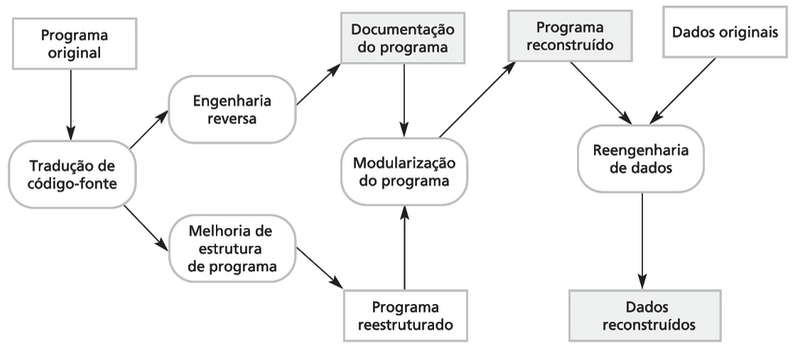
\includegraphics[width=15cm]{imagens/processo-reengenharia.png}
	\label{imgReengenhariaSoftware}
	Fonte: \cite{Sommerville2011}
\end{figure}
\FloatBarrier

\begin{enumerate}
	\item Tradu��o de c�digo-fonte: atrav�s de alguma ferramenta de tradu��o, o programa � convertido para uma vers�o mais atual da linguagem ou para outra diferente.
	\item Engenharia reversa: o programa � analisado e as informa��es s�o extra�das a partir dele.
	\item Melhoria na estrutura de programa: a estrutura de controle � analisada e modificada para que se torne mais f�cil de ler e entender.
	\item Modulariza��o de programa: partes relacionadas do programa s�o agrupadas, e onde houver redund�ncia, se apropriado, esta � removida. Em alguns casos, esse est�gio pode envolver refatora��o de arquitetura.
	\item Reengenharia dos dados: os dados processados pelo programa s�o alterados para refletir as mudan�as de programa.
\end{enumerate}

Nem sempre � necess�rio seguir todas as etapas da Figura \ref{imgReengenhariaSoftware}. Pode haver casos em que se utiliza o mesmo ambiente de desenvolvimento da linguagem de programa��o. Nesse caso n�o � necess�rio a tradu��o do c�digo \cite{Sommerville2011}.

Na reengenharia um dos processos � a engenharia reversa. Na pr�xima se��o � descrito como ela � utilizada no processo de evolu��o.

\section{Engenharia Reversa}

A engenharia reversa, segundo \citet{Sommerville2011}, consiste em uma t�cnica de an�lise de software com o objetivo de recuperar o projeto e suas especifica��es t�cnicas.

� poss�vel fazer a engenharia reversa atrav�s de diversas formas, na maioria das vezes utiliza os de c�digos fontes, conhecimentos t�cnicos e experi�ncias dos pr�prios desenvolvedores.

Na se��o seguinte � descrita a Engenharia de \textit{software} e suas respectivas camadas.

\section{Engenharia de Software}

Engenharia de \textit{software} � uma disciplina cujo foco est� em todos os aspectos da produ��o de software, partindo dos est�gios iniciais da especifica��o do \textit{software} at� sua manuten��o, quando o \textit{software} j� est� em funcionamento \cite{Sommerville2011}. De acordo com \citet{Rezende2005}, ``� a metodologia de desenvolvimento e manuten��o de sistemas modulares, com as as seguintes caracter�sticas: processo din�mico, integrado e inteligente de solu��es tecnol�gicas; adequa��o aos requisitos funcionais do neg�cio do cliente e seus respectivos procedimentos pertinentes; efetiva��o de padr�es de qualidade, produtividade e efetividade em suas atividades e produtos; fundamenta��o da Tecnologia da Informa��o dispon�vel, vi�vel, oportuna e personalizada; planejamento e gest�o de atividades, recursos, custos e datas".

Conforme podemos ver na Figura \ref{imgCamadasEngenhariaSoftware}, a engenharia de \textit{software} � uma tecnologia em camadas. A base para a engenharia de \textit{software} � a camada de processos. O processo de engenharia de \textit{software} � o m�todo que permite manter as camadas de tecnologia coesa e possibilita o desenvolvimento do \textit{software} \cite{Pressman2011}.

\FloatBarrier
\begin{figure}[!htb]
	\centering
	\caption{Camadas da Engenharia de Software}
	
\includegraphics[width=15cm]{imagens/camadas-engenharia-de-software.png}
	\label{imgCamadasEngenhariaSoftware}
	Fonte: \cite{Pressman2011}
\end{figure}
\FloatBarrier

A engenharia de \textit{software} � realizada atrav�s de processos de \textit{software}, que ser�o descritos a seguir.

\section{Processo de Software}

Um processo de \textit{software} � um conjunto de atividades, a��es e tarefas relacionadas que levam � produ��o de um produto de \textit{software} \cite{Sommerville2011, Pressman2011}. No contexto da engenharia de \textit{software}, um processo n�o � uma prescri��o r�gida de como desenvolver, ele � adapt�vel, que possibilita �s pessoas realizar o trabalho de selecionar e escolher o conjunto apropriado de a��es e tarefas \cite{Pressman2011}.

Dentre muitos processos de \textit{software} existentes todos devem incluir quatro atividades fundamentais \cite{Sommerville2011}.

\begin{itemize}
	\item Especifica��o de \textit{software}
	\item Projeto e implementa��o de \textit{software}
	\item Valida��o de \textit{software}
	\item Evolu��o de \textit{software}
\end{itemize}

De acordo com \citet{Sommerville2011}, essas atividades fazem parte do processo de \textit{software}. Na pr�tica eles s�o complexos, possuem subatividades, entre elas levantamento de requisitos, projeto de arquitetura, testes etc.

Para melhor entendimento desses processos, nas pr�ximas se��es ser�o descritas com mais detalhes algumas dessas atividades.

\section{Engenharia de Requisitos}

Engenharia de requisitos de sistemas basicamente � o conjunto das descri��es do que o sistema deve fazer, o que ele oferece de servi�o e restri��es a seu funcionamento \citet{Sommerville2011}. A engenharia de requisitos abrange sete tarefas distintas: concep��o, levantamento, elabora��o, negocia��o, especifica��o, valida��o e gest�o, onde geralmente algumas ocorrem em paralelo e todas podem ser adaptadas � necessidade de cada projeto \cite{Pressman2011}

Somente descrever os requisitos n�o � suficiente, � preciso entender o que est� descrito, e essa � uma das tarefas mais dif�ceis enfrentadas por um engenheiro de \textit{software}.

Os requisitos de \textit{software} frequentemente s�o classificados em funcionais e n�o-funcionais.

Requisitos funcionais s�o declara��es de servi�o que o sistema deve fornecer, de como fornecer, de como o sistema deve reagir a entradas espec�ficas e de como o sistema deve se comportar em determinadas sistua��es. Em alguns casos, os requisitos funcionais tamb�m podem explicitar o que o sistema n�o deve fazer \cite{Sommerville2011}.

Requisitos n�o-funcionais s�o restri��es aos servi�os ou fun��es oferecidas pelo sistema. Incluem restri��es de \textit{timing}, restri��es no processo de desenvolvimento e restri��es impostas pelas normas. Ao contr�rio das caracter�sticas individuais ou servi�os do sistema, os requisitos n�o funcionais muitas vezes aplicam-se ao sistema como um todo \cite{Sommerville2011}.

\section{Casos de Uso}

Casos de uso tem por objetivo descrever os requisitos funcionais, delimita��o do contexto do sistema documentado e entendimento dos requisitos, onde cada caso de uso deve descrever somente uma funcionalidade ou objetivo do sistema \cite{Sommerville2011} e \cite{Pressman2011}.

Um conjunto de casos de uso representa todas as poss�veis intera��es que s�o descritas nos requisitos de sistema. Os atores podem ser pessoas ou outros sistemas e s�o representados como figuras ``palitos" \ e cadas classe de intera��o � representada por uma elipse \cite{Sommerville2011}.

Casos de uso possuem atores e cen�rios, onde os atores podem ser pessoas ou outros sistemas que interagem entre si, e os cen�rios s�o sequ�ncias espec�ficas de a��es. Em outros termos casos de uso � uma cole��o de cen�rios relacionados ao sucesso ou fracasso \cite{Larman2007}.

A Figura \ref{imgCasoUso} apresenta um exemplo de caso de uso de um consult�rio m�dico, onde podemos observar todos os atores envolvidos e suas respectivas a��es.

\FloatBarrier
\begin{figure}[!htb]
	\centering
	\caption{Casos de uso}
	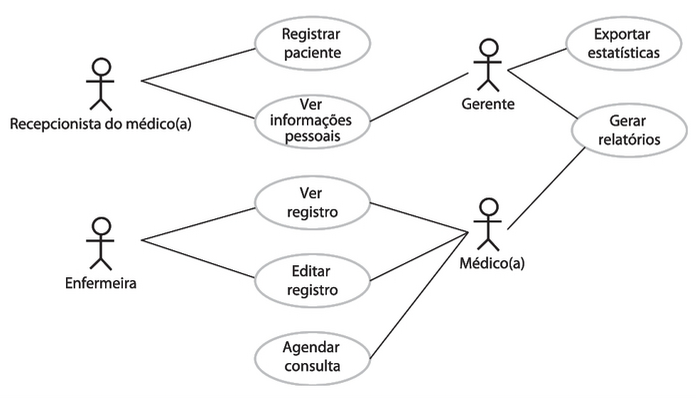
\includegraphics[width=15cm]{imagens/caso-de-uso.png}
	\label{imgCasoUso}
	Fonte: \cite{Sommerville2011}
\end{figure}
\FloatBarrier

A modelagem de caso de uso � um apoiador para a elicita��o de requisitos, geralmente descreve o que o usu�rio espera do sistema. Cada caso de uso representa uma tarefa que envolve a intera��o externa com o sistema \cite{Sommerville2011}.

\section{Metodologia ICONIX}

Para desenvolver um projeto, � necess�rio uma metodologia. Nesse trabalho, ser� utilizada a metodologia ICONIX.

A metodologia ICONIX foi elaborada por Doug Rosenberg e Kendal Scott, a partir de um processo simples e unificado dos pesquisadores Booch, Rumbaugh e Jacobson \cite{Rosenberg2005}.

As vantagens de se utilizar a metodologia ICONIX s�o: metodologia pr�tica, simples, espec�fica de forma objetiva e possui rastreabilidade dos requisitos \cite{Rosenberg2005}.

A metodologia ICONIX utiliza-se de um subconjunto da \ac{UML} no qual apenas 4 diagramas s�o utilizados: diagramas de classe, diagrama de sequ�ncia, diagrama de robustez e caso de usos \cite{Rosenberg2005}.

\subsection{Diagramas de Classe}

Os diagramas de classes s�o usados no desenvolvimento de um modelo de sistema orientado a objetos para mostrar as classes de um sistema e as associa��es entre essas classes \cite{Sommerville2011}.

A Figura \ref{imgExDiagramaClasse} indica as rela��es entre os objetos da classe Paciente e objetos de outras classes \cite{Sommerville2011}.

\FloatBarrier
\begin{figure}[!htb]
	\centering
	\caption{Diagramas de Classe}
	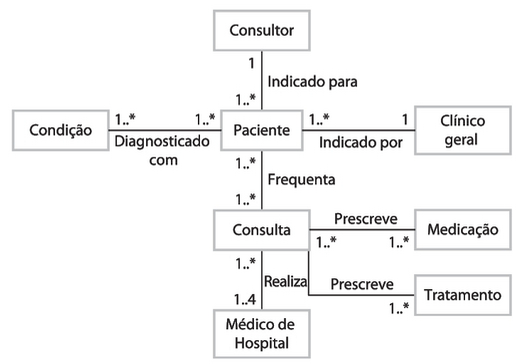
\includegraphics[width=13cm]{imagens/exemplo-diagrama-de-classe.png}
	\label{imgExDiagramaClasse}
	\newline
	Fonte: \cite{Sommerville2011}
\end{figure}
\FloatBarrier

\subsection{Diagrama de Sequ�ncia}

Os diagramas de sequ�ncia geralmente s�o utilizados para modelar as intera��es entre os atores e os objetos em um sistema \cite{Sommerville2011}.

\FloatBarrier
\begin{figure}[!htb]
	\centering
	\caption{Diagrama de Sequ�ncia}
	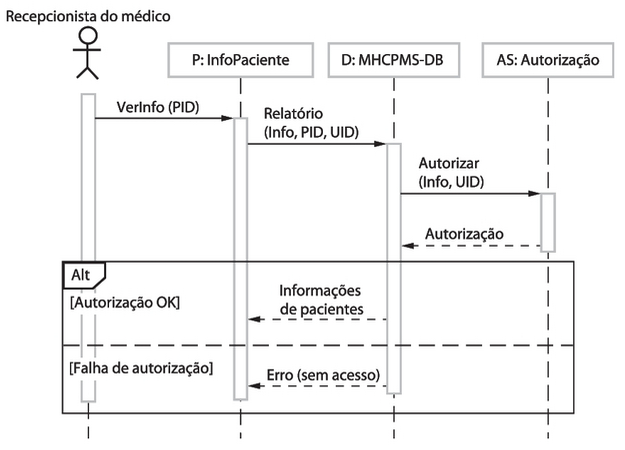
\includegraphics[width=15cm]{imagens/exemplo-diagrama-sequencia.png}
	\label{imgExSequencia}
	Fonte: \cite{Sommerville2011}
\end{figure}
\FloatBarrier

A Figura \ref{imgExSequencia} pode ser lida da seguinte maneira:

\begin{enumerate}
	\item A recepcionista do m�dico aciona o m�todo VerInfo em uma inst�ncia P da classe de objeto InfoPaciente, fornecendo o identificador do paciente (PID, do ingl�s \textit{patient's identifier}). A inst�ncia P � um objeto de interface  do usu�rio, exibido como um formul�rio  que mostra os dados do paciente.
	\item A inst�ncia P chama o banco de dados para retornar as informa��es necess�rias, fornecendo o identificador da recepcionista, que permite a verifica��o de prote��o (nessa fase, n�o importa de onde vem o esse UID - do ingl�s, \textit{user's identifier}).
	\item O banco de dados verifica, com o sistema de autoriza��o, que o usu�rio est� autorizado a essa a��o.
	\item Se autorizado, as informa��es de pacientes s�o retornadas, e um formul�rio � preenchido na tela do usu�rio. Se falhar a autoriza��o, aparece uma mensagem de erro.
\end{enumerate}

\subsection{Diagrama de Robustez}

A Figura \ref{imgExRobustez} representa a intera��o entre o usu�rio e as interface de um sistema, bem como todas as intera��es entre as interfaces.

Como podemos observar na Figura \ref{imgExRobustez}, o ator usu�rio clica no ``�cone de contatos" na tela principal, ap�s o clique � exibido a tela de contatos, na sequ�ncia o ator clica em ``adicionar novo" no qual resulta na exibi��o da tela de novo contato, continuando a a��o o ator preenche os campos selecionados e faz a a��o de salvar contato na mem�ria retornando assim para para tela de exibi��o de contatos.

\FloatBarrier
\begin{figure}[!htb]
	\centering
	\caption{Diagrama e Robustez}
	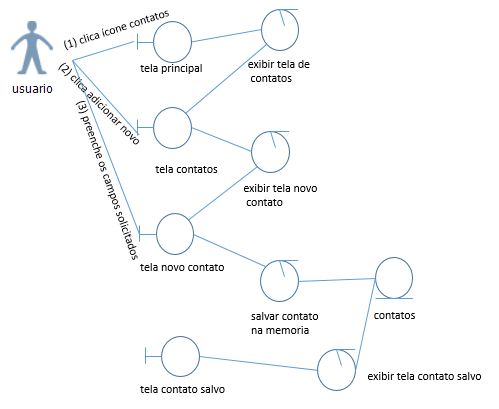
\includegraphics[width=10cm]{imagens/exemplo-diagrama-robustez.png}
	\label{imgExRobustez}
	\newline
	Fonte: \cite{Galeote2015}
\end{figure}
\FloatBarrier

\subsection{Casos de Usos}

A Figura \ref{imgExCasoUso} representa o caso de uso de transfer�ncia de dados que envolve os atores Recepcionista do m�dico e Sistema de registro de pacientes \cite{Sommerville2011}.

Como podemos observar na Figura \ref{imgExCasoUso} a recepcionista do m�dico realiza a transfer�ncia de dados para o sistema de registro de pacientes.

\FloatBarrier
\begin{figure}[!htb]
	\centering
	\caption{Casos de uso de transfer�ncia de dados}
	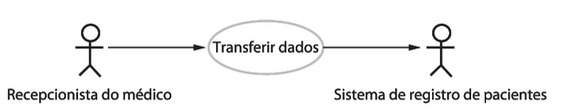
\includegraphics[width=13cm]{imagens/exemplo-caso-de-uso.png}
	\label{imgExCasoUso}
	\newline
	Fonte: \cite{Sommerville2011}
\end{figure}
\FloatBarrier

\section{Modelos de Dom�nio}

Um modelo de dom�nio exibe como est� organizado o sistema em termos de seus componentes e seus relacionamentos. Podem ser est�ticos ou din�micos, onde os modelos est�ticos mostram a estrutura do sistema e os din�micos, onde � exibido quando ele est� em execu��o \cite{Sommerville2011}.

De acordo com \citet{Sommerville2011}, ``os diagramas de classe s�o utilizados no desenvolvimento de um modelo de sistema orientado a objetos para mostrar as classes de um sistema e as associa��es entre essas classes".

Um modelo de dom�nio � uma representa��o visual de classes conceituais, ou objetos do mundo real, em um dom�nio \cite{Larman2007}. Tamb�m s�o conhecidos como modelos conceituais.

\section{Projeto de Arquitetura}

O projeto de arquitetura � a representa��o da estrutura de dados e seus componentes. Ele compreende como o sistema deve ser organizado a fim de atender as necessidades levantadas na engenharia de requisitos \cite{Sommerville2011, Pressman2011}.

Na arquitetura em camadas o \textit{software} � dividido em camadas, onde cada camada possui um pr�posito bem definido e cada camada conhece apenas a camada imediatamente inferior \cite{Sommerville2011}.

Na arquitetura em camadas encontram-se todas as camadas do \textit{software}, e define-se a responsabilidade de cada uma. Esse padr�o de arquitetura � uma das maneiras de se conseguir independ�ncia entre elas, como por exemplo o padr�o \ac{MVC}, em que s�o separadas as camadas de apresenta��o da intera��o dos dados do sistema \cite{Sommerville2011, Pressman2011}.

\section{Usabilidade}

Sistemas deve ser flex�veis, simples e agrad�veis de usar. A usabilidade � a principal busca da \ac{IHC}, \ac{IHC} tem por objetivo produzir sistemas us�veis, seguros e funcionais.

Na \ac{IHC}, a usabilidade se refere � simplicidade e facilidade com que uma interface de um sistema pode ser utilizado. A import�ncia do \ac{IHC} no desenvolvimento de \textit{software} � de ter uma defini��o de padr�o visual, padr�o de mensagens e prototipa��o e valida��o de telas com usu�rio, medindo a usabilidade e garantindo a padroniza��o e consist�ncia.

De acordo com \citet{Benyon2011}, um sistema com usabilidade ter� as seguintes caracter�sticas:

\begin{itemize}
	\item Ser� eficiente no sentido de que as pessoas poder�o fazer as coisas mediante uma quantidade adequada de esfor�o.
	\item Ser� eficaz no sentido de que conter� as fun��es e o conte�do de informa��es adequadas e organizadas de forma apropriada.
	\item Ser� f�cil aprender como fazer as coisas e ser� f�cil de lembrar como faz�-las ap�s algum tempo.
	\item Ser� seguro de operar na variedade de contextos em que ser� usado.
	\item Ter� um alto grau de utilidade no sentido de que far� as coisas que as pessoas querem que sejam feitas.
\end{itemize}

O portal de algoritmos atual apresenta algumas telas confusas, que podem ser observadas no Cap�tulo \ref{cpProposta} na Se��o \ref{scPrototipos}. Esse trabalho pretende melhor�-las.

At� aqui foram apresentadas as metodologias que ser�o utilizadas na evolu��o do aplicativo. Na se��o seguinte ser�o apresentadas as tecnologias escolhidas para a evolu��o do gerenciamento do portal de algoritmos.

\section{Tecnologias}

Nesta se��o ser�o descritas as tecnologias que v�o ser utilizadas na evolu��o do portal de algoritmos, tais como a linguagem de programa��o \textit{Java}, \ac{REST} e \textit{AngularJS}. S�o tecnologias bem consolidades no mercado, com \textit{upgrade} garantido por tempo indeterminado, mantidas por empresas s�rias e de grande porte.

\subsection{Python e Django}

O \textit{Python} � uma linguagem interpretada de alto n�vel, criada por Guido Van Rossum em 1989 e lan�ada em 1991 e atualmente possui o modelo de desenvolvimento comunit�rio \cite{Python2015}. Com o aux�lio do \textit{framework Django}, criado originalmente para gerenciar conte�dos de um jornal da cidade de Lawrence, no Kansas, � poss�vel definir a modelagem de dados atrav�s de classes \textit{Python} e gerar tabelas do banco de dados para manipula��o sem a necessidade de \ac{SQL} \cite{Django2015}.

\subsection{Java EE}

A linguagem Java � uma linguagem de programa��o orientada a objetos, com portabilidade, independ�ncia de plataforma, extensas bibliotecas de rotinas que facilitam recursos de rede e seguran�a, podendo executar programas via rede com restri��es de execu��es \cite{Java2015}.

Al�m disso, ela se destaca com a similaridade de sintaxe da linguagem C/C++, facilidade de internacionaliza��o, simplicidade nas especifica��es, entre outras \cite{Java2015}.

O \ac{JAVA EE} � uma s�rie de especifica��es que descrevem como deve ser implementado um \textit{software} que faz uso de servi�os de infraestrutura. Tamb�m � considerado uma maneira de desenvolver aplicativos com suporte a escabilidade, flexibilidade e seguran�a \cite{Java2015}.

\subsection{WildFly}

O servidor de aplica��o \textit{WildFly} implementa a mais recente vers�o do \ac{JAVA EE}, sendo mantido pela \textit{Red Hat} \cite{Wildfly2015}.

Os \textit{frameworks} que comp�em o \ac{JAVA EE} s�o fortemente testado em diversas combina��es. De acordo com padr�es com os quais o servidor foi desenvolvido o desenvolvedor pode focar nas regras de neg�cio e utilizar-se dos recursos de infraestrutura fornecidas pelo \textit{framework} \cite{Wildfly2015}.

\subsection{DAO}

\ac{DAO} � um mecanismo de acesso para trabalhar com fonte de dados, essa fonte de dados pode ser um banco de dados relacional, banco de dados orientado a objetos entre outros \cite{Deepak2004}.

Com \ac{DAO} � poss�vel adaptar a diferentes esquemas de armazenamento sem afetar outros componentes de neg�cio, basicamente o \ac{DAO} atua como um adaptador entre o componente e a fonte de dados \cite{Deepak2004}.

\subsection{REST}

O \ac{REST} n�o � um protocolo, � um formato de arquivo ou uma estrutura de desenvolvimento. \ac{REST} � uma solu��o simples baseada em \ac{HTTP} utilizando-se dos verbos desse protocolo. As princ�pios fundamentais do \ac{REST} s�o: d� a todas as coisas um identificador, vincule as coisas, utilize m�todos padronizados, recursos com m�ltiplas representa��es e comunique sem estado \cite{Rest2000}.

O \ac{REST} possui um conjunto de opera��es bem definidas, os mais importantes s�o \textit{GET}, \textit{POST}, \textit{PUT} e \textit{DELETE} \cite{Restful2013}. Conforme \cite{Rest2000}, \ac{REST} � um modelo de arquitetura bem definido para servir aplica��es \textit{WEB}.

\subsection{AngularJS}

\textit{AngularJS} foi criado por Misko Hevery e Adam Abrons em 2009, sendo seu c�digo fonte aberto (\textit{Open Source}). Ele � um \textit{framework JavaScript} que � executado no navegador de internet do usu�rio, atrav�s do qual � poss�vel aumentar sua produtividade no desenvolvimento \textit{WEB} \cite{Angular2014}.

\textit{AngularJs} foi constru�do com a cren�a de que a programa��o declarativa � a melhor escolha para a constru��o de intefaces de usu�rios. Para isso, o \textit{AngularJs} aumenta o vocabul�rio do \ac{HTML} padr�o, tornando a vida dos desenvolvedores mais f�cil \cite{Angular2014}.

O resultado � o desenvolvimento reutiliz�vel e aplica��o sustent�vel de componentes, deixando para tr�s c�digos desnecess�rios e mantendo a equipe focada no que � importante \cite{Angular2014}.

O padr�o \ac{MVC} ganhou muita popularidade nas f�bricas de \textit{software}, tornando-se um dos projetos de arquitetura empresarial mais utilizados. Basicamente o modelo (\textit{Model}) consiste nos dados da aplica��o, regras de neg�cios, l�gicas e fun��es. A vis�o (\textit{View}) � a sa�da de representa��o dos dados e o controle (\textit{Controller}) faz a intermedia��o da entrada ou sa�da para o modelo ou vis�o.

Uma aplica��o em \textit{AngularJS} trabalha com \ac{HTML} e \ac{MVC}, mas tamb�m possui servi�os, diretivas e filtros \cite{Angular2014}.

A \textit{View} � escrita em \ac{HTML} que faz com que \textit{web designers} e programadores trabalhem lado a lado, com a ajuda das diretivas, que s�o um tipo de extens�o do vocabul�rio \ac{HTML}, que traz a capacidade de executar tarefas de linguagem de programa��o \cite{Angular2014}.

Atr�s da \textit{View} existe um \textit{Controller}, que cont�m toda a l�gica do neg�cio usado pela \textit{View}.

A conex�o entre a vis�o e o controlador � feita por um objeto compartilhado
chamado \textit{scope}. Ele est� localizado entre eles e � usado para trocar informa��es relacionados com o \textit{Model}.

A Figura \ref{imgAngularJS} representa a intera��o entre os componentes do \textit{AngularJS}

\FloatBarrier
\begin{figure}[!htb]
	\centering
	\caption{Intera��o entre AngularJS e Arquitetura}
	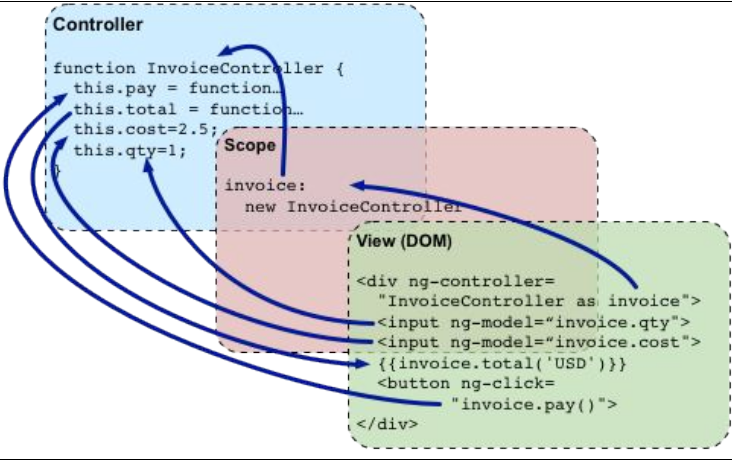
\includegraphics[width=15cm]{imagens/diagrama-angularjs.png}
	\label{imgAngularJS}
	Fonte: \cite{Angular2014}
\end{figure}
\FloatBarrier

\section{Ambiente Virtual de Aprendizagem}

\ac{AVA} � um local virtual que possui um conjunto de elementos tecnol�gicos, onde s�o disponibilizadas ferramentas que permitem o acesso a um ou mais cursos ou disciplinas de uma institui��o de ensino. De modo geral, um AVA refere-se ao uso de recurso digitais de comunica��o, principalmente, atrav�s de softwares educacionais via internet que re�nem diversas ferramentas de intera��o \cite{Oliveira2004, Valentini2005}.

O objetivo de um ambiente virtual de aprendizagem � de facilitar o acesso de alunos ao ensino, pr�ticas de exerc�cios e livros online para consulta. Na Universidade de Caxias do Sul o \ac{AVA} j� � utilizado desde meados de 2005, onde � poss�vel acessar os materiais disponibilizados pelos professores em suas respectivas disciplinas, podendo tamb�m acompanhar o cronograma, entre outras funcionalidades \cite{Oliveira2004, Valentini2005}.

O portal de algoritmos � um ambiente virtual de aprendizagem utilizado pelos alunos da \ac{UCS} nas disciplinas do \ac{CCET}. O portal tem por objetivo auxiliar no ensino da l�gica de programa��o atrav�s da linguagem do portugu�s estruturado \cite{Dorneles2004}.

Vimos at� aqui todos os conceitos necess�rios para o desenvolvimento do trabalho, no cap�tulo a seguir veremos a reengenharia do portal de algoritmos atual, onde � descrita a modelagem e seus problemas de usabilidade e de tecnologia.

\chapter{Avalia��o do Software do Portal de Algoritmos da UCS}\label{cpReengenhariaSoftware}

Nesse cap�tulo � descrita a situa��o atual do sistema, sua modelagem e arquitetura.

\section{Diagrama de Classe de Dom�nio}

O diagrama de classe de dom�nio � a representa��o visual de classes conceituais, ou objetos do mundo real. Tamb�m � chamado de modelo conceitual, que significa uma representa��o de classes conceitos do mundo real, n�o de objetos de \textit{software} \cite{Larman2007}.

Durante a tradu��o do c�digo fonte dos modelos de classes do \textit{Django}, foi constatada nenhuma padroniza��o em nomes de v�riaveis e classes. Abaixo algumas considera��es:

\begin{itemize}
	\item Os campos n�o possuem nomes padronizados utilizando \textit{CamelCase};
	\item Nomes de campos escritos em ingl�s e em portugu�s;
	\item Nomes de classes escritos em ingl�s e em portugu�s;
	\item Nomes de classes n�o s�o intuitivos quanto ao seu objetivo;
\end{itemize}

\textit{CamelCase} � a denomina��o em ingl�s para a pr�tica de escrever palavras compostas, onde cada palavra � iniciada com min�scula ou mai�scula e unidas sem espa�o. Exemplo:

\begin{itemize}
	\item lowerCamelCase;
	\item UpperCamelCase;
\end{itemize}

\newpage

A Figura \ref{imgDominio} representa as classes do portal que � utilizado atualmente.

\FloatBarrier
\begin{figure}[!htb]
	\centering
	\caption{Diagrama de Dom�nio do Portal de Algoritmos Atual}
	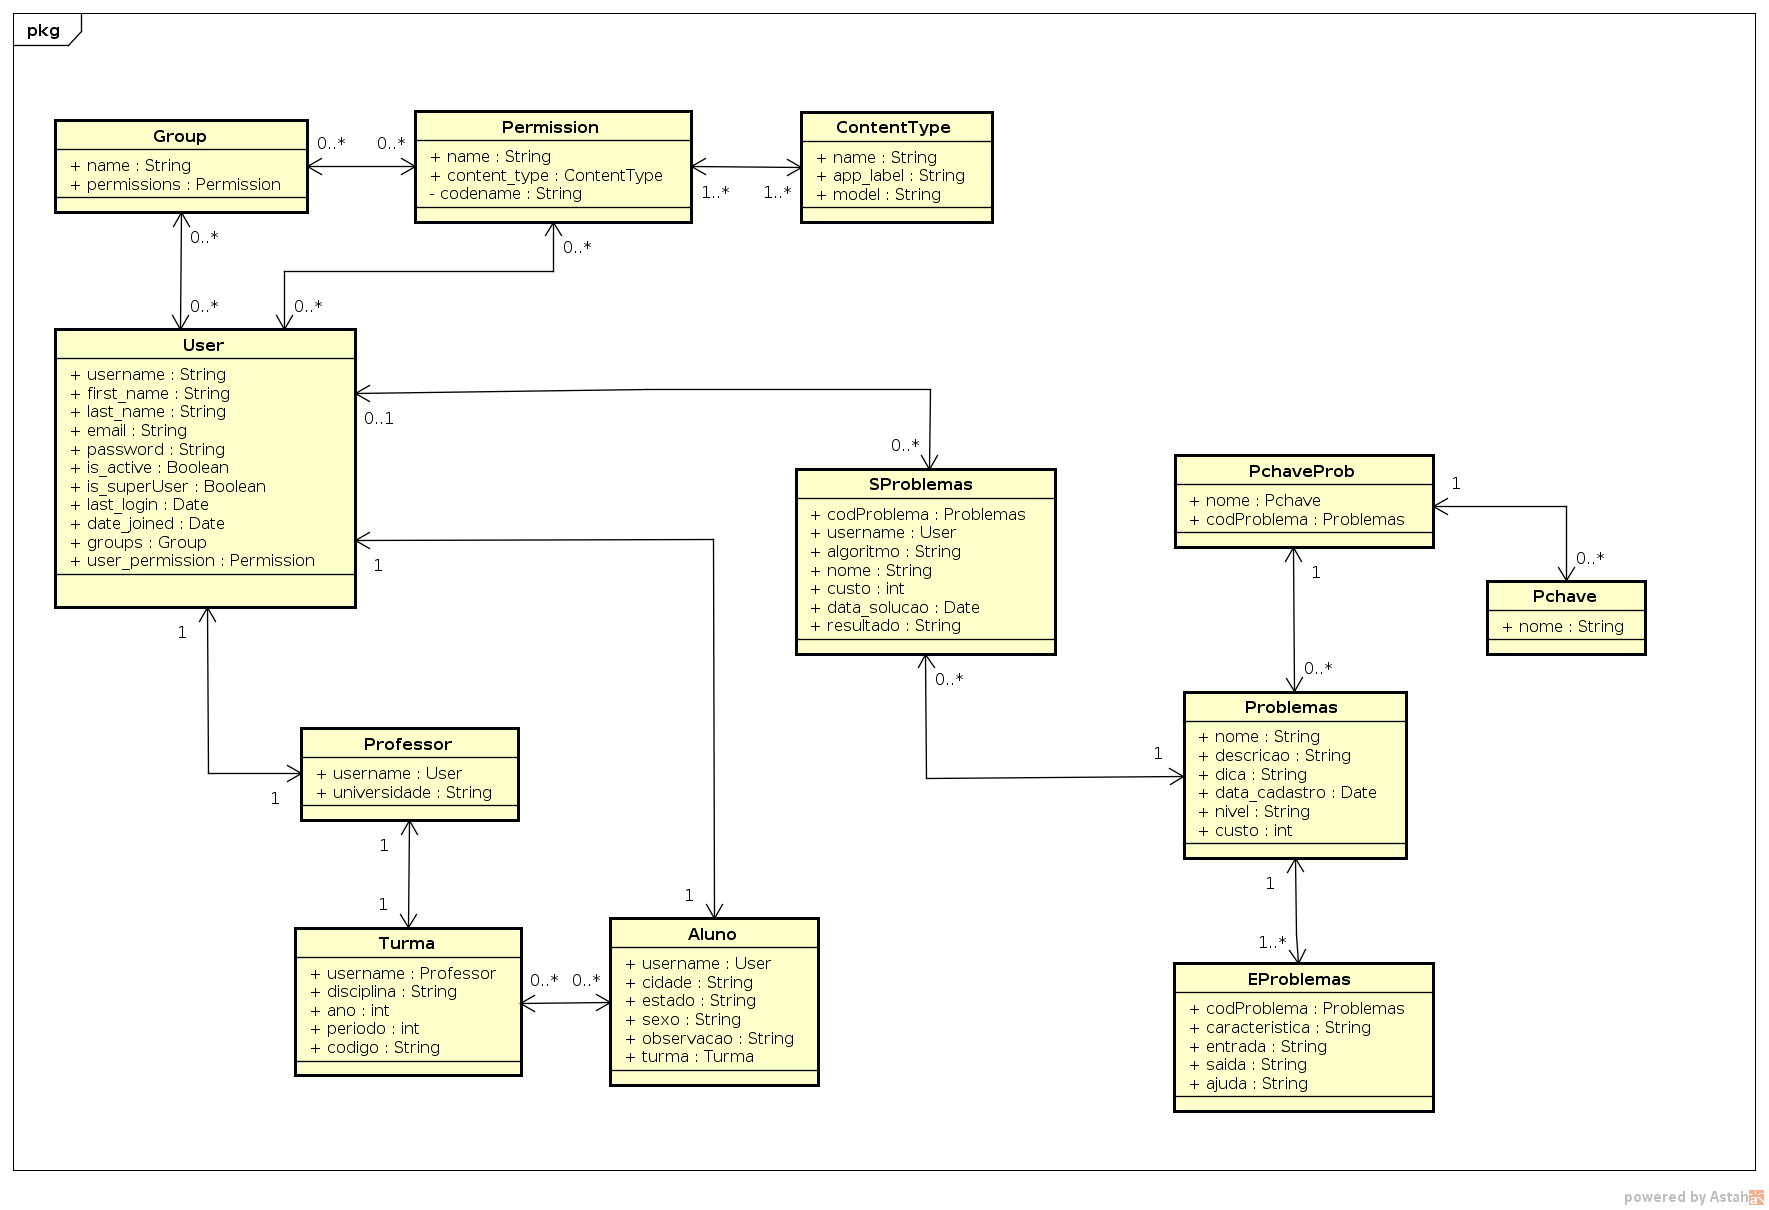
\includegraphics[width=15cm]{UML/portal-atual.png}
	\label{imgDominio}
	Fonte: (AUTOR, 2015)
\end{figure}
\FloatBarrier

A Tabela \ref{tbDescricaoTabelaPortalAntigo} mostra as tabelas do banco de dados e suas descri��es referente ao portal de algoritmos, visa-se manter todas as funcionalidades atuais ap�s a evolu��o do mesmo, e adicionar algumas novas.

\FloatBarrier
\begin{table}[!htb]
	\centering
	\caption{Tabelas do Banco de Dados do Portal de Algoritmos Atual}
	\label{tbDescricaoTabelaPortalAntigo}
	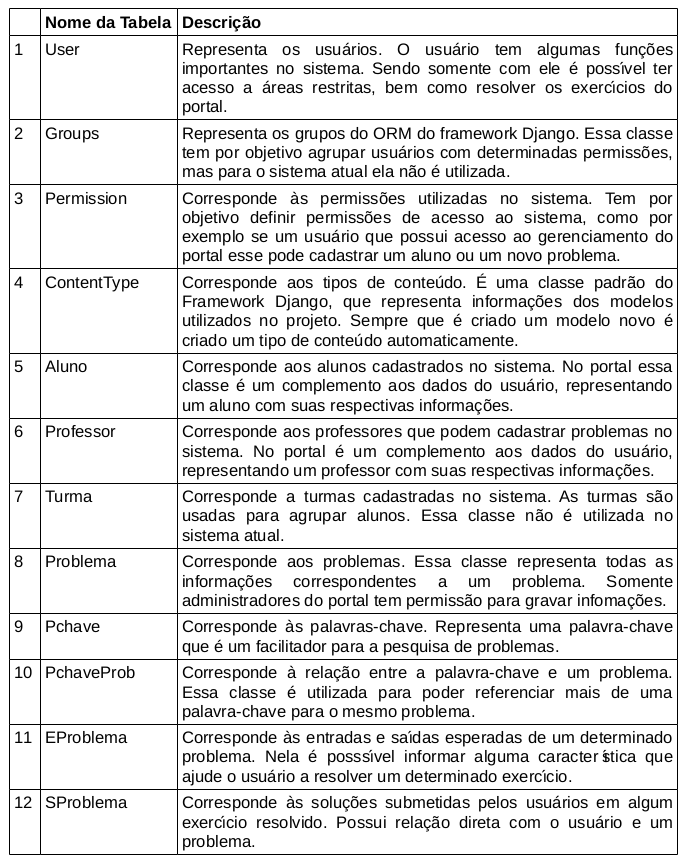
\includegraphics[width=15cm]{UML/classes-de-dominios/1.png}
	Fonte: (AUTOR, 2015)
\end{table}
\FloatBarrier

Nesta se��o foram descritas as classes de dom�nios do portal de algoritmos, a seguir � exibida as interfaces gr�ficas.

\section{Interfaces Gr�ficas}

Nessa se��o s�o descritas as interfaces gr�ficas atuais do software, bem como os problemas encontrados nelas.

\subsection{Cadastro de Aluno}

A Figura \ref{imgCadastroAluno} � a interface de Cadastro de  Aluno, que � realizado pelo pr�prio aluno. As informa��es do aluno ser�o mantidas nas intefaces novas, mantendo assim consist�ncia nas informa��es dos mesmos.

\FloatBarrier
\begin{figure}[!htb]
	\centering
	\caption{Cadastro de Aluno}
	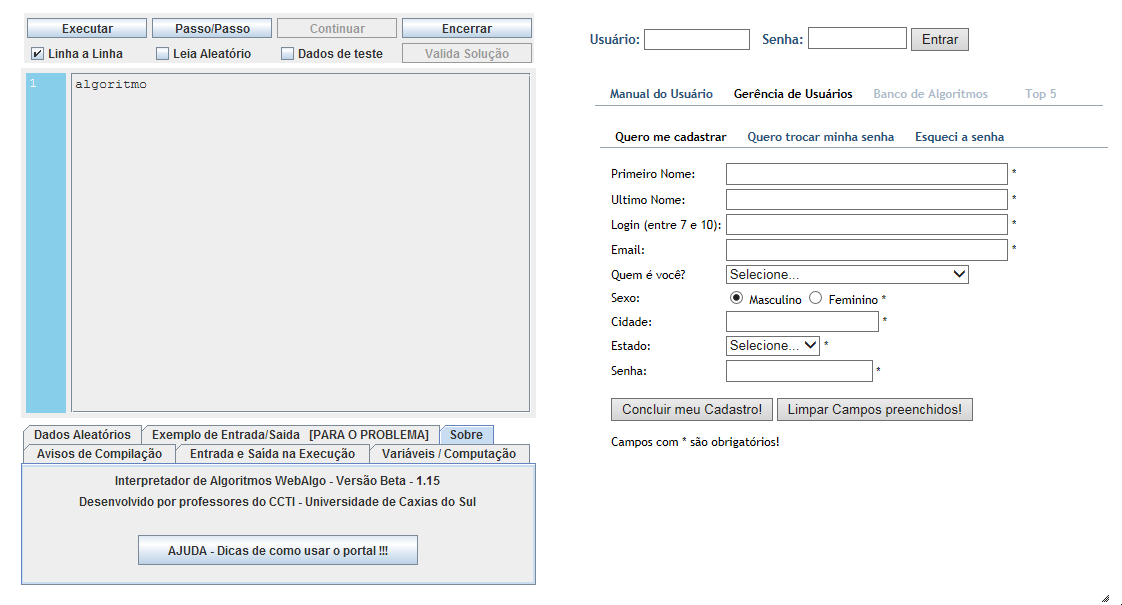
\includegraphics[width=15cm]{imagens/portal-antigo/cadastro-aluno.png}
	\label{imgCadastroAluno}
	Fonte: (AUTOR, 2015)
\end{figure}
\FloatBarrier

Problemas encontrados:

\begin{itemize}
	\item \textit{Java Applet} n�o funciona mais em nenhum navegador de internet atual.
	\item Pouca Usabilidade, uma vez que o cadastro do aluno est� na mesma interface da programa��o de algoritmos.
\end{itemize}

\subsection{Cria��o de Solu��o de Problemas}

A Figura \ref{imgProblemaSelecionado} exibe um aluno j� autenticado no portal e um problema e sua solu��o j� selecionados. Nessa interface gr�fica encontramos as seguintes funcionalidades:

\begin{itemize}
	\item Criar nova solu��o.
	\item Salvar solu��o.
	\item Executar solu��o.
	\item Validar solu��o.
\end{itemize}

\FloatBarrier
\begin{figure}[!htb]
	\centering
	\caption{Cria��o de Solu��o de Problemas}
	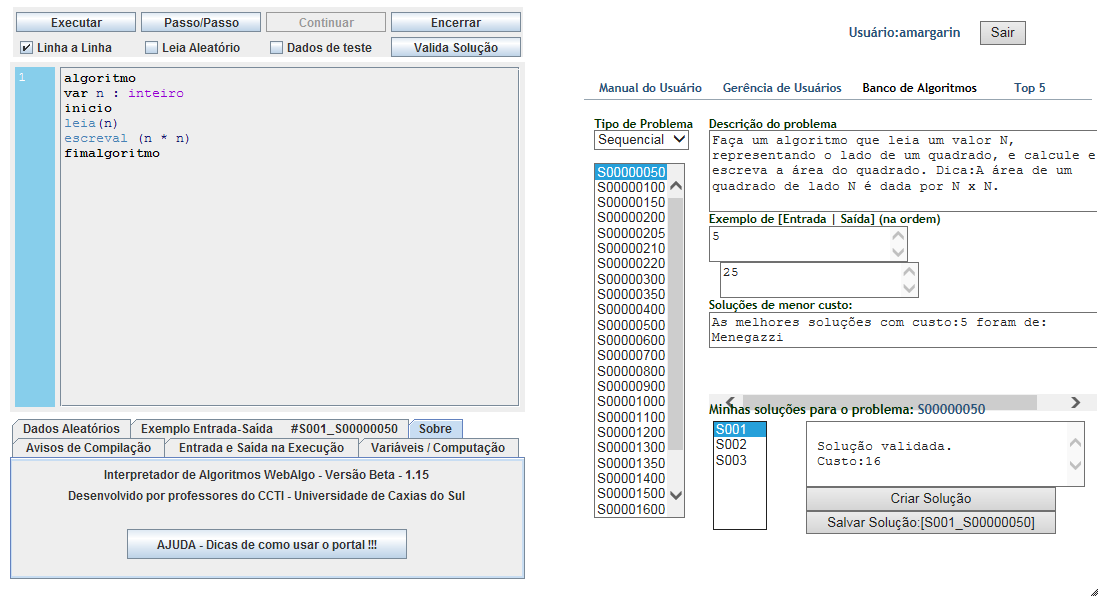
\includegraphics[width=15cm]{imagens/portal-antigo/problema-selecionado.png}
	\label{imgProblemaSelecionado}
	Fonte: (AUTOR, 2015)
\end{figure}

Problemas encontrados:

\begin{itemize}
	\item \textit{Java Applet} n�o funciona mais em nenhum navegador de internet atual.
	\item Pouca Usabilidade, uma vez que para selecionar outro problema s�o necess�rias diversas confirma��es antes de executar a a��o.
\end{itemize}
\FloatBarrier

\newpage

\subsection{Gerenciamento de Alunos}

A Figura \ref{imgAdministracaodeAlunos} � a interface de gerenciamento de alunos. Nessa interface encontramos as seguintes funcionalidades:

\begin{itemize}
	\item Pesquisa de problemas: � poss�vel realizar uma pesquisa livre, entendendo-se por livre qualquer palavra digitada no campos de pesquisa.
	\item Pesquisa de alunos: � poss�vel realizar uma pesquisa livre, entendendo-se por livre qualquer palavra digitada no campos de pesquisa.
	\item Selecionando um problema, automaticamente o sistema faz uma pesquisa dos alunos que j� solucionaram o problema, e selecionando o aluno � realizada uma pesquisa para encontrar as solu��es desse aluno.
	\item Selecionando um aluno, automaticamente o sistema faz uma pesquisa dos problemas que esse aluno j� resolveu, e selecionando o problema � realizada uma pesquisa para encontrar as solu��es desse aluno.
\end{itemize}

\FloatBarrier
\begin{figure}[!htb]
	\centering
	\caption{Ger�ncia de Alunos}
	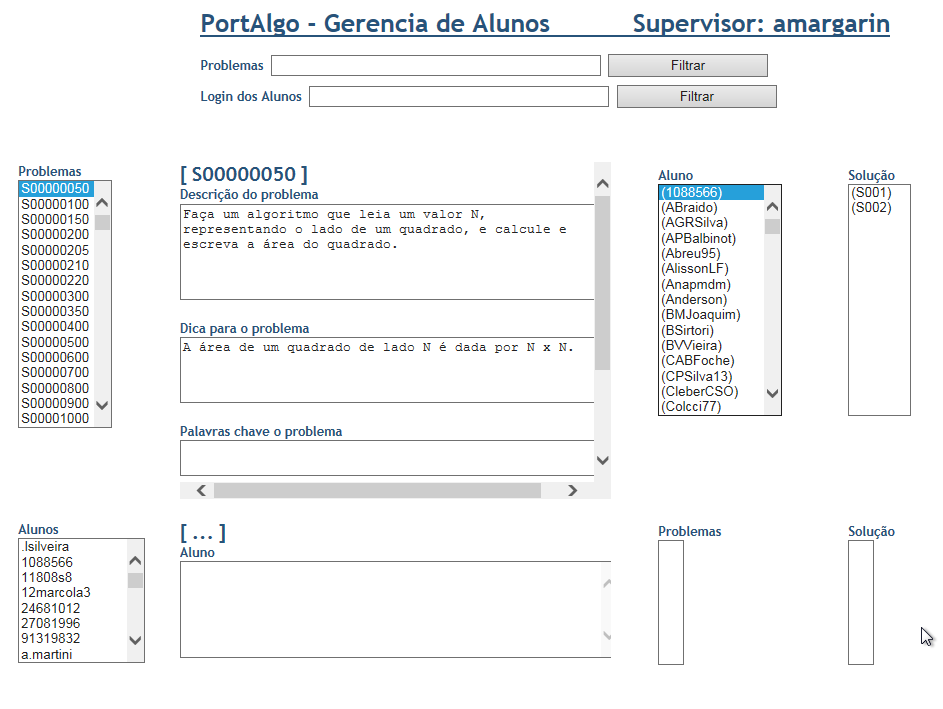
\includegraphics[width=15cm]{imagens/portal-antigo/gerencia-de-alunos.png}
	\label{imgAdministracaodeAlunos}
	Fonte: (AUTOR, 2015)
\end{figure}
\FloatBarrier

Problemas encontrados:

\begin{itemize}
	\item Pouca Usabilidade, uma vez que os campos dispostos na interface de maneira pouco intuitiva ao usu�rio.
\end{itemize}

\subsection{Gerenciamento de Problemas}

A Figura \ref{imgAdministracaodeProblemas} � a interface de gerenciamento de problemas. Nessa interface encontramos as seguintes funcionalidades:

\begin{itemize}
	\item Cadastrar novo problema
	\item Editar um problema:
	\begin{itemize}
		\item Alterar descri��o e dicas
		\item Alterar palavras-chave
		\item Alterar entradas e sa�das
	\end{itemize}
\end{itemize}

\FloatBarrier
\begin{figure}[!htb]
	\centering
	\caption{Ger�ncia de Problemas}
	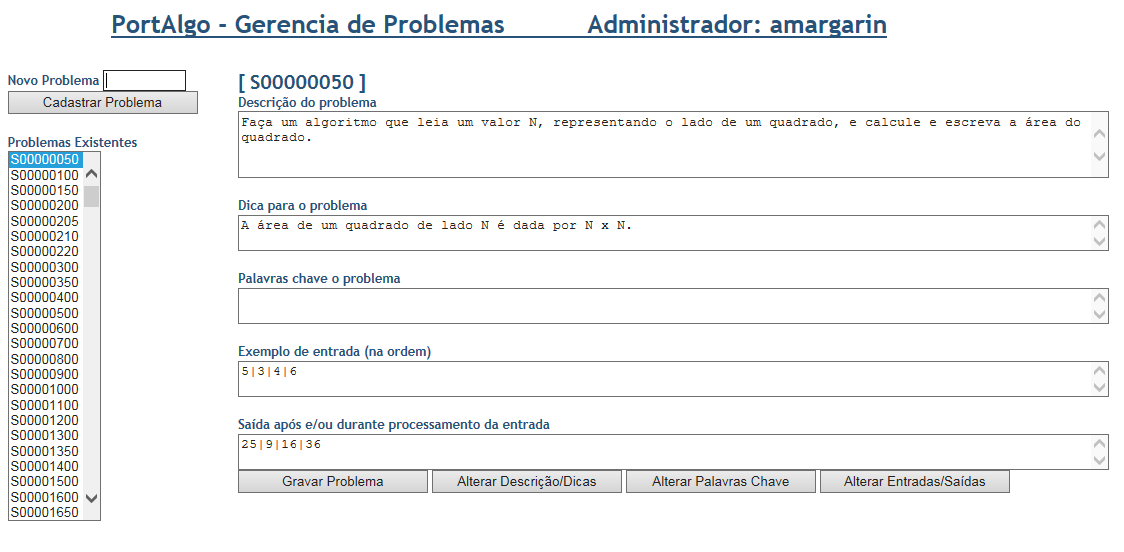
\includegraphics[width=15cm]{imagens/portal-antigo/gerencia-de-problemas.png}
	\label{imgAdministracaodeProblemas}
	Fonte: (AUTOR, 2015)
\end{figure}
\FloatBarrier

Problemas encontrados:

\begin{itemize}
	\item Pouca Usabilidade.
	\begin{itemize}
		\item Campos dispostos na interface de maneira pouco intuitiva ao usu�rio.
		\item N�o possui campo de pesquisa.
		\item A��es descentralizadas que confundem o usu�rio.
	\end{itemize}
\end{itemize}

\newpage

\subsection{Edi��o de Palavra-Chave}

A Figura \ref{imgAdministracaodeProblemasPalavraChave} mostra a mensagem de sucesso ap�s a edi��o de alguma informa��o do problema.

\FloatBarrier
\begin{figure}[!htb]
	\centering
	\caption{Edi��o de palavras-chave}
	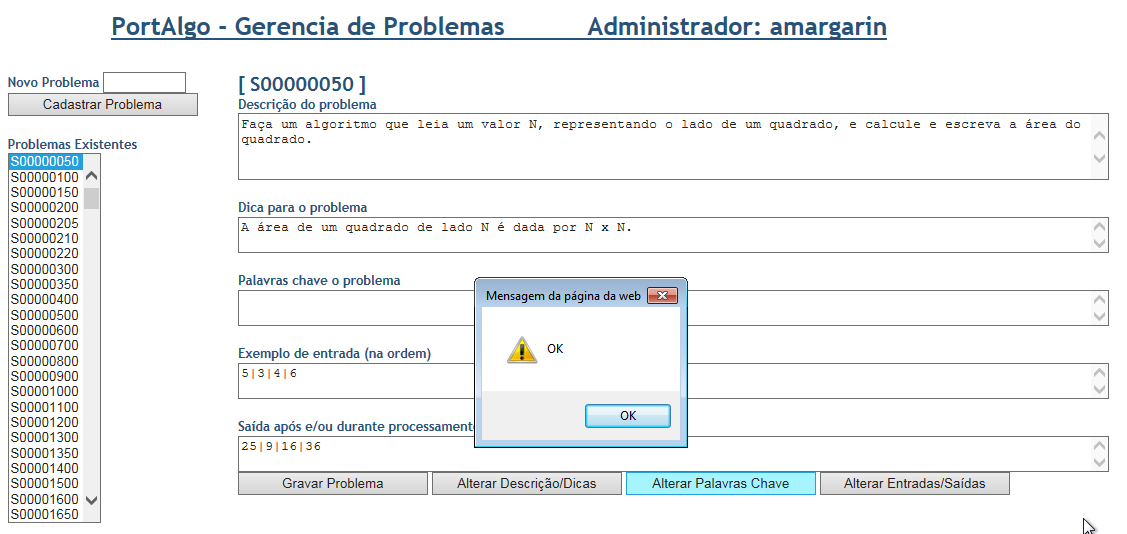
\includegraphics[width=15cm]{imagens/portal-antigo/gerencia-de-problemas-editando-palavras-chaves.png}
	\label{imgAdministracaodeProblemasPalavraChave}
	Fonte: (AUTOR, 2015)
\end{figure}
\FloatBarrier

Problemas encontrados:

\begin{itemize}
	\item Pouca Usabilidade: a mensagem n�o possui uma informa��o clara do que foi editado, ou o que foi realizado.
\end{itemize}

\newpage

\subsection{Solu��o de Problemas}

A Figura \ref{imgAdministracaodeProblemasSolucao} exibe a solu��o de um problema em uma nova janela.

\FloatBarrier
\begin{figure}[!htb]
	\centering
	\caption{Visualizando solu��o de um aluno}
	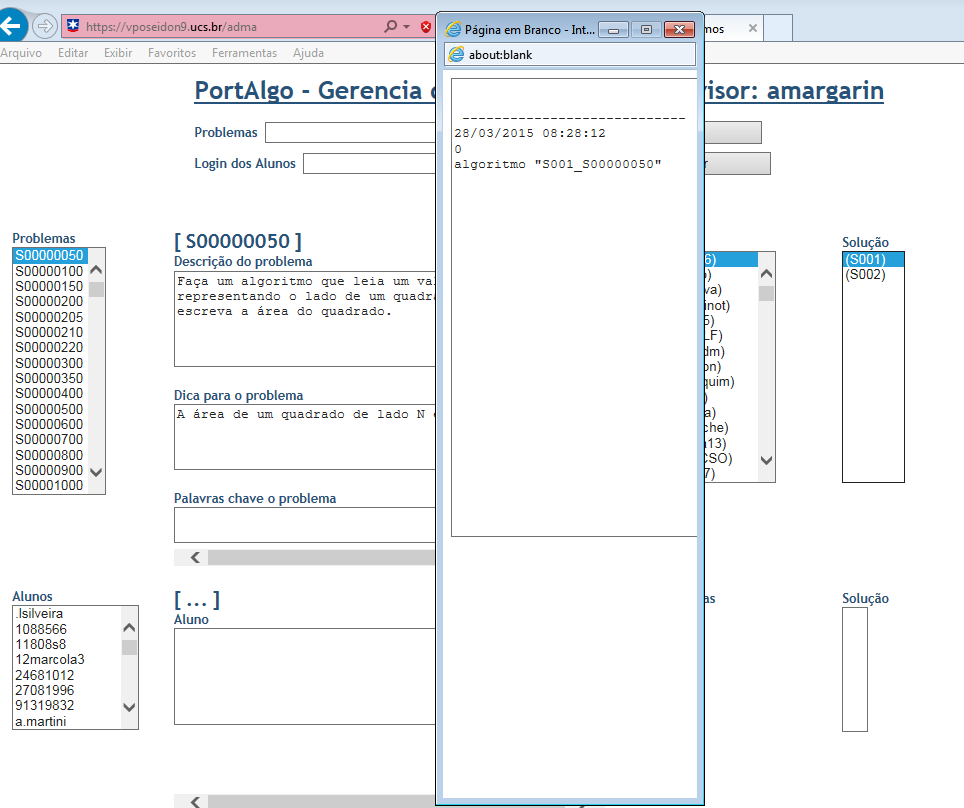
\includegraphics[width=15cm]{imagens/portal-antigo/administracao-de-problemas-visualizando-solucao-partindo-do-problema.png}
	\label{imgAdministracaodeProblemasSolucao}
	Fonte: (AUTOR, 2015)
\end{figure}
\FloatBarrier

Problemas encontrados:

\begin{itemize}
	\item Pouca Usabilidade.
	\begin{itemize}
		\item A nova janela que � aberta � muito pequena e sem a possibilidade de aumentar.
		\item N�o � poss�vel editar.
	\end{itemize}
\end{itemize}


Os problemas encontrados no \textit{software} atual prejudicam a usabilidade do mesmo. Atualmente ele est� limitado a apenas um navegador de internet, no caso o \textit{Internet Explorer}.

Para solucionar e deix�-lo mais us�vel, fazendo com que mais alunos sejam beneficiados pelo portal, bem como facilitando o uso por parte dos professores,  no pr�ximo cap�tulo ser� descrita toda a modelagem, novas interfaces e novas funcionalidades, utilizando-se de tecnologias mais atuais.


\chapter{Proposta de Solu��o}\label{cpProposta}

O presente trabalho tem por objetivo realizar a evolu��o do gerenciamento do portal de algoritmos. Para tanto, foi realizada a engenharia reversa do \textit{software} atual, atrav�s da an�lise do c�digo fonte, suas funcionalidades, sua arquitetura e seu banco de dados.

Para descrever a evolu��o de \textit{software}, nas se��es seguintes ser�o apresentados conceitos e artefatos da engenharia de \textit{software}. O \textit{software} ser� modelado utilizando-se de artefatos da metodologia ICONIX ser� modelado o \textit{software}.

A solu��o proposta ser� desenvolvida na linguagem de programa��o Java, a fim de unificar as tecnologias do gerenciamento do portal de algoritmos com seu analisador algor�tmico.

O \textit{software} ser� constru�do com uma arquitetura orientada a servi�os, cujo objetivo � que ele seja disponibilizado em interfaces, ou seja, seja acess�vel atrav�s de \ac{REST}.

Na evolu��o do \textit{software} ser�o mantidas as funcionalidades atuais e adicionadas novas funcionalidades.

Funcionalidades que ser�o mantidas s�o:

\begin{itemize}
	\item Manter Usu�rios.
	\item Manter Permiss�es.
	\item Manter Tipos de Problemas.
	\item Manter Problemas.
	\item Manter Entradas e Sa�das
	\item Manter Palavras-chave
	\item Manter Solu��es de Problemas
\end{itemize}

Novas funcionalidades:

\begin{itemize}
	\item Manter Grupos de Administradores.
	\item Manter Alunos e Professores.
	\item Manter Grupos de Alunos.
	\item Manter Institui��es.
	\item Manter Pa�ses, Estados e Cidades.
\end{itemize}

\section{Diagrama de Classe de Dom�nio}\label{scDiagramaClasse}

A Figura \ref{imgDiagramaNovo} representa o diagrama de classe de dom�nio proposto para a evolu��o do portal de algoritmos. Nesse novo diagrama foram melhoradas as descri��es dos campos, descrevendo-os em ingl�s.

\FloatBarrier
\begin{figure}[!htb]
	\centering
	\caption{Diagrama de Dom�nio do Portal de Algoritmos Novo}
	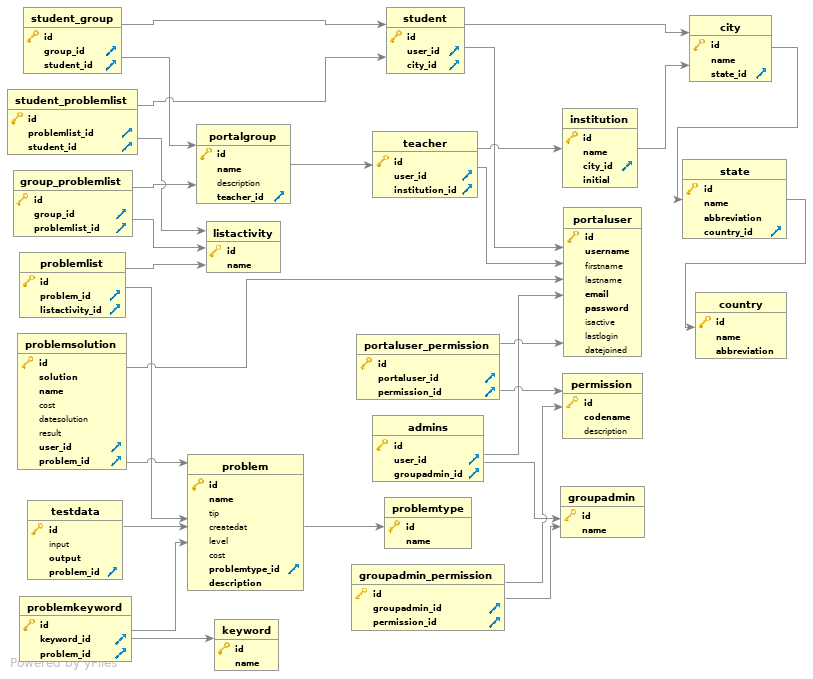
\includegraphics[width=15cm]{UML/diagrama-portal-novo.png}
	\label{imgDiagramaNovo}
	Fonte: (AUTOR, 2018)
\end{figure}
\FloatBarrier

A Tabela \ref{tbDescricaoTabelaPortalNovo} mostra as tabelas do banco de dados e suas descri��es referente ao portal de algoritmos.

\FloatBarrier
\begin{table}[!htb]
	\centering
	\caption{Tabelas do Banco de Dados do Portal de Algoritmos Novo}
	\label{tbDescricaoTabelaPortalNovo}
	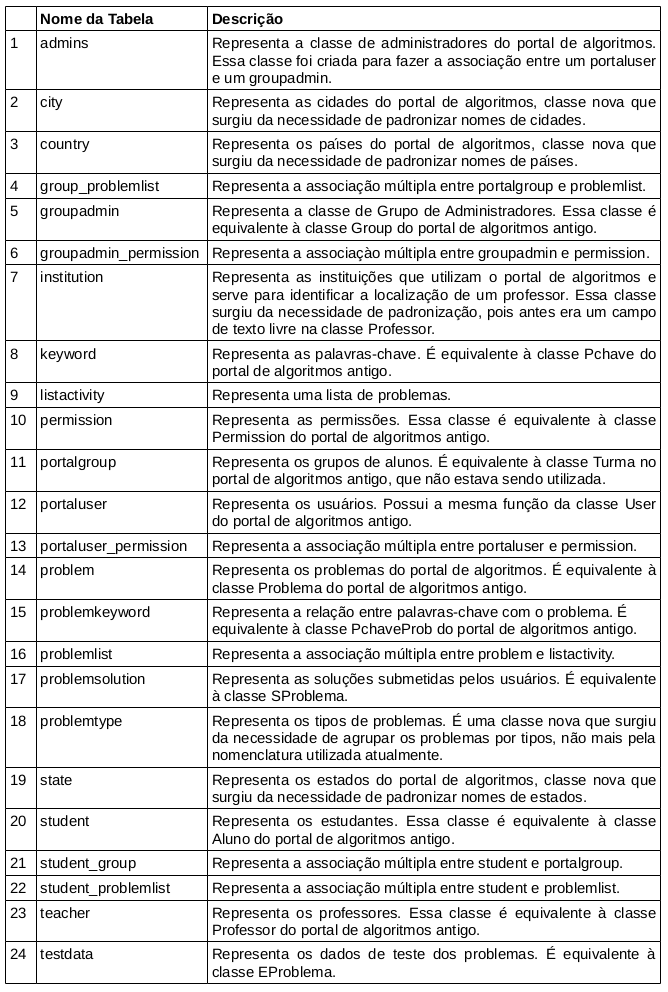
\includegraphics[width=15cm]{UML/classes-de-dominios/2.png}
	Fonte: (AUTOR, 2018)
\end{table}
\FloatBarrier

Ao realizar a modelagem do diagrama de classes de dom�nios do novo portal de algoritmos, foram padronizados nomes das tabelas e colunas, de uma forma a ser mais descritivos. Na se��o seguinte s�o descritos os requisitos funcionais e n�o-funcionais do projeto.

\section{Requisitos de projeto}

Antes do desenvolvimento do \textit{software} � preciso realizar o levantamento de requisitos funcionais e n�o-funcionais. Esses requisitos descrevem o que o sistema deve fazer e suas restri��es.

\subsection{Requisitos Funcionais}

A Tabela \ref{tbRequisitoFuncionais} mostra os requisitos funcionais do portal de algoritmos. Nesta Tabela entende-se quando se refere em ``manter", listar, cadastrar, editar e deletar um objeto.

\FloatBarrier
\begin{table}[!htb]
	\centering
	\caption{Requisitos funcionais}
	\label{tbRequisitoFuncionais}
	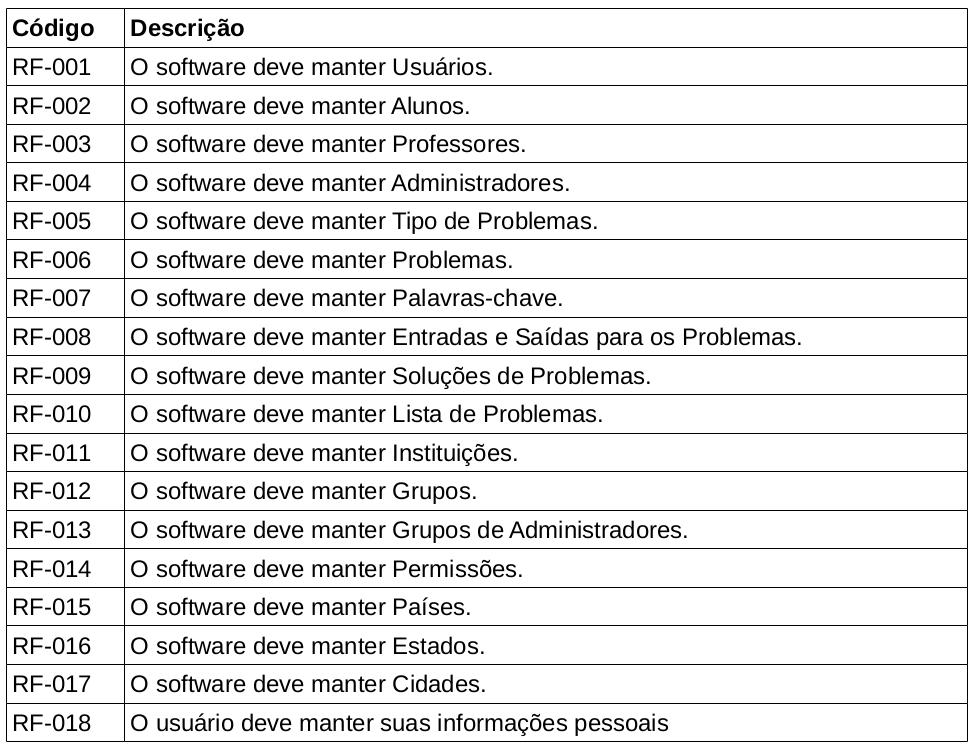
\includegraphics[width=15cm]{UML/requisitos/1.png}
	Fonte: (AUTOR, 2018)
\end{table}
\FloatBarrier

\newpage

\subsection{Requisitos N�o-Funcionais}

A Tabela \ref{tbRequisitosNaoFuncionais} s�o os requisitos n�o-funcionais do portal de algoritmos.

\FloatBarrier
\begin{table}[!htb]
	\centering
	\caption{Requisitos n�o-funcionais}
	\label{tbRequisitosNaoFuncionais}
	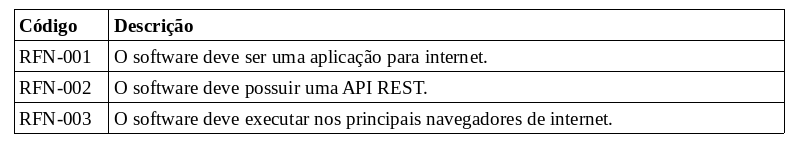
\includegraphics[width=15cm]{UML/requisitos/2.png}
	Fonte: (AUTOR, 2018)
\end{table}
\FloatBarrier

Cada requisito funcional elicitado pode se tornar um caso de uso. Esses casos de uso ser�o descritos na se��o seguinte.

\section{Casos de Uso}

Ap�s o levantamento e descri��o dos requisitos do \textit{software}, pode ser criado o diagrama macro de intera��o entre o usu�rio e os casos de uso do sistema, ressaltando que um \textit{software} dessa natureza deve ter um ambiente de execu��o com acesso a \textit{internet}.

Na Figura \ref{imgCasoUsoAdministrador} est�o representados os casos de uso em que o ator ``Administrador" \ est� envolvido para o gerenciamento do portal.

\FloatBarrier
\begin{figure}[!htb]
	\centering
	\caption{Casos de Uso que envolvem o ator Administrador}
	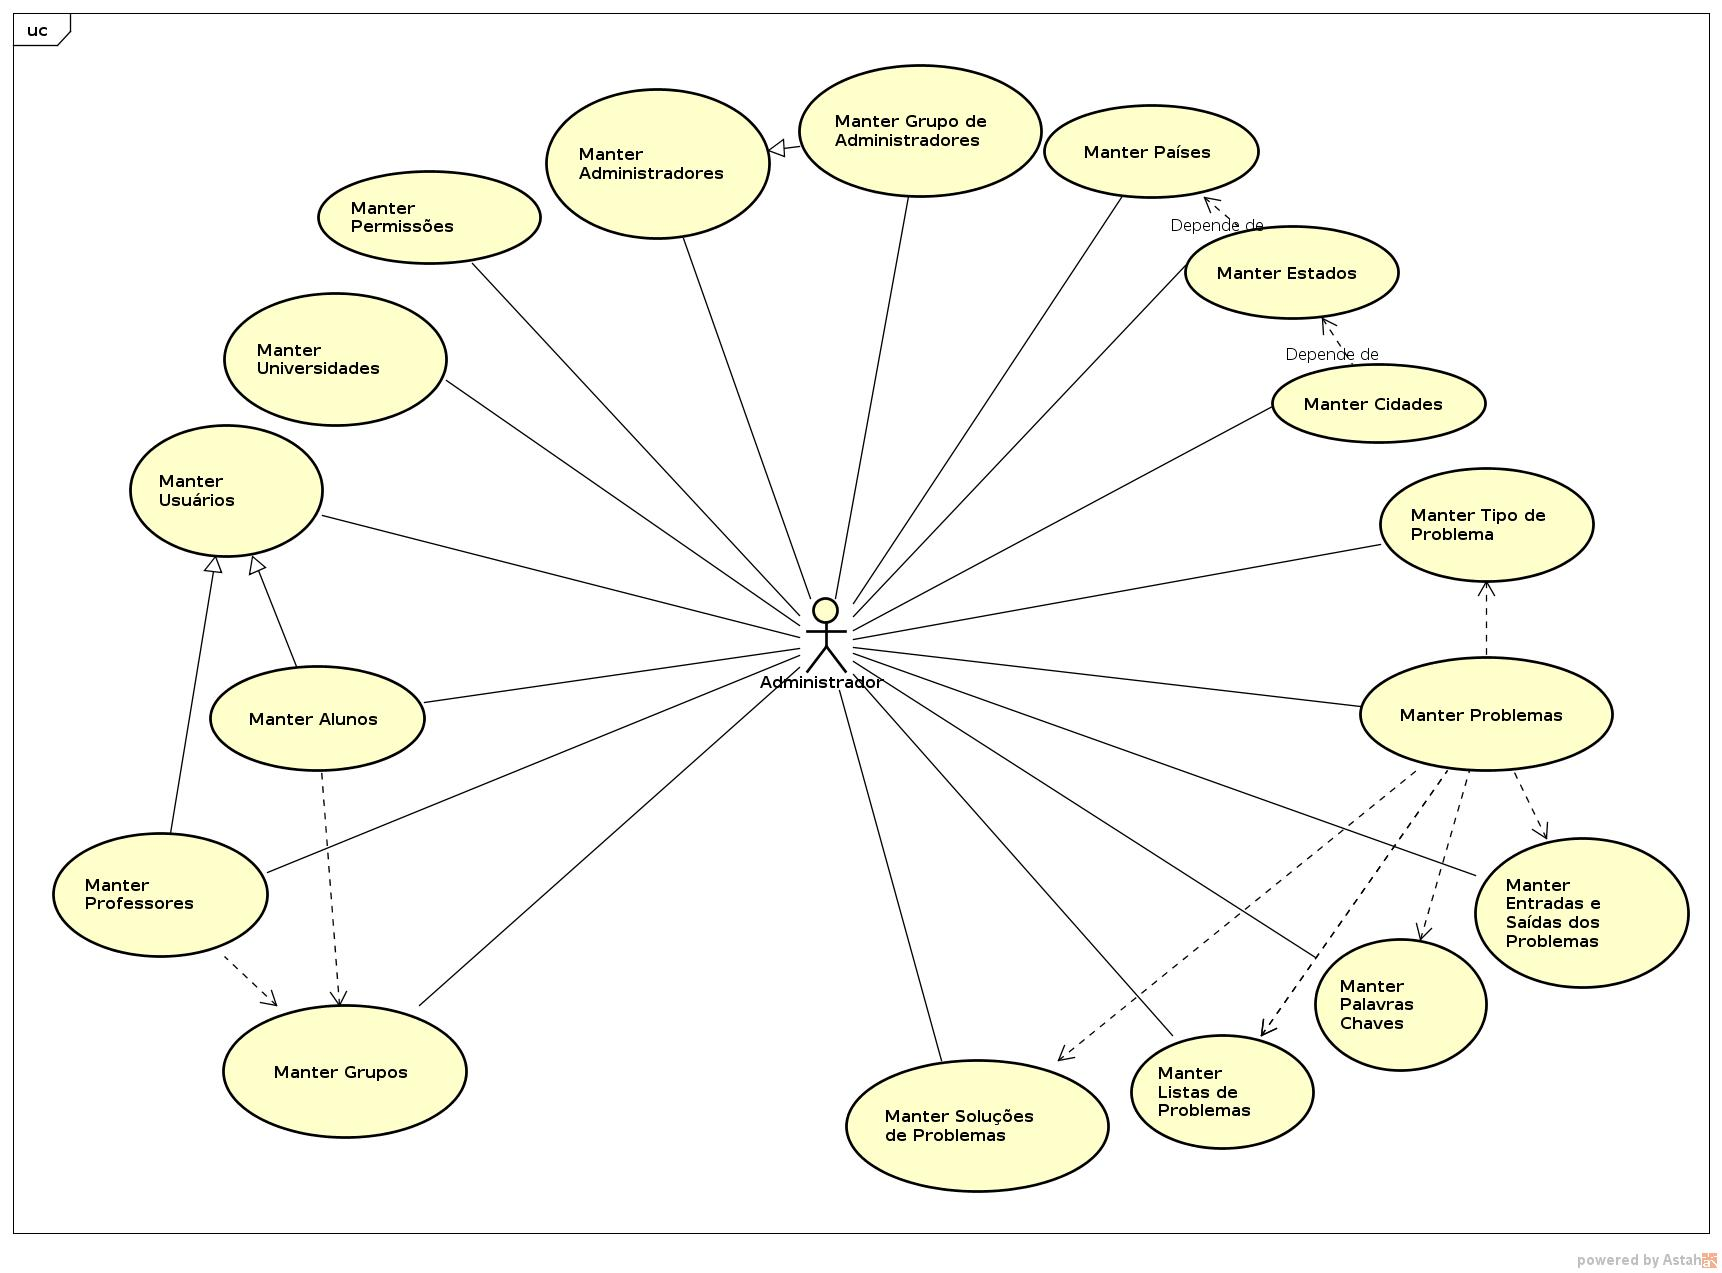
\includegraphics[width=15cm]{UML/casos-de-uso-administrador.jpg}
	\label{imgCasoUsoAdministrador}
	Fonte: (AUTOR, 2018)
\end{figure}
\FloatBarrier

Na Figura \ref{imgCasoUsoProfessor} est�o representados os casos de uso em que o ator ``Professor" \ est� envolvido para o gerenciamento do portal.

\FloatBarrier
\begin{figure}[!htb]
	\centering
	\caption{Casos de Uso que envolvem o ator Professor}
	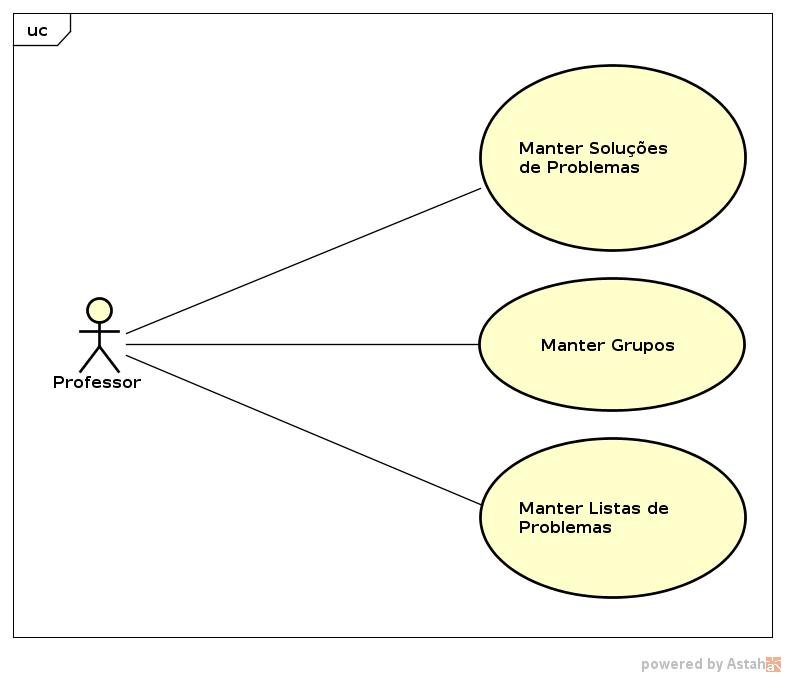
\includegraphics[width=8cm]{UML/casos-de-uso-professor.jpg}
	\label{imgCasoUsoProfessor}
	\\
	Fonte: (AUTOR, 2018)
\end{figure}
\FloatBarrier

\newpage

Na Figura \ref{imgCasoUsoAluno} est�o representados os casos de uso em que o ator ``Aluno" \ est� envolvido para o gerenciamento do portal.

\FloatBarrier
\begin{figure}[!htb]
	\centering
	\caption{Casos de Uso que envolvem o ator Aluno}
	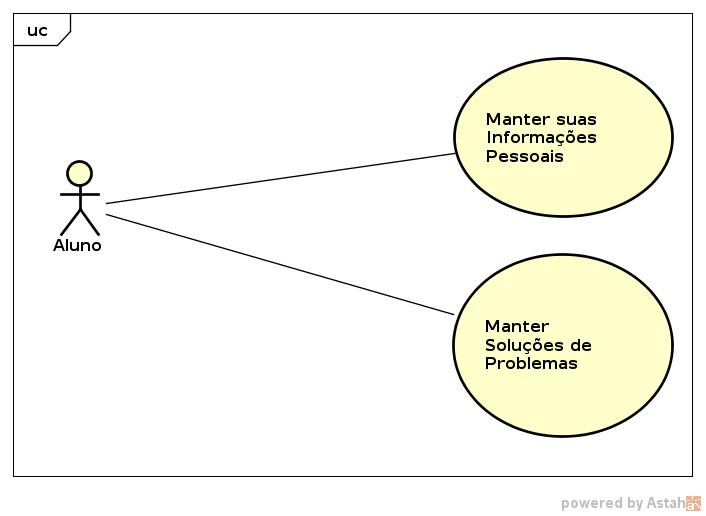
\includegraphics[width=8cm]{UML/casos-de-uso-aluno.jpg}
	\label{imgCasoUsoAluno}
	\\
	Fonte: (AUTOR, 2018)
\end{figure}
\FloatBarrier

A seguir s�o apresentados detalhadamente cada um dos caso de uso apresentados nas Figuras \ref{imgCasoUsoAdministrador}, \ref{imgCasoUsoProfessor} e \ref{imgCasoUsoAluno}. Ser�o apresentados os fluxos de execu��o principais e alternativos de cada caso de uso.

\newpage

\subsection{Descri��o dos Casos de Uso}

Nesta se��o s�o descritos os casos de uso levantados a partir dos requisitos funcionais.

\subsubsection{Manter Usu�rios}

A Tabela \ref{imgManterUsuarios} descreve o caso de uso de manter o cadastro, edi��o e remo��o das informa��es dos usu�rios. Esse caso de uso possui um �nico ator, o "Administrador" e a pr�-condi��o � ser um administrador do sistema.

\FloatBarrier
\begin{table}[!htb]
	\centering
	\caption{Caso de Uso Manter Usu�rios}
	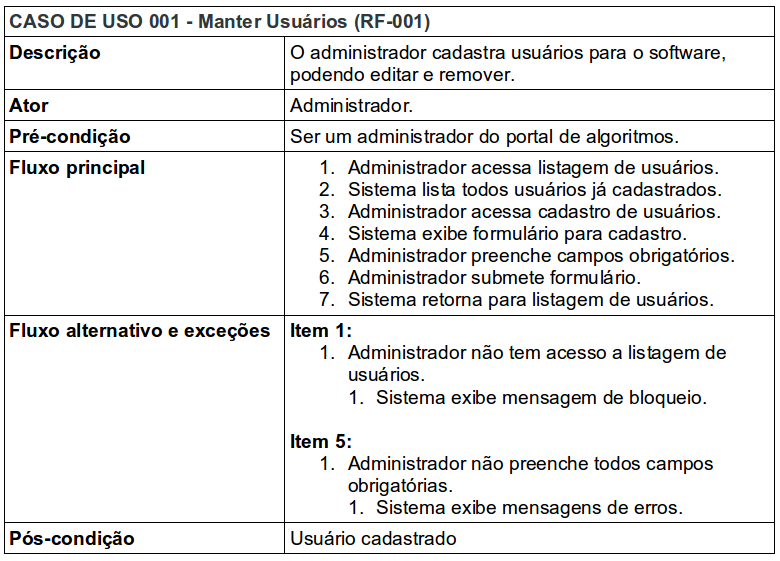
\includegraphics[width=15cm]{UML/casos-de-uso/1.png}
	\label{imgManterUsuarios}
	Fonte: (AUTOR, 2018)
\end{table}
\FloatBarrier

\newpage

\subsubsection{Manter Alunos}

A Tabela \ref{imgManterAlunos} descreve o caso de uso de manter o cadastro, edi��o e remo��o das informa��es dos alunos. Esse caso de uso possui um �nico ator, o ``Administrador" e possui duas pr�-condi��es, ser administrador do sistema e o aluno precisa estar associado a um usu�rio.

\FloatBarrier
\begin{table}[!htb]
	\centering
	\caption{Caso de Uso Manter Alunos}
	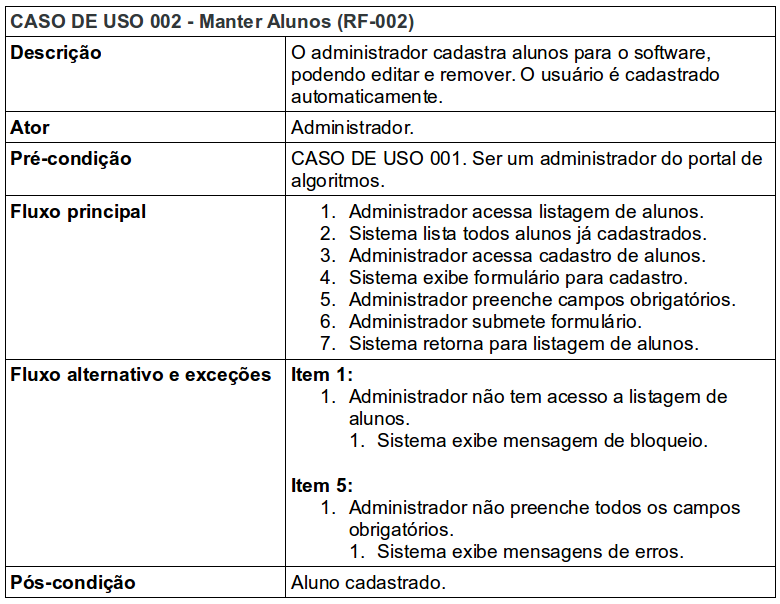
\includegraphics[width=15cm]{UML/casos-de-uso/2.png}
	\label{imgManterAlunos}
	Fonte: (AUTOR, 2018)
\end{table}
\FloatBarrier

\newpage

\subsubsection{Manter Professores}

A Tabela \ref{imgManterProfessores} descreve o caso de uso de manter o cadastro, edi��o e remo��o das informa��es dos professores. Esse caso de uso possui um �nico ator, o ``Administrador" e possui duas pr�-condi��es, ser administrador do sistema e o professor precisa estar associado a um usu�rio.

\FloatBarrier
\begin{table}[!htb]
	\centering
	\caption{Caso de Uso Manter Professores}
	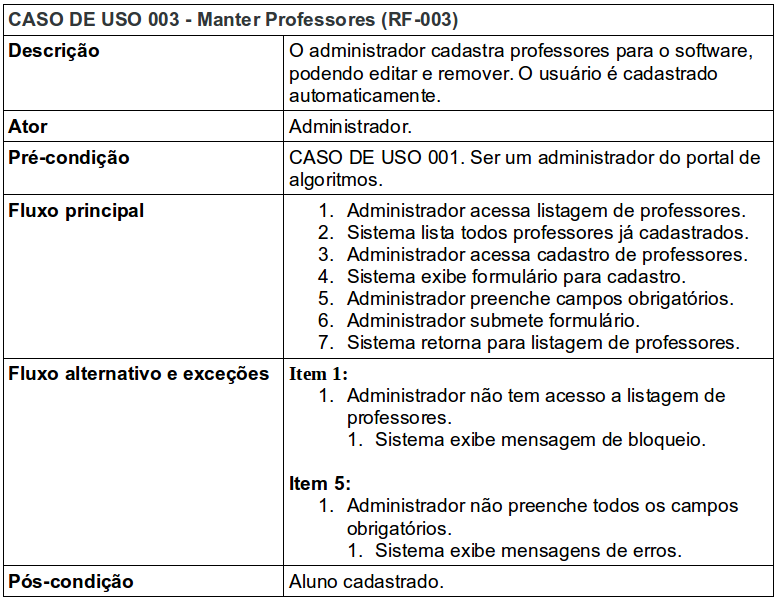
\includegraphics[width=15cm]{UML/casos-de-uso/3.png}
	\label{imgManterProfessores}
	Fonte: (AUTOR, 2018)
\end{table}
\FloatBarrier

\newpage

\subsubsection{Manter Administradores}

A Tabela \ref{imgManterAdministradores} descreve o caso de uso de manter o cadastro, edi��o e remo��o das informa��es dos administradores do sistema. Esse caso de uso possui um �nico ator, o ``Administrador", possui duas pr�-condi��es, ser um administrador do sistema e possuir um usu�rio para adicionar como administrador do sistema.

\FloatBarrier
\begin{table}[!htb]
	\centering
	\caption{Caso de Uso Manter Administradores}
	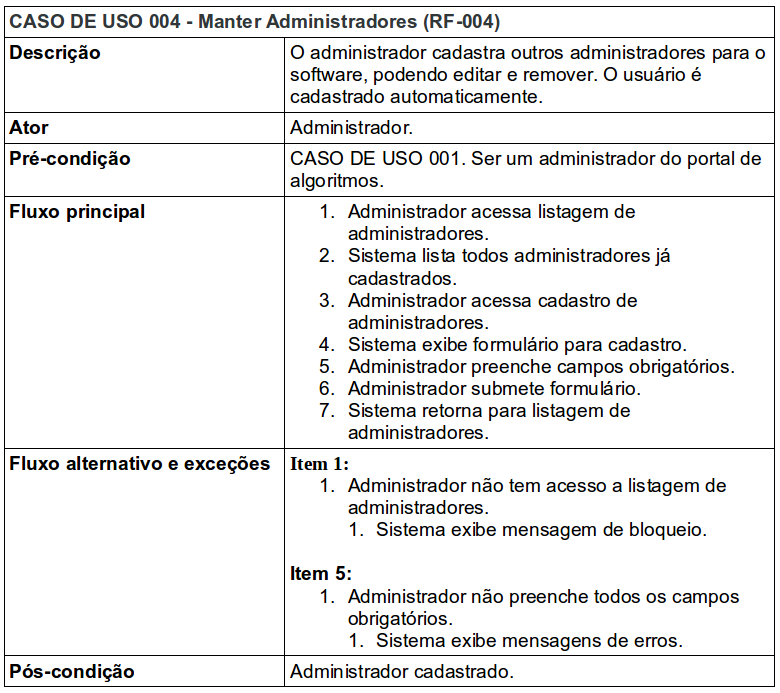
\includegraphics[width=15cm]{UML/casos-de-uso/4.png}
	\label{imgManterAdministradores}
	Fonte: (AUTOR, 2018)
\end{table}
\FloatBarrier

\newpage

\subsubsection{Manter Tipo de Problema}

A Tabela \ref{imgManterTipoProblemas} descreve o caso de uso de manter o cadastro, edi��o e remo��o das informa��es de um tipo de problema. Um tipo de problema serve para agrupar problemas que possuem rela��o.

\FloatBarrier
\begin{table}[!htb]
	\centering
	\caption{Caso de Uso Manter Tipo de Problema}
	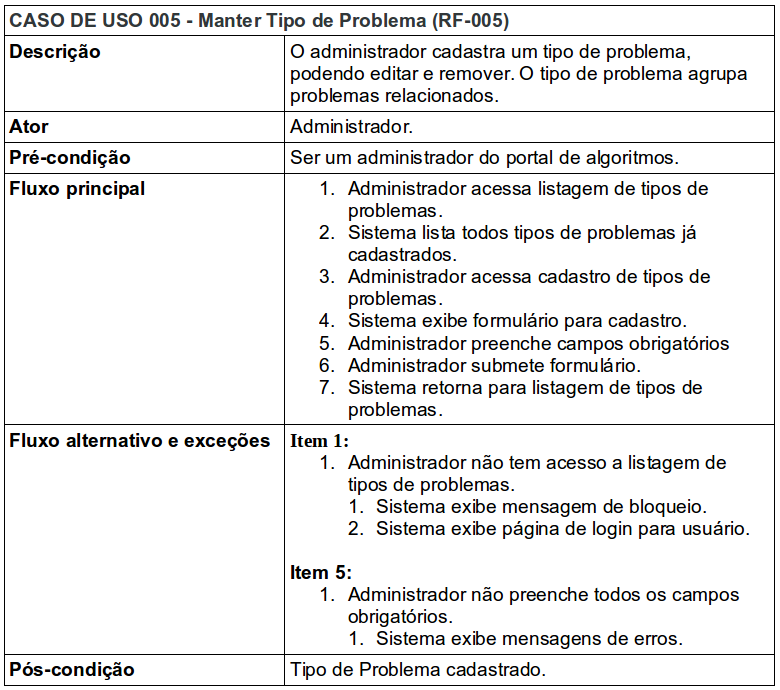
\includegraphics[width=15cm]{UML/casos-de-uso/5.png}
	\label{imgManterTipoProblemas}
	Fonte: (AUTOR, 2018)
\end{table}
\FloatBarrier

\newpage

\subsubsection{Manter Problemas}

A Tabela \ref{imgManterProblemas} descreve o caso de uso de manter o cadastro, edi��o e remo��o das informa��es de problemas.

\FloatBarrier
\begin{table}[!htb]
	\centering
	\caption{Caso de Uso Manter Problemas}
	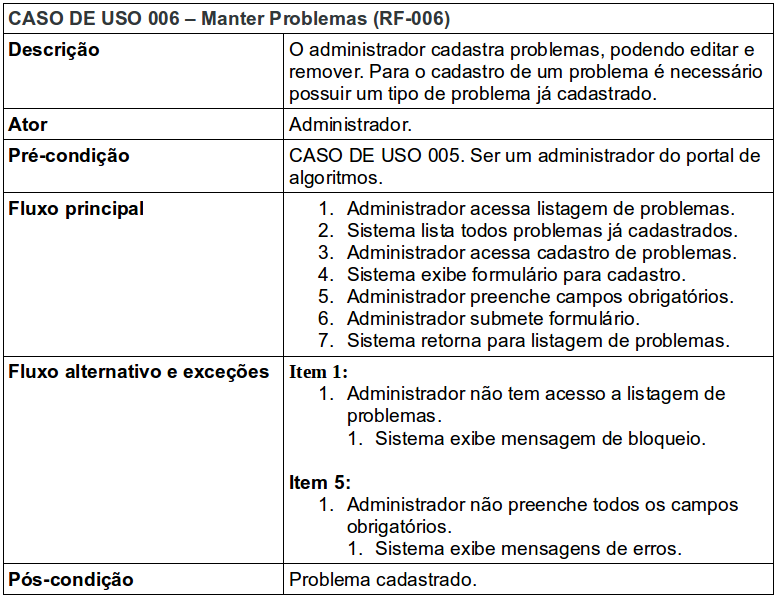
\includegraphics[width=15cm]{UML/casos-de-uso/6.png}
	\label{imgManterProblemas}
	Fonte: (AUTOR, 2018)
\end{table}
\FloatBarrier

\newpage

\subsubsection{Manter Palavras-chave}

A Tabela \ref{imgManterPalavrasChaves} descreve o caso de uso de manter o cadastro, edi��o e remo��o das informa��es das palavras-chave de um ou mais problemas.

\FloatBarrier
\begin{table}[!htb]
	\centering
	\caption{Caso de Uso Manter Palavras-chave}
	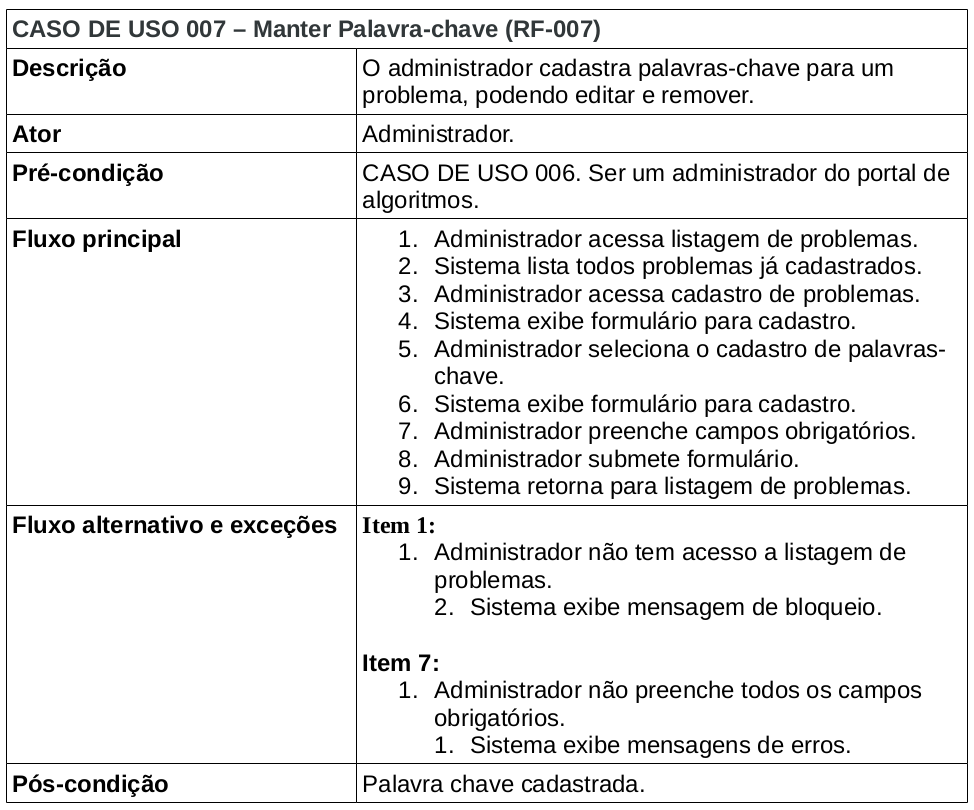
\includegraphics[width=15cm]{UML/casos-de-uso/7.png}
	\label{imgManterPalavrasChaves}
	Fonte: (AUTOR, 2018)
\end{table}
\FloatBarrier

\newpage

\subsubsection{Manter Entradas e Sa�das}

A Tabela \ref{imgManterEntradasSaidas} descreve o caso de uso de manter o cadastro, edi��o e remo��o das informa��es das entradas e sa�das de um determinado problema.

\FloatBarrier
\begin{table}[!htb]
	\centering
	\caption{Caso de Uso Manter Entrada e Sa�das}
	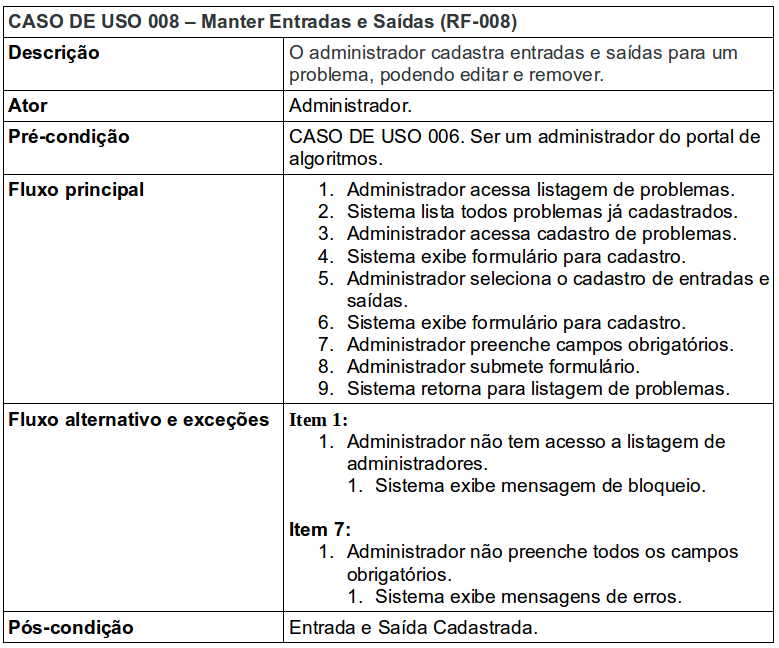
\includegraphics[width=15cm]{UML/casos-de-uso/8.png}
	\label{imgManterEntradasSaidas}
	Fonte: (AUTOR, 2018)
\end{table}
\FloatBarrier

\newpage

\subsubsection{Manter Solu��es de Problemas}

A Tabela \ref{imgManterSolucoesProblemas} descreve o caso de uso de manter o cadastro, edi��o e remo��o das solu��es de um determinado problema. As solu��es podem ser cadastradas por administradores, professores e/ou alunos.

\FloatBarrier
\begin{table}[!htb]
	\centering
	\caption{Caso de Uso Manter Solu��es de Problemas}
	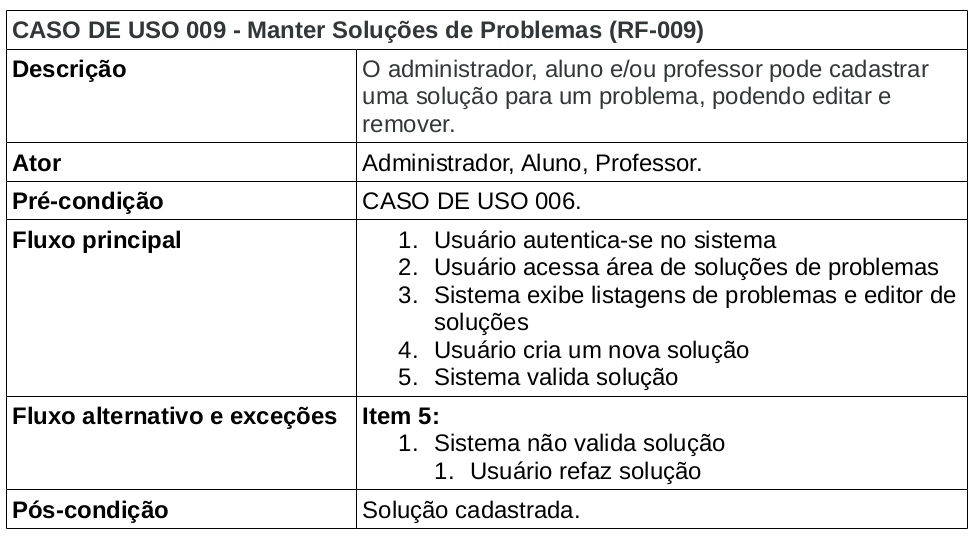
\includegraphics[width=15cm]{UML/casos-de-uso/9.png}
	\label{imgManterSolucoesProblemas}
	Fonte: (AUTOR, 2018)
\end{table}
\FloatBarrier

\newpage

\subsubsection{Manter Listas de Problemas}

A Tabela \ref{imgManterListaProblemas} descreve o caso de uso de manter o cadastro, edi��o e remo��o das listas de problemas. Essas listas agrupam problemas para serem aplicados a um grupo e/ou aluno.

\FloatBarrier
\begin{table}[!htb]
	\centering
	\caption{Caso de Uso Manter Listas de Problemas}
	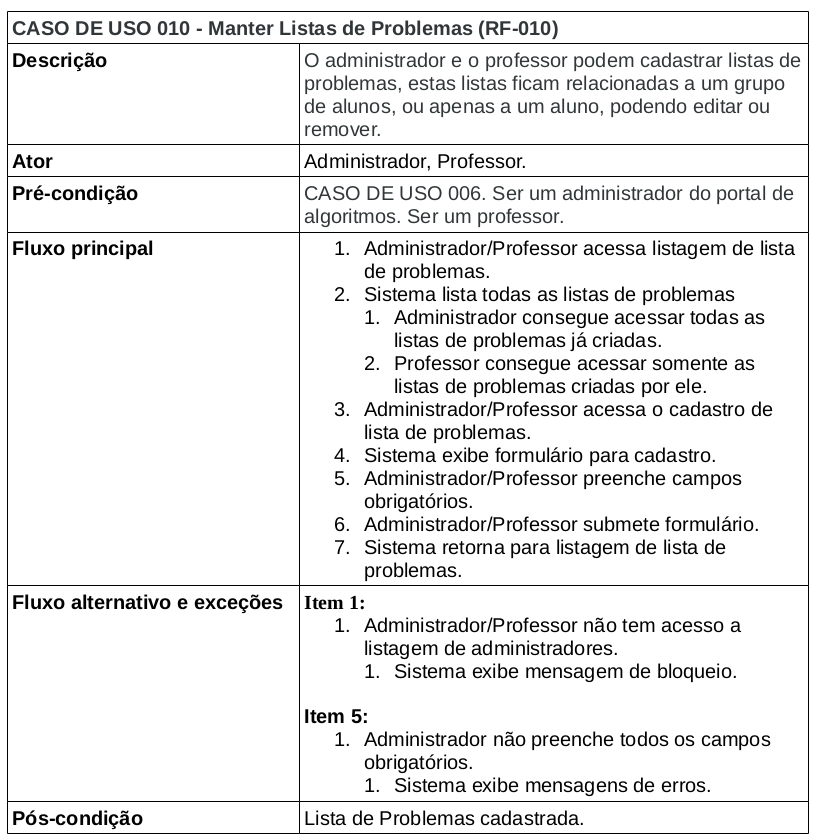
\includegraphics[width=15cm]{UML/casos-de-uso/10.png}
	\label{imgManterListaProblemas}
	Fonte: (AUTOR, 2018)
\end{table}
\FloatBarrier

\newpage

\subsubsection{Manter Institui��es}

A Tabela \ref{imgManterInstituicoes} descreve o caso de uso de manter o cadastro, edi��o e remo��o das institui��es que podem ser utilizadas no cadastro do professor.

\FloatBarrier
\begin{table}[!htb]
	\centering
	\caption{Caso de Uso Manter Institui��es}
	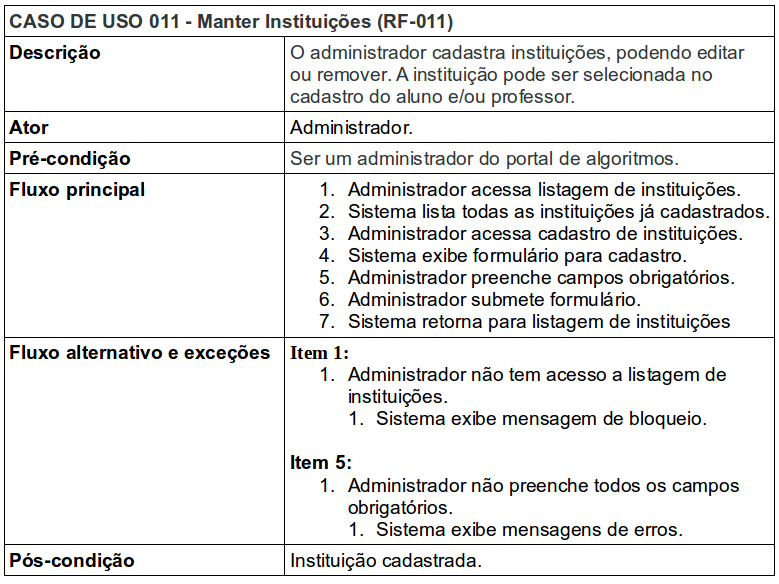
\includegraphics[width=15cm]{UML/casos-de-uso/11.png}
	\label{imgManterInstituicoes}
	Fonte: (AUTOR, 2018)
\end{table}
\FloatBarrier

\newpage

\subsubsection{Manter Grupos}

A Tabela \ref{imgManterGrupos} descreve o caso de uso de manter o cadastro, edi��o e remo��o de grupos. Os grupos servem para agrupar alunos e professores, onde o professores e administradores podem criar listas de problemas espec�ficos para os grupos ou alunos.

\FloatBarrier
\begin{table}[!htb]
	\centering
	\caption{Caso de Uso Manter Grupos}
	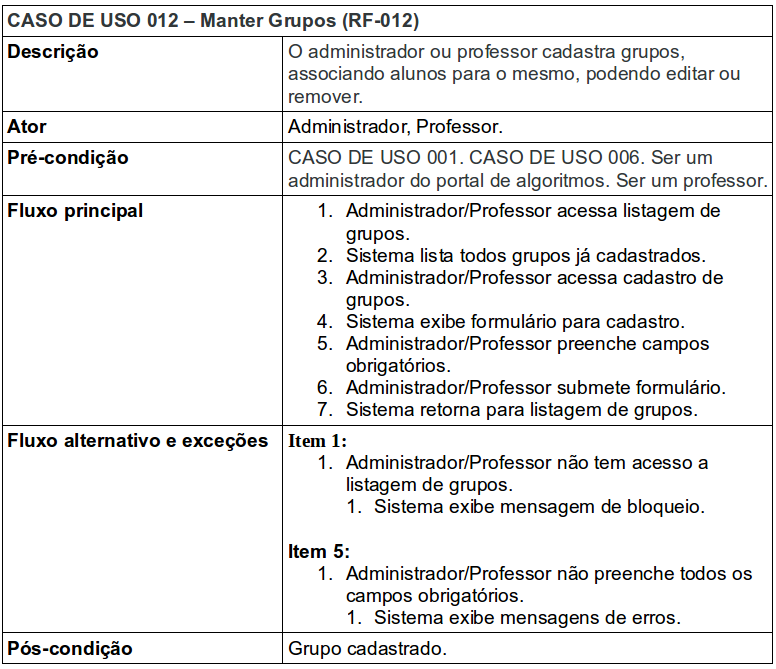
\includegraphics[width=15cm]{UML/casos-de-uso/12.png}
	\label{imgManterGrupos}
	Fonte: (AUTOR, 2018)
\end{table}
\FloatBarrier

\newpage

\subsubsection{Manter Permiss�es}

A Tabela \ref{imgManterPermissoes} descreve o caso de uso de manter o cadastro, edi��o e remo��o das permiss�es do portal de algoritmos. Essas permiss�es servem para permitir acesso a determinados cadastros do sistema.

\FloatBarrier
\begin{table}[!htb]
	\centering
	\caption{Caso de Uso Manter Permiss�es}
	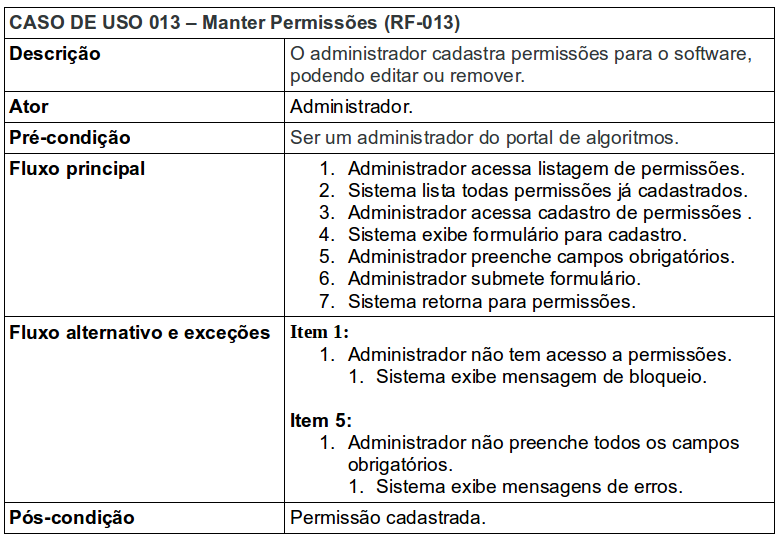
\includegraphics[width=15cm]{UML/casos-de-uso/13.png}
	\label{imgManterPermissoes}
	Fonte: (AUTOR, 2018)
\end{table}
\FloatBarrier

\newpage

\subsubsection{Manter Grupos de Administradores}

A Tabela \ref{imgManterGruposAdministradores} descreve o caso de uso de manter o cadastro, edi��o e remo��o de grupos de administradores. � um agrupador de usu�rios que tem a permiss�o de acessar o gerenciamento do portal de algoritmos.

\FloatBarrier
\begin{table}[!htb]
	\centering
	\caption{Caso de Uso Manter Grupos de Administradores}
	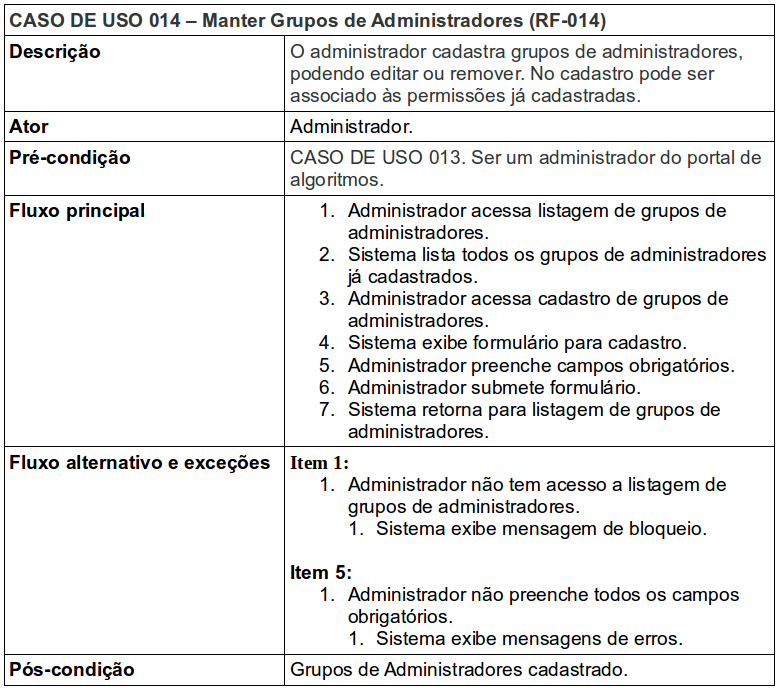
\includegraphics[width=15cm]{UML/casos-de-uso/14.png}
	\label{imgManterGruposAdministradores}
	Fonte: (AUTOR, 2018)
\end{table}
\FloatBarrier

\newpage

\subsubsection{Manter Pa�ses}

A Tabela \ref{imgManterPaises} descreve o caso de uso de manter  o cadastro, edi��o e remo��o de pa�ses.

\FloatBarrier
\begin{table}[!htb]
	\centering
	\caption{Caso de Uso Manter Pa�ses}
	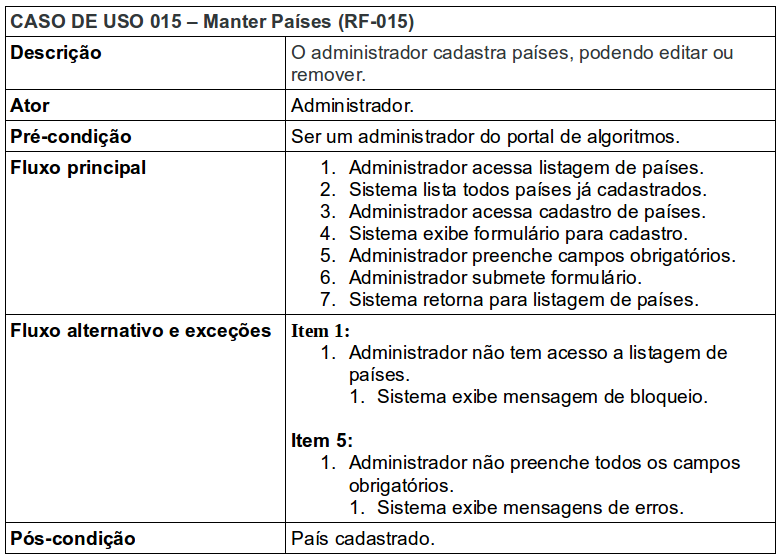
\includegraphics[width=15cm]{UML/casos-de-uso/15.png}
	\label{imgManterPaises}
	Fonte: (AUTOR, 2018)
\end{table}
\FloatBarrier

\newpage

\subsubsection{Manter Estados}

A Tabela \ref{imgManterEstados} descreve o caso de uso de manter  o cadastro, edi��o e remo��o de estados.

\FloatBarrier
\begin{table}[!htb]
	\centering
	\caption{Caso de Uso Manter Estados}
	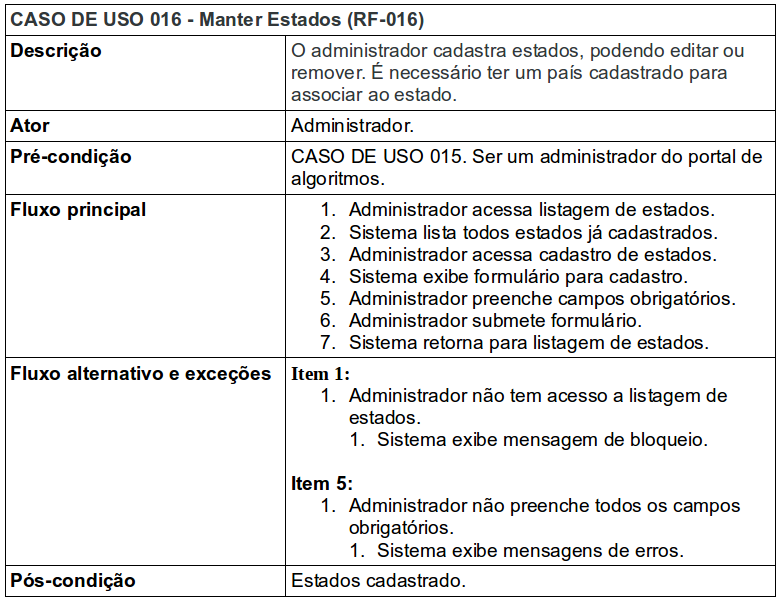
\includegraphics[width=15cm]{UML/casos-de-uso/16.png}
	\label{imgManterEstados}
	Fonte: (AUTOR, 2018)
\end{table}
\FloatBarrier

\newpage

\subsubsection{Manter Cidades}

A Tabela \ref{imgManterCidades} descreve o caso de uso de manter  o cadastro, edi��o e remo��o de cidades.

\FloatBarrier
\begin{table}[!htb]
	\centering
	\caption{Caso de Uso Manter Cidades}
	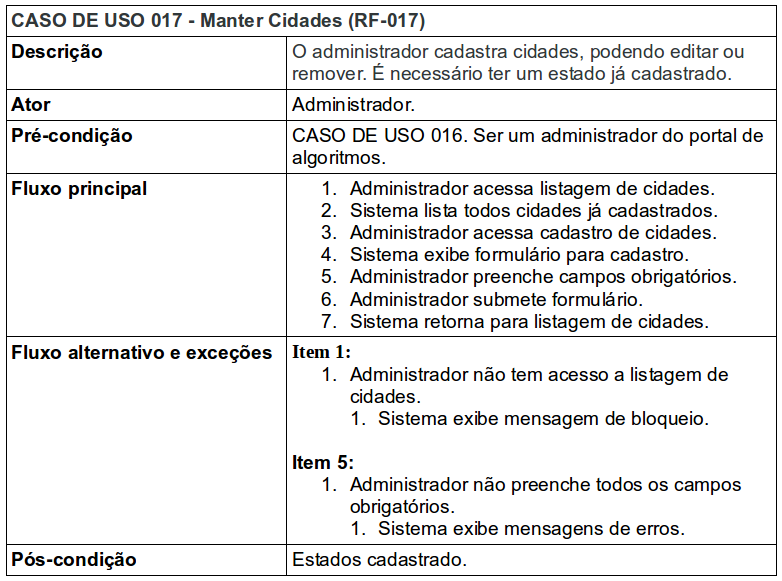
\includegraphics[width=15cm]{UML/casos-de-uso/17.png}
	\label{imgManterCidades}
	Fonte: (AUTOR, 2018)
\end{table}
\FloatBarrier

\newpage

\subsubsection{Manter suas Informa��es Pessoais}

A Tabela \ref{imgManterPerfil} descreve o caso de uso de cadastro, edi��o e remo��o das informa��es pessoais do aluno.

\FloatBarrier
\begin{table}[!htb]
	\centering
	\caption{Caso de Uso Aluno Manter suas Informa��es Pessoais}
	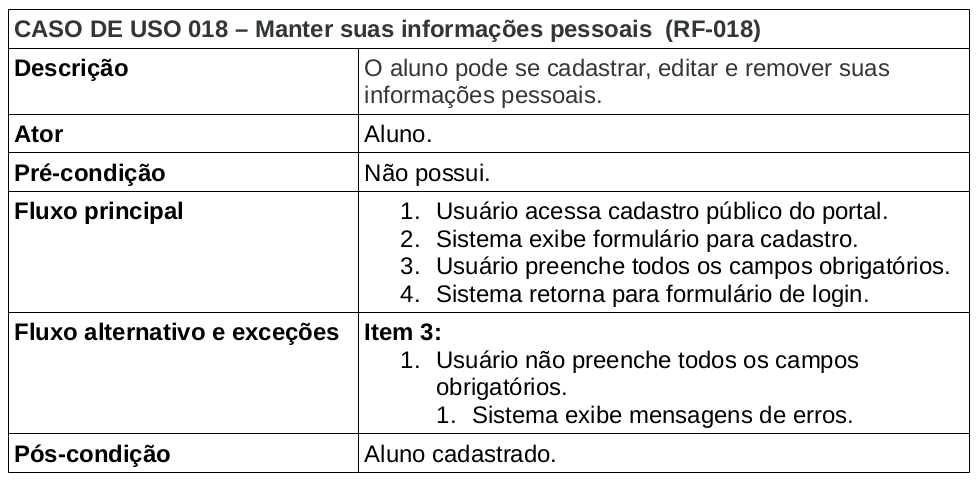
\includegraphics[width=15cm]{UML/casos-de-uso/19.png}
	\label{imgManterPerfil}
	Fonte: (AUTOR, 2018)
\end{table}
\FloatBarrier

Foram apresentados os casos de uso que ser�o utilizados para a evolu��o do portal de algoritmos. Na pr�xima Se��o ser�o apresentados os prot�tipos de interface do portal de algoritmos.

\newpage

\section{Interfaces Gr�ficas}\label{scPrototipos}

Os prot�tipos exibidos nessa se��o procuram seguir os seguintes princ�pios de usabilidade conforme \citet{Benyon2011}:

\begin{enumerate}
	\item Visibilidade: garante que os elementos sejam vis�veis, de forma que as pessoas possam ver quais fun��es est�o dispon�veis e o que o sistema est� fazendo atualmente.
	\item Consist�ncia: mant�m consist�ncia no uso de caracter�sticas de \textit{design} e com sistema semelhantes e m�todo-padr�o de trabalho.
	\item Familiaridade: utiliza linguagem e s�mbolos com os quais os futuros usu�rios est�o familiarizados.
	\item \textit{Affordance}: criar \textit{design} de forma que fique claro para o qu� elas servem.
	\item Navega��o: proporcione suporte para que as pessoas possam se movimentar pelo sistema.
	\item Retorno: retorna as informa��es rapidamente a informa��o do sistema para os usu�rios para que elas saibam que efeito suas a��es causaram.
	\item Estilo: \textit{designs} devem ser elegantes e atraentes.
\end{enumerate}

\newpage

\subsection{Cadastro de Aluno}

A Figura \ref{mkCadastroAluno} � a interface gr�fica de cadastro de um novo aluno.

\FloatBarrier
\begin{figure}[!htb]
	\centering
	\caption{Interface Gr�fica de Cadastro de Aluno}
	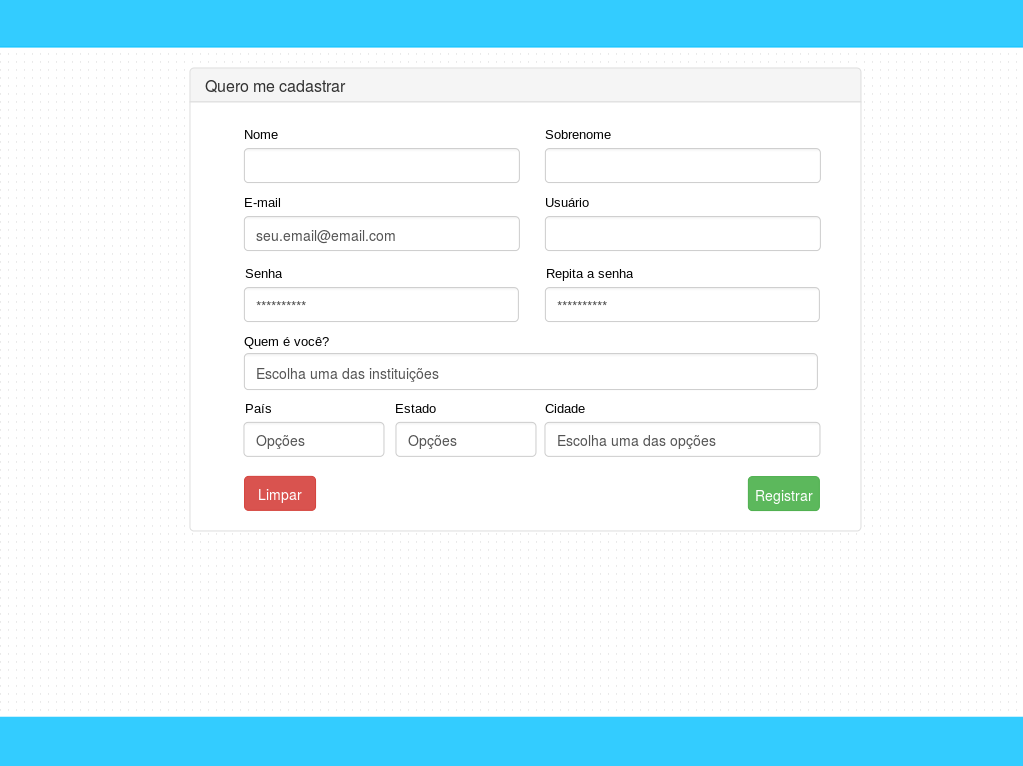
\includegraphics[width=15cm]{mockups/1.png}
	\label{mkCadastroAluno}
	Fonte: (AUTOR, 2018)
\end{figure}
\FloatBarrier

Nessa interface gr�fica o aluno preenche todos os campos abaixo:

\begin{itemize}
	\item Nome.
	\item Sobrenome.
	\item E-mail.
	\item Login: o login � seu \textit{username} que ser� utilizado para acessar o portal de algoritmos.
	\item Senha.
	\item Repita a senha: nesse campo faz-se a verifica��o se a senha digitada anteriormente corresponde a essa.
	\item Institui��o: exibe todas institui��es cadastradas pelo administrador.
	\item Cidade: exibe todas cidades cadastradas pelo administrador.
\end{itemize}

Ap�s o preenchimento de todos os campos, o alunos clica em ``Salvar" \ e seu cadastro estar� realizado.

\newpage

\subsection{Autentica��o}

A Figura \ref{mkAutenticacao} � ainterface gr�fica de autentica��o.

\FloatBarrier
\begin{figure}[!htb]
	\centering
	\caption{Interface Gr�fica de Autentica��o}
	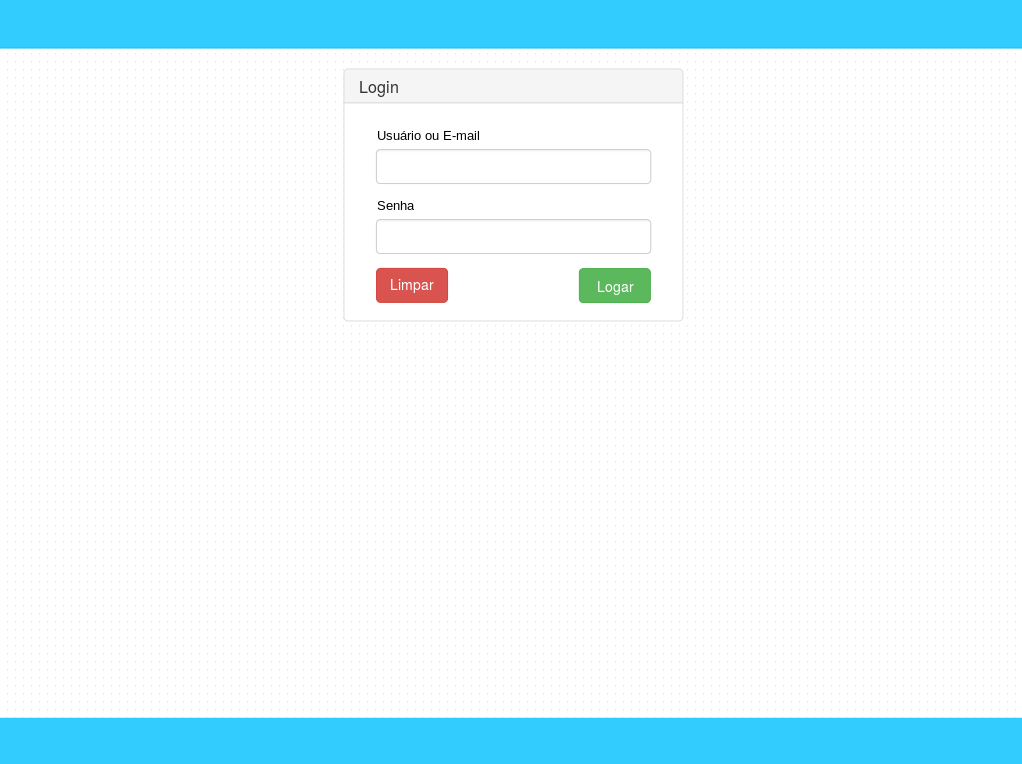
\includegraphics[width=15cm]{mockups/5.png}
	\label{mkAutenticacao}
	Fonte: (AUTOR, 2018)
\end{figure}
\FloatBarrier

Nessa interface gr�fica o aluno, professor ou administrador realiza a autentica��o no portal de algoritmos. A autentica��o somente � autorizada para usu�rios ainda ativos no sistema.

O seu funcionamento � simples, o usu�rio preenche os campos de ``Usu�rio ou E-mail" \  e ``Senha" \  com as seguintes informa��es, e-mail ou usu�rio e senha, o usu�rio estando ativo no sistema ele ser� redirecionado para a p�gina inicial do sistema.

\newpage

\subsection{Boas Vindas ao Administrador e Professor}

A Figura \ref{mkBoasVindasAdministrador} � ainterface gr�fica de Boas Vindas do Administrador e Professor.

\FloatBarrier
\begin{figure}[!htb]
	\centering
	\caption{Interface Gr�fica de Boas Vindas do Administrador e Professor}
	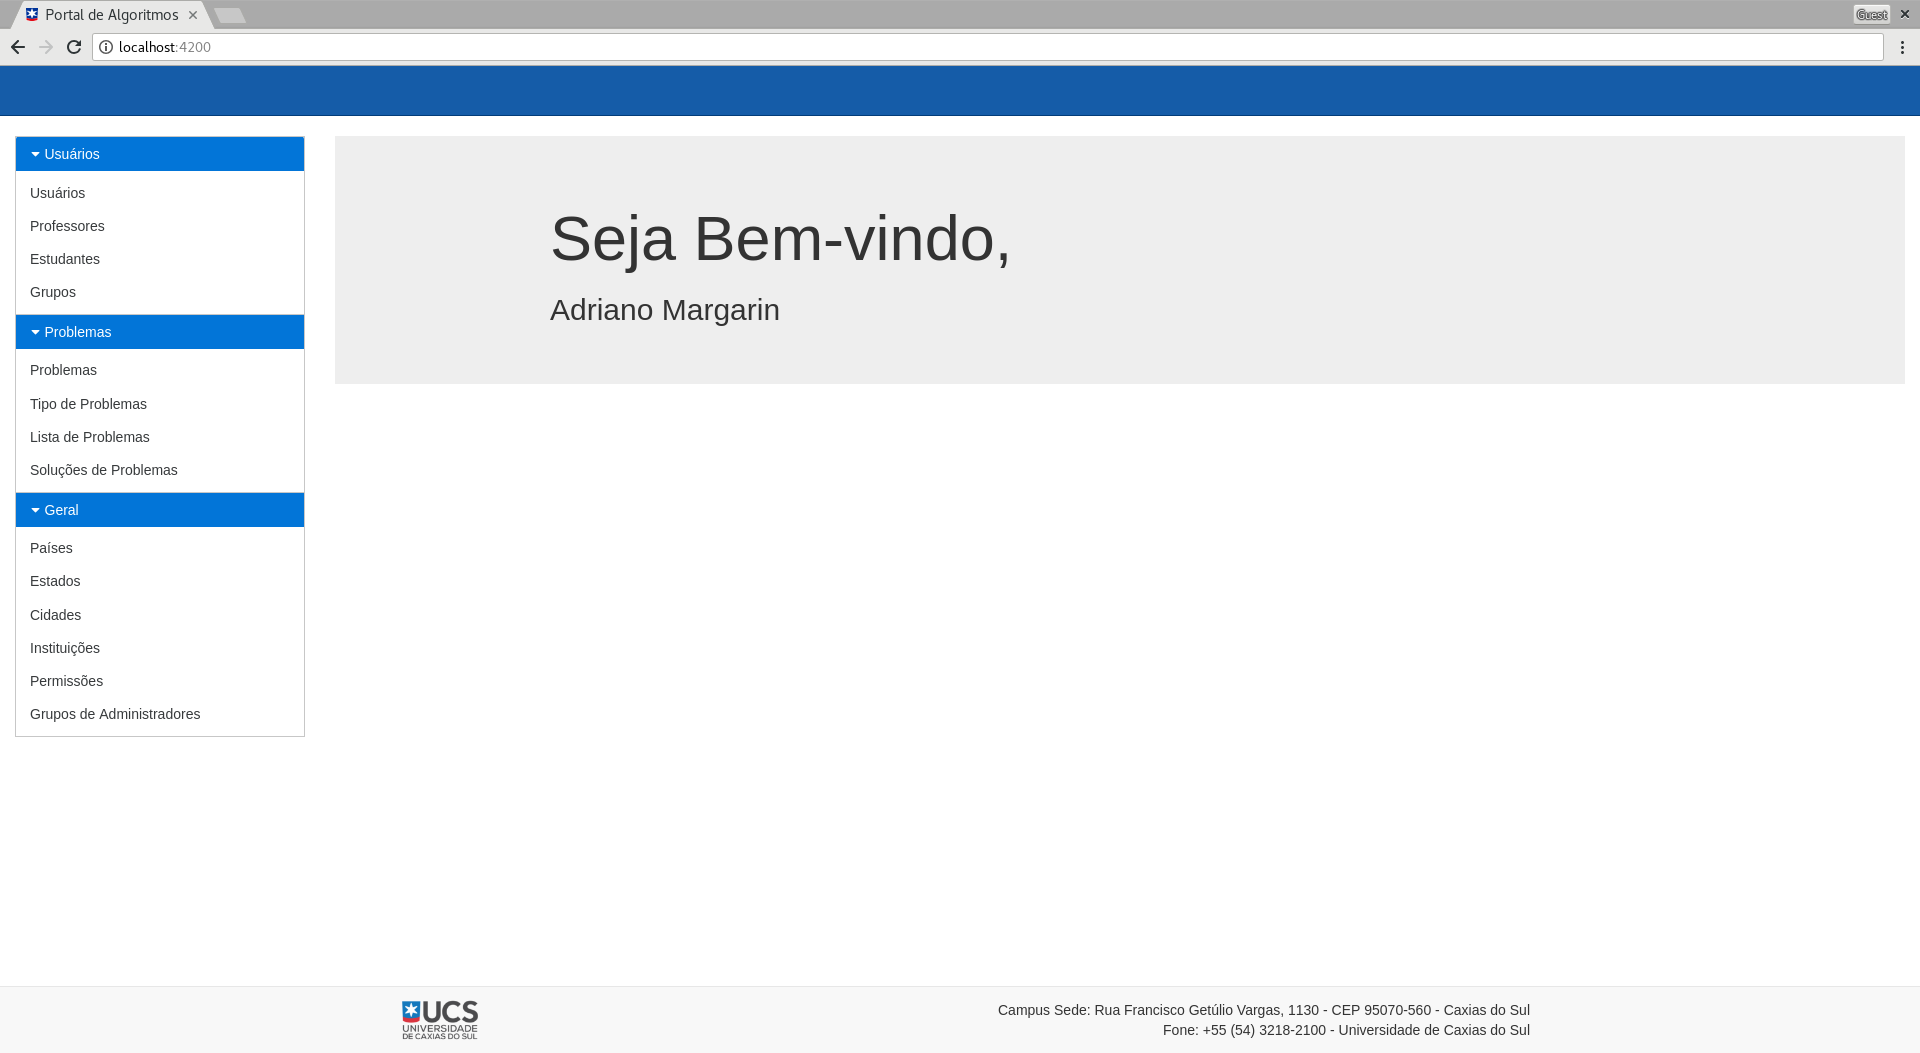
\includegraphics[width=15cm]{mockups/3.png}
	\label{mkBoasVindasAdministrador}
	Fonte: (AUTOR, 2018)
\end{figure}
\FloatBarrier

Essa interface gr�fica � exibida ap�s a autentica��o com sucesso do Administrador ou Professor. Nessa interface � exibida uma �rvore com links para as demais interfaces gr�ficas, agrupadas por contextos.

\newpage

\subsection{Problemas}\label{scListaProblemas}

A Figura \ref{mkListaProblemas} � a interface gr�fica da listagem de problemas. 

\FloatBarrier
\begin{figure}[!htb]
	\centering
	\caption{Interface Gr�fica de Problemas}
	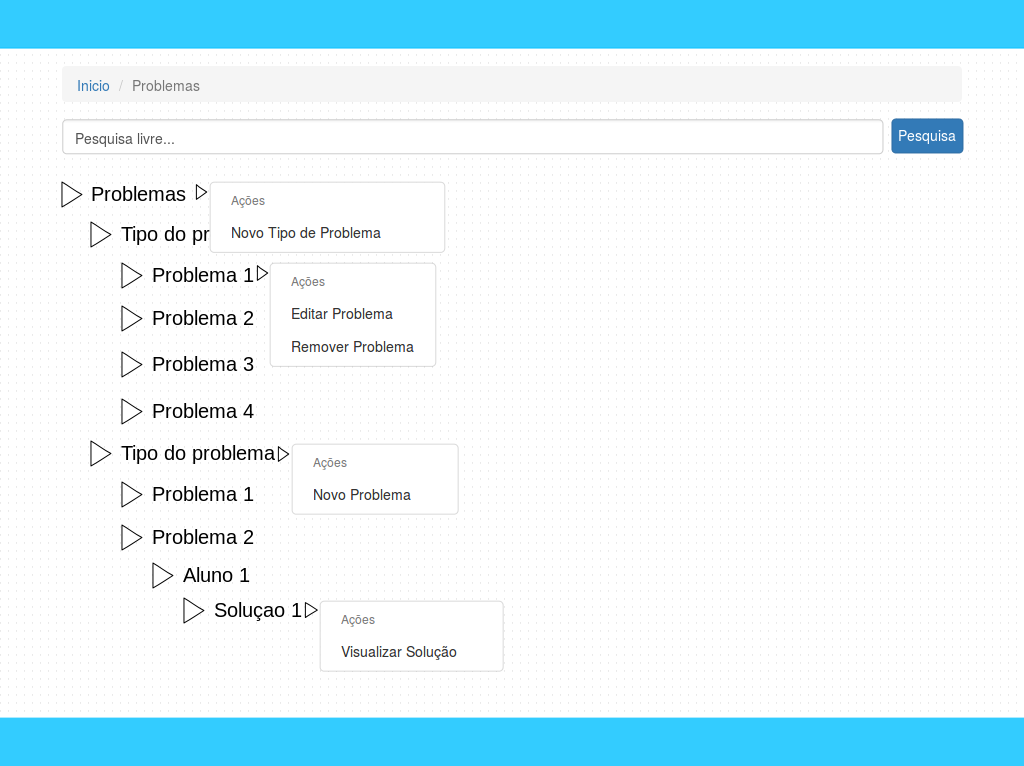
\includegraphics[width=15cm]{mockups/6.png}
	\label{mkListaProblemas}
	Fonte: (AUTOR, 2018)
\end{figure}
\FloatBarrier

Essa interface gr�fica possui as seguintes a��es:

\begin{itemize}
	\item Pesquisa livre.
	\begin{itemize}
		\item O administrador pode realizar a filtragem por qualquer palavra.
	\end{itemize}
	\item Novo Tipo de Problema.
	\begin{itemize}
		\item Selecionando essa a��o, o administrador � direcionado para a interface gr�fica da Figura \ref{mkNovoTipoProblema}.
	\end{itemize}
	\item Novo Problema.
	\begin{itemize}
		\item Selecionando essa a��o, o adminsitrador � direcionado para a interface gr�fica da Figura \ref{mkNovoProblema}.
	\end{itemize}
	\item Editar Problema.
	\begin{itemize}
		\item Selecionando essa a��o, o administrador � direcionado para a interface gr�fica da Figura \ref{mkNovoProblema}.
	\end{itemize}
	\item Remover Problema.
	\begin{itemize}
		\item Selecionando essa a��o, o administrador remove o problema.
	\end{itemize}
\end{itemize}

\newpage

\subsection{Tipo de Problema}

A Figura \ref{mkNovoTipoProblema} � a interface gr�fica de listagem de tipos de problemas.

\FloatBarrier
\begin{figure}[!htb]
	\centering
	\caption{Interface Gr�fica de Listagem Tipos de Problemas}
	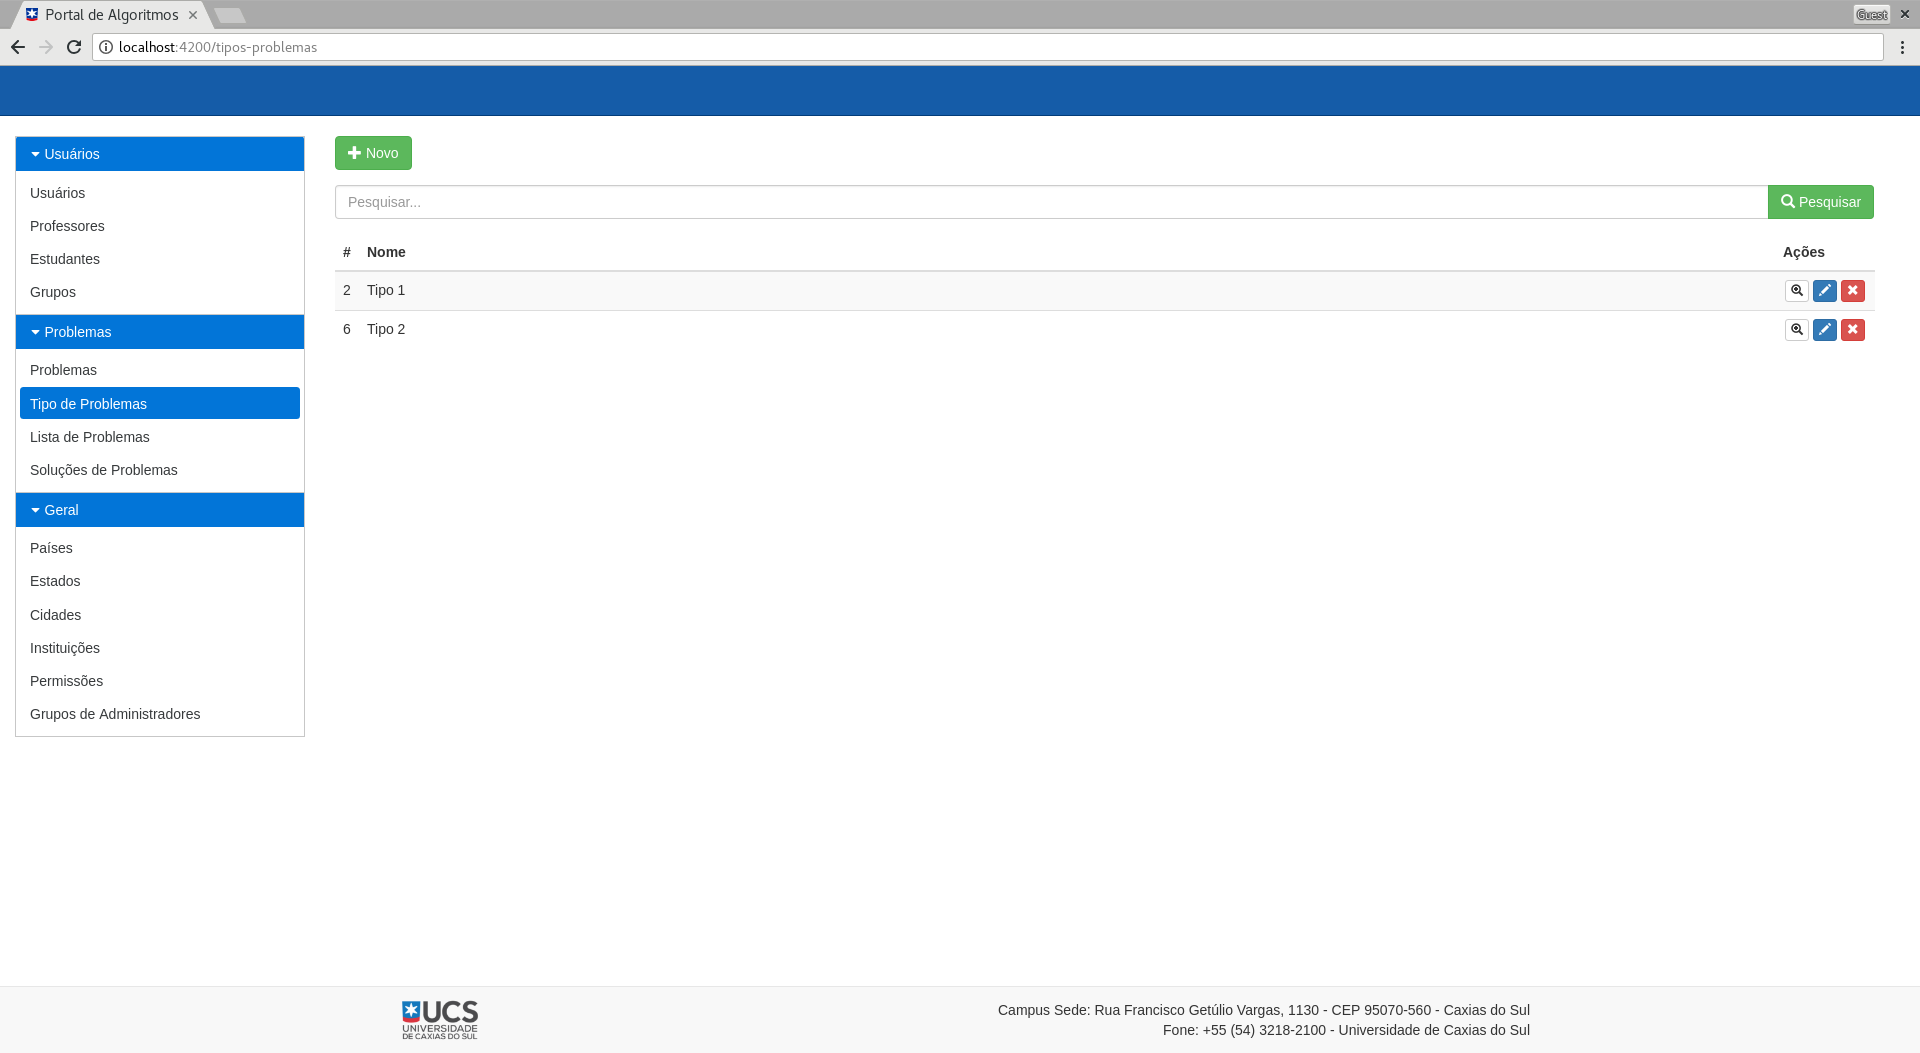
\includegraphics[width=15cm]{mockups/7.png}
	\label{mkNovoTipoProblema}
	Fonte: (AUTOR, 2018)
\end{figure}
\FloatBarrier

Nessa interface gr�fica o administrador visualiza todas os Tipos de Problemas j� cadastrados, podendo adicionar, editar e remover.

\newpage

\subsection{Cadastro e Edi��o de Problema}

A Figura \ref{mkNovoProblema} � a interface gr�fica de cadastro e/ou edi��o de um novo problema.

\FloatBarrier
\begin{figure}[!htb]
	\centering
	\caption{Interface Gr�fica de Novo Problema}
	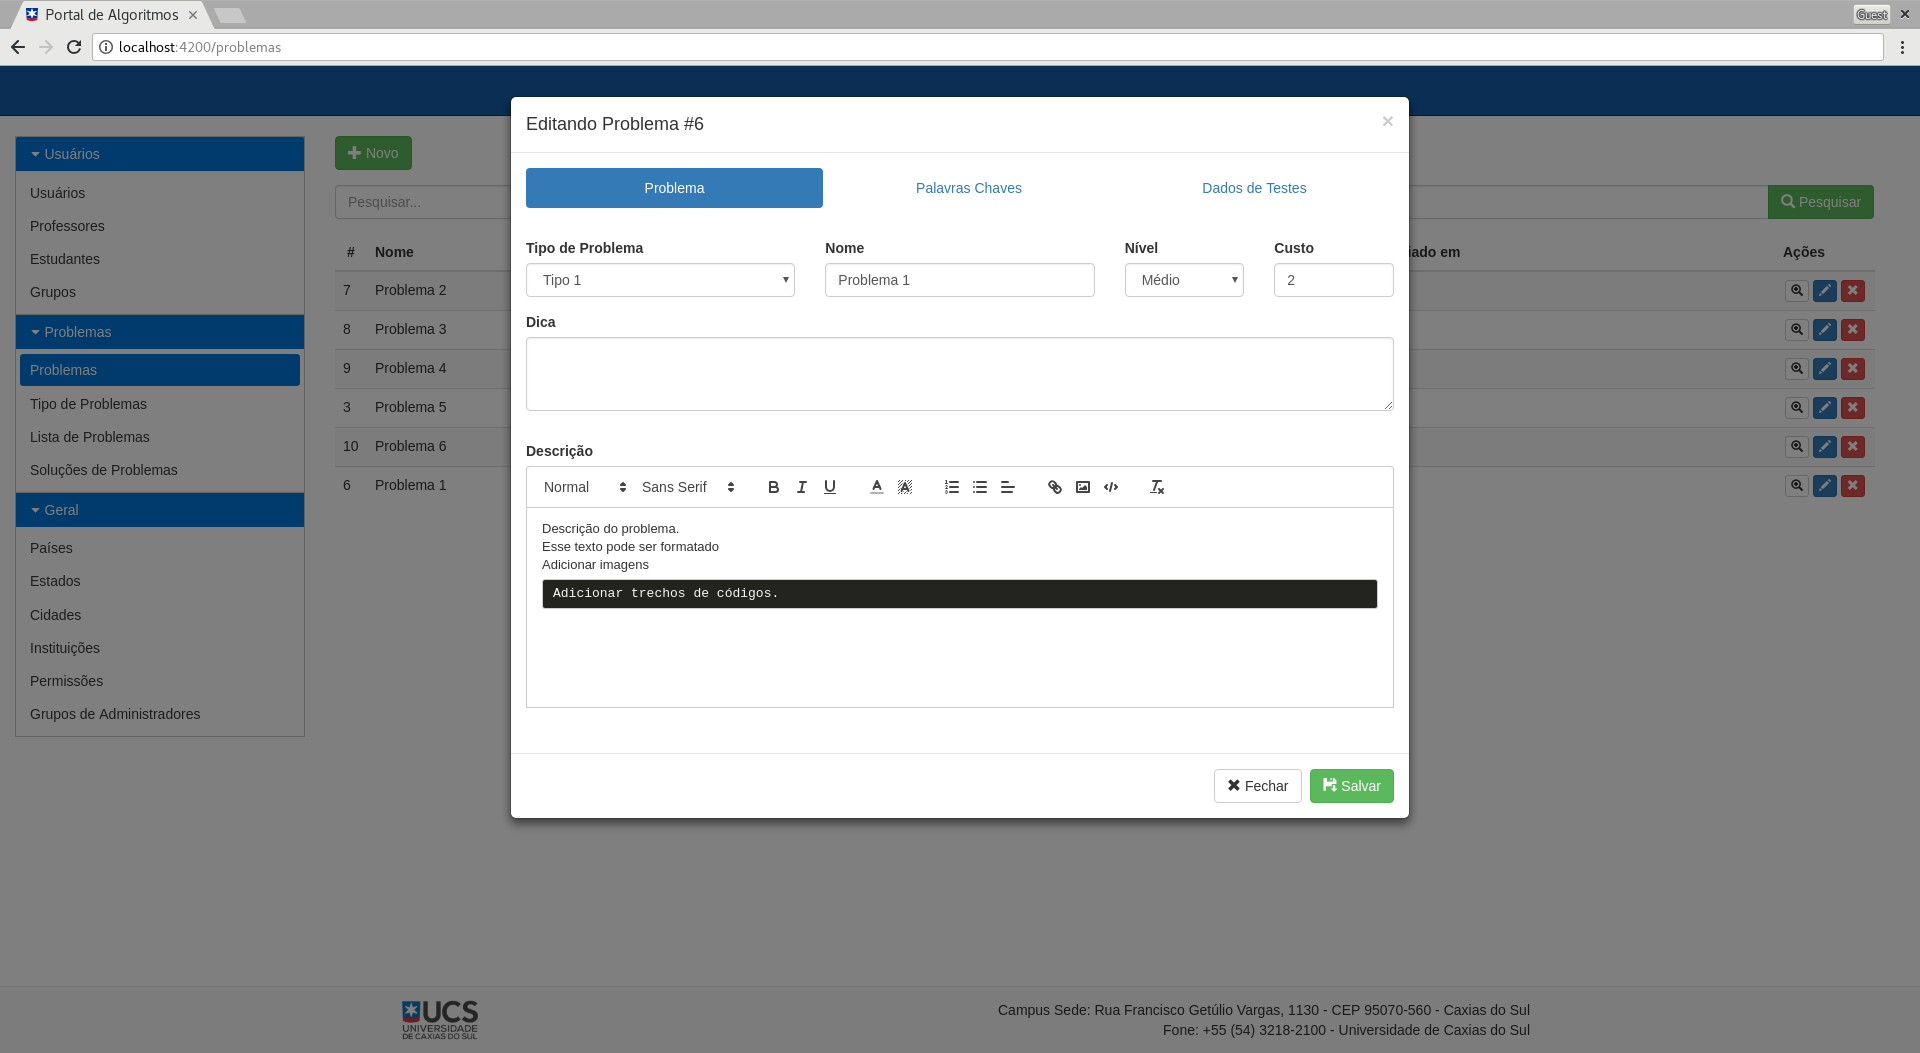
\includegraphics[width=15cm]{mockups/8.png}
	\label{mkNovoProblema}
	Fonte: (AUTOR, 2018)
\end{figure}
\FloatBarrier

A interface est� dividida em tr�s abas, Problema, Palavras Chave e Dados de Testes, cada uma dessas abas est�o descritas abaixo:

\begin{itemize}
	\item Problema.
	\begin{itemize}
		\item O cadastro ou edi��o do problema consiste em preencher os campos, ``Tipo de Problema", ``Nome do Problema", ``Dica" \ e ``N�vel", o ``Custo" \ � correspondente ao menor custo de alguma solu��o daquele problema.
	\end{itemize}
	\item Palavras Chaves.
	\begin{itemize}
		\item O cadastro de palavras-chave � descrito na Se��o \ref{scPalavraChave}
	\end{itemize}
	\item Dados de Testes.
	\begin{itemize}
		\item O cadastro de dados de testes � descrito na Se��o \ref{scDadosTestes}
	\end{itemize}
\end{itemize}

Toda a a��o nessa interface deve ser gravada ao clicar no bot�o ``Salvar".

\subsection{Palavras-chave}\label{scPalavraChave}

A Figura \ref{mkPalavrasChaves} � a interface gr�fica de cadastro e/ou edi��o de palavras-chave de um problema.

\FloatBarrier
\begin{figure}[!htb]
	\centering
	\caption{Interface Gr�fica de Palavras Chaves}
	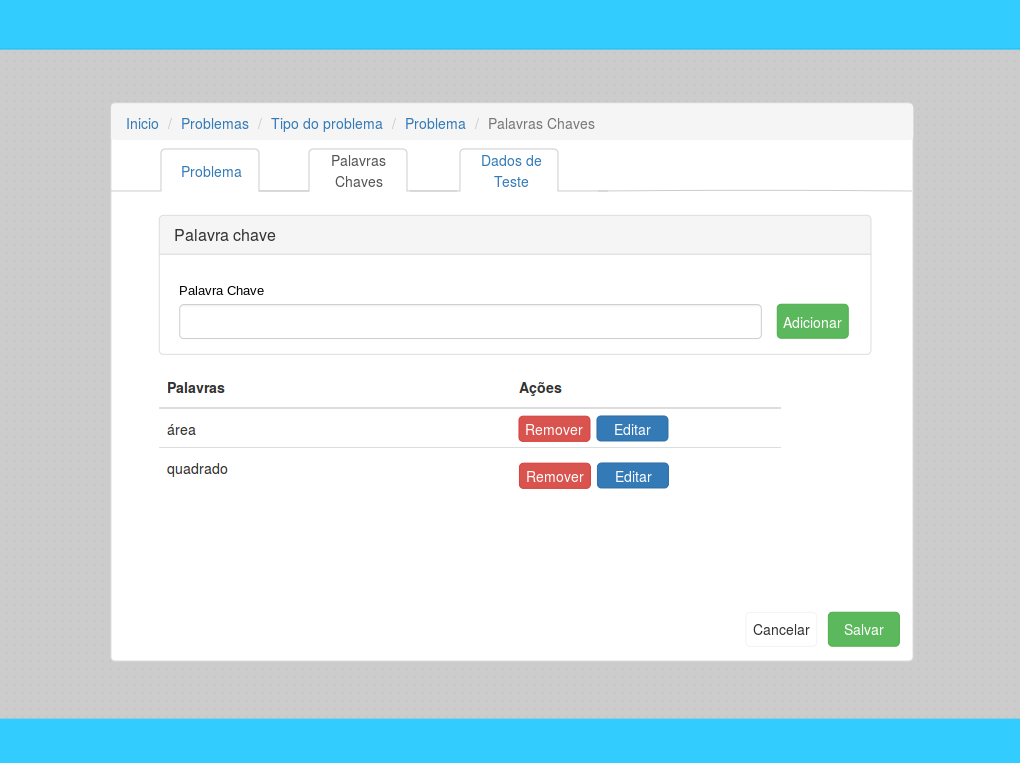
\includegraphics[width=15cm]{mockups/9.png}
	\label{mkPalavrasChaves}
	Fonte: (AUTOR, 2018)
\end{figure}
\FloatBarrier

Nessa interface o administrador preenche o campo ``Palavra-chave" \  e clica em ``Adicionar". Fazendo essa a��o ele associa a nova palavra-chave ao problema que ele est� cadastrando ou editando. O administrador pode tamb�m editar ou remover uma palavra-chave j� cadastrada, para isso � preciso selecionar um das a��es, ``Editar" \ ou ``Remover".

\newpage

\subsection{Dados de Testes}\label{scDadosTestes}

A Figura \ref{mkDadosTestes} � a interface gr�fica de cadastro e/ou edi��o de dados de testes de um problema.

\FloatBarrier
\begin{figure}[!htb]
	\centering
	\caption{Interface Gr�fica de Dados de Testes}
	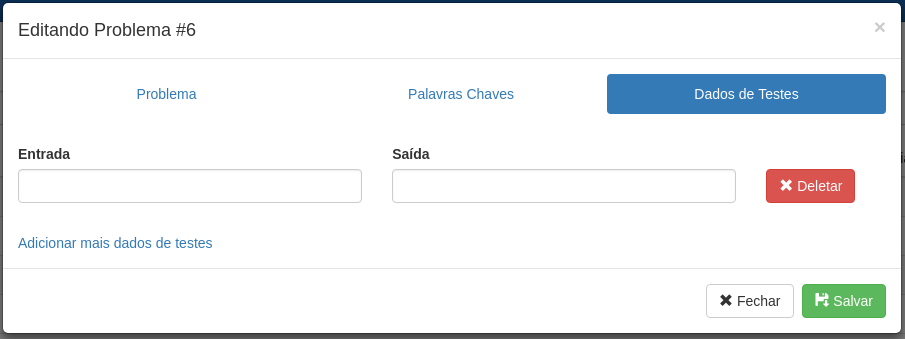
\includegraphics[width=15cm]{mockups/10.png}
	\label{mkDadosTestes}
	Fonte: (AUTOR, 2018)
\end{figure}
\FloatBarrier

Nessa interface o administrador preenche os campos ``Entrada" \ e ``Sa�da" \  e clica em ``Adicionar", fazendo essa a��o ele associa o novo dado de teste ao problema que ele est� cadastrando ou editando. O administrador pode tamb�m editar ou remover um dado de teste j� cadastrado, para isso � preciso selecionar um das a��es, ``Editar" \  ou ``Remover". Um problema pode ter apenas dados de testes de ``Entrada" \ ou somente de ``Sa�da".


\newpage

\subsection{Visualiza��o de Solu��o de Problema}

A Figura \ref{mkVisualizacaoSolucao1} � a interface gr�fica de visualiza��o de uma solu��o de um problema.

\FloatBarrier
\begin{figure}[!htb]
	\centering
	\caption{Interface Gr�fica de Visualiza��o de Solu��o do Problema}
	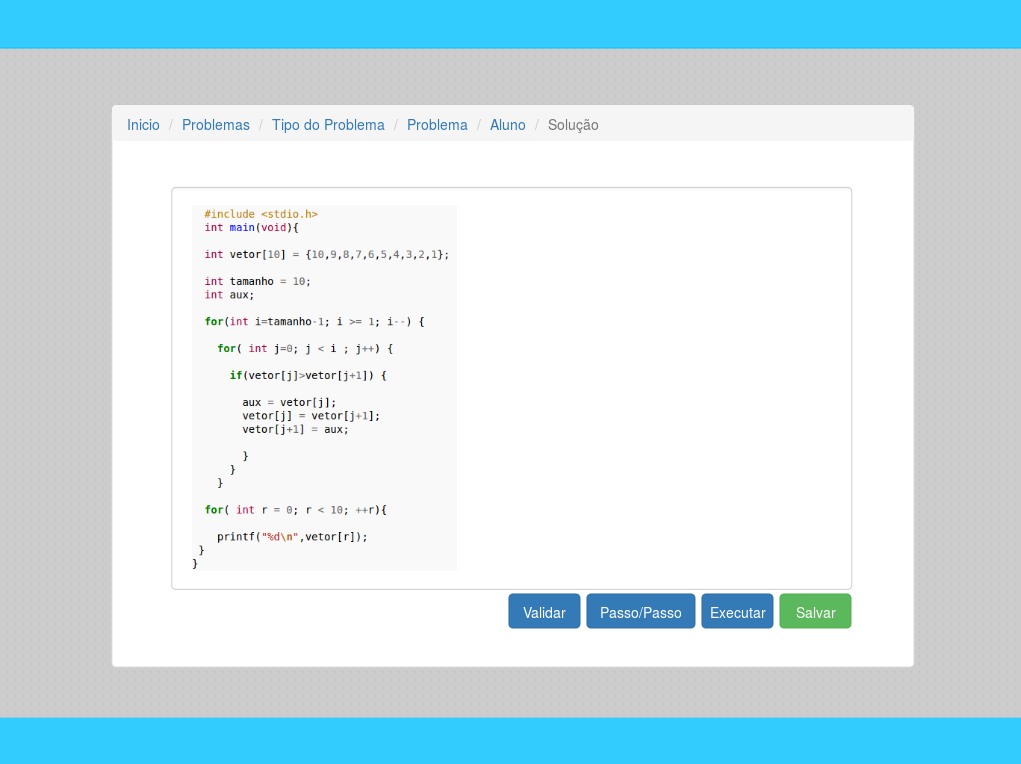
\includegraphics[width=15cm]{mockups/11.png}
	\label{mkVisualizacaoSolucao1}
	Fonte: (AUTOR, 2018)
\end{figure}
\FloatBarrier
\newpage

\subsection{Lista de Grupos}

A Figura \ref{mkListaGrupos} � a interface gr�fica de listagem dos grupos j� cadastrados. Essa listagem corresponde a todos os grupos, caso seja um administrador com total acesso, ou apenas aos grupos cadastrados por um professor, sendo que o professor somente ter� na listagem os grupos que ele cadastrou.

\FloatBarrier
\begin{figure}[!htb]
	\centering
	\caption{Interface Gr�fica de Grupos}
	\includegraphics[width=15cm]{mockups/12.png}
	\label{mkListaGrupos}
	Fonte: (AUTOR, 2018)
\end{figure}
\FloatBarrier

Nessa interface gr�fica possu�mos as seguintes a��es:

\begin{itemize}
	\item Pesquisa Livre.
	\begin{itemize}
		\item O administrador pode realizar a pesquisa por qualquer palavra.
	\end{itemize}
	\item Novo Grupo.
	\begin{itemize}
		\item Selecionando essa a��o, o administrador � direcionado para a interface gr�fica da Figura \ref{mkCadastroGrupo}
	\end{itemize}
	\item Editar Grupo.
	\begin{itemize}
		\item Selecionando essa a��o, o administrador � direcionado para a interface gr�fica da Figura \ref{mkCadastroGrupo}
	\end{itemize}
	\item Remover Grupo.
	\begin{itemize}
		\item Selecionando essa a��o, o administrador remove somente o grupo, sendo assim, n�o remove problemas, solu��es e/ou usu�rios.
	\end{itemize}
\end{itemize}

\newpage

\subsection{Cadastro e Edi��o de Grupo}

A Figura \ref{mkCadastroGrupo} � a interface gr�fica de cadastro e edi��o de um grupo.

\FloatBarrier
\begin{figure}[!htb]
	\centering
	\caption{Interface Gr�fica de Cadastro de Grupo}
	\includegraphics[width=15cm]{mockups/13.png}
	\label{mkCadastroGrupo}
	Fonte: (AUTOR, 2018)
\end{figure}
\FloatBarrier

A interface gr�fica est� dividida em tr�s abas, Grupo, Participantes, Lista de Problemas sendo que cada uma dessas abas est�o descritas abaixo:

\begin{itemize}
	\item Grupo.
	\begin{itemize}
		\item Para o cadastro de um novo grupo, basta preencher os campos, Nome e Descri��o.
	\end{itemize}
\end{itemize}

\newpage

\subsection{Adicionar Participantes}

A Figura \ref{mkParticipantes} � a interface gr�fica de associa��o de participantes em um grupo.

\FloatBarrier
\begin{figure}[!htb]
	\centering
	\caption{Interface Gr�fica de Cadastro de Participantes no Grupo}
	\includegraphics[width=15cm]{mockups/14.png}
	\label{mkParticipantes}
	Fonte: (AUTOR, 2018)
\end{figure}
\FloatBarrier

Utilizando os bot�es centrais, � poss�vel adicionar ou remover participantes, podendo-se adicionar ou remover todos ou um e/ou mais por vez.

\newpage

\subsection{Adicionar Lista de Problemas}

A Figura \ref{mkGrupoListaProblemas} � a interface gr�fica de associa��o de lista de problemas em um grupo.

\FloatBarrier
\begin{figure}[!htb]
	\centering
	\caption{Interface Gr�fica de Cadastro de Lista de Problemas no Grupo}
	\includegraphics[width=15cm]{mockups/15.png}
	\label{mkGrupoListaProblemas}
	Fonte: (AUTOR, 2018)
\end{figure}
\FloatBarrier

Utilizando os bot�es centrais, � poss�vel adicionar ou remover listas de problemas, podendo-se adicionar ou remover todos ou um e/ou mais por vez.

\newpage

\subsection{Lista de Alunos}

A Figura \ref{mkListaAlunos} � a interface gr�fica da listagem de alunos.

\FloatBarrier
\begin{figure}[!htb]
	\centering
	\caption{Interface Gr�fica de Listagem de Alunos}
	\includegraphics[width=15cm]{mockups/17.png}
	\label{mkListaAlunos}
	Fonte: (AUTOR, 2018)
\end{figure}
\FloatBarrier

Nessa interface gr�fica encontramos as seguintes a��es:

\begin{itemize}
	\item Pesquisa Livre: o administrador pode realizar a pesquisa por qualquer palavra.
	\item Novo Aluno: selecionando essa a��o, o administrador � direcionado para a interface gr�fica da Figura \ref{mkCadastroAlunoAdmin}
	\item Editar Aluno: selecionando essa a��o, o administrador � direcionado para a interface gr�fica da Figura \ref{mkCadastroAlunoAdmin}
	\item Remover Aluno: selecionando essa a��o, o administrador remove o aluno.
\end{itemize}

\newpage

\subsection{Cadastro de Alunos}

A Figura \ref{mkCadastroAlunoAdmin} � a interface gr�fica do cadastro e edi��o de alunos.

\FloatBarrier
\begin{figure}[!htb]
	\centering
	\caption{Interface Gr�fica de Cadastro de Alunos}
	\includegraphics[width=15cm]{mockups/38.png}
	\label{mkCadastroAlunoAdmin}
	Fonte: (AUTOR, 2018)
\end{figure}
\FloatBarrier

A �nica informa��o que � necess�rio preencher � selecionar um Usu�rio sendo que esse usu�rio ficar� associado ao cadastro do aluno.

\newpage

\subsection{Listas de Problemas}

A Figura \ref{mkListaProblemasListagem} � a interface da listagem de listas de problemas. Essa interface apresenta todas as listas de problemas j� cadastradas no portal de algoritmos.

\FloatBarrier
\begin{figure}[!htb]
	\centering
	\caption{Interface Gr�fica de Lista de Problemas}
	\includegraphics[width=15cm]{mockups/23.png}
	\label{mkListaProblemasListagem}
	Fonte: (AUTOR, 2018)
\end{figure}
\FloatBarrier

Nessa interface gr�fica temos as seguintes a��es:

\begin{itemize}
	\item Pesquisa Livre: o administrador pode realizar a pesquisa por qualquer palavra.
	\item Nova Lista: selecionado essa a��o, o administrador � direcionado para a interface gr�fica da Figura \ref{mkCadastroListaProblemas}
	\item Editar Lista: selecionado essa a��o, o administrador � direcionado para a interface gr�fica da Figura \ref{mkCadastroListaProblemas}
	\item Remover Lista: selecionando essa a��o, o administrador remove uma lista.
\end{itemize}

\newpage

\subsection{Cadastro e Edi��o de Lista de Problemas}

A Figura \ref{mkCadastroListaProblemas} � a interface de cadastro e edi��o de lista de problemas.

\FloatBarrier
\begin{figure}[!htb]
	\centering
	\caption{Interface Gr�fica de Cadastro e Edi��o de Lista de Problemas}
	\includegraphics[width=15cm]{mockups/25.png}
	\label{mkCadastroListaProblemas}
	Fonte: (AUTOR, 2018)
\end{figure}
\FloatBarrier

Para cadastrar ou editar, o administrador deve preencher um nome para lista e selecionar os problemas conforme as a��es dispon�veis na interface.

\newpage

\subsection{Lista de Usu�rios}

A Figura \ref{mkListaUsuario} � a interface gr�fica da listagem dos usu�rios. Essa interface lista todos os usu�rios cadastrados no portal de algoritmos, incluindo os inativos.

\FloatBarrier
\begin{figure}[!htb]
	\centering
	\caption{Interface Gr�fica de Lista de Usu�rios}
	\includegraphics[width=15cm]{mockups/36.png}
	\label{mkListaUsuario}
	Fonte: (AUTOR, 2018)
\end{figure}
\FloatBarrier

Nessa interface gr�fica temos as seguintes a��es:

\begin{itemize}
	\item Pesquisa Livre: o administrador pode realizar a pesquisa por qualquer palavra.
	\item Novo Usu�rio: selecionando essa a��o, o administrador � direcionado para a interface gr�fica da Figura \ref{mkCadastroUsuario}.
	\item Editar Usu�rio: selecionando essa a��o, o administrador � direcionado para a interface gr�fica da Figura \ref{mkCadastroUsuario}.
	\item Remover Usu�rio: selecionando essa a��o, o administrador remove um usu�rio.
\end{itemize}

\newpage

\subsection{Cadastro e Edi��o de Usu�rios}

A Figura \ref{mkCadastroUsuario} � a interface gr�fica do cadastro e edi��o dos usu�rios.

\FloatBarrier
\begin{figure}[!htb]
	\centering
	\caption{Interface Gr�fica de Cadastro e Edi��o de Usu�rios}
	\includegraphics[width=15cm]{mockups/37.png}
	\label{mkCadastroUsuario}
	Fonte: (AUTOR, 2018)
\end{figure}
\FloatBarrier

O administrador preenche todos os campos do cadastro e clica em ``Salvar". Ap�s o administrador cadastrar ou editar o aluno o sistema retorna para listagem de usu�rios.

\newpage

\subsection{Lista de Professores}

A Figura \ref{mkListaProfessores} � a interface gr�fica da listagem dos professores.

\FloatBarrier
\begin{figure}[!htb]
	\centering
	\caption{Interface Gr�fica de Lista de Professores}
	\includegraphics[width=15cm]{mockups/28.png}
	\label{mkListaProfessores}
	Fonte: (AUTOR, 2018)
\end{figure}
\FloatBarrier

Nessa interface gr�fica temos as seguintes a��es:

\begin{itemize}
	\item Pesquisa Livre: o administrador pode realizar a pesquisa por qualquer palavra.
	\item Novo Professor: selecionando essa a��o, o administrador � direcionado para a interface gr�fica da Figura \ref{mkCadastroProfessores}.
	\item Editar Professor: selecionando essa a��o, o administrador � direcionado para a interface gr�fica da Figura \ref{mkCadastroProfessores}.
	\item Remover Professor: selecionando essa a��o, o administrador remove um Professor.
\end{itemize}

\newpage

\subsection{Cadastro e Edi��o de Professores}

A Figura \ref{mkCadastroProfessores} � a interface gr�fica do cadastro e edi��o dos professores.

\FloatBarrier
\begin{figure}[!htb]
	\centering
	\caption{Interface Gr�fica de Cadastro e Edi��o de Professores}
	\includegraphics[width=15cm]{mockups/29.png}
	\label{mkCadastroProfessores}
	Fonte: (AUTOR, 2018)
\end{figure}
\FloatBarrier

O administrador seleciona um usu�rio para cadastrar como professor, podendo tamb�m associar a institui��o que ele pertence. Ap�s preencher todo o cadastro, o administrador clica em ``Salvar" \ e o sistema direciona para listagem de professores.

\newpage

\subsection{Lista de Institui��es}

A Figura \ref{mkListaInstituicao} � a interface gr�fica da listagem das Institui��es.

\FloatBarrier
\begin{figure}[!htb]
	\centering
	\caption{Interface Gr�fica de Lista de Institui��es}
	\includegraphics[width=15cm]{mockups/30.png}
	\label{mkListaInstituicao}
	Fonte: (AUTOR, 2018)
\end{figure}
\FloatBarrier

Nessa interface gr�fica temos as seguintes a��es:

\begin{itemize}
	\item Pesquisa Livre: o administrador pode realizar a pesquisa por qualquer palavra.
	\item Novo Institui��o: selecionando essa a��o, o administrador � direcionado para a interface gr�fica da Figura \ref{mkCadastroInstituicao}.
	\item Editar Institui��o: selecionando essa a��o, o administrador � direcionado para a interface gr�fica da Figura \ref{mkCadastroInstituicao}.
	\item Remover Institui��o: selecionando essa a��o, o administrador remove uma Institui��o.
\end{itemize}

\newpage

\subsection{Cadastro e Edi��o de Institui��es}

A Figura \ref{mkCadastroInstituicao} � a interface gr�fica do cadastro e edi��o de institui��es.

\FloatBarrier
\begin{figure}[!htb]
	\centering
	\caption{Interface Gr�fica de Cadastro e Edi��o de Institui��es}
	\includegraphics[width=15cm]{mockups/31.png}
	\label{mkCadastroInstituicao}
	Fonte: (AUTOR, 2018)
\end{figure}
\FloatBarrier

O administrador preenche um nome e seleciona uma cidade para cadastrar ou editar uma institui��o. Ap�s preencher as informa��es, o administrador clica em Salvar" \ e o sistema direciona para listagem das institui��es.

\newpage

\subsection{Lista de Permiss�es}

A Figura \ref{mkListaInstituicao} � a interface gr�fica da listagem das Permiss�es.

\FloatBarrier
\begin{figure}[!htb]
	\centering
	\caption{Interface Gr�fica de Lista de Permiss�es}
	\includegraphics[width=15cm]{mockups/32.png}
	\label{mkListaPermissao}
	Fonte: (AUTOR, 2018)
\end{figure}
\FloatBarrier

Nessa interface gr�fica temos as seguintes a��es:

\begin{itemize}
	\item Pesquisa Livre.
	\begin{itemize}
		\item O administrador pode realizar a pesquisa por qualquer palavra.
	\end{itemize}
	\item Nova Permiss�es.
	\begin{itemize}
		\item Selecionando essa a��o, o administrador � direcionado para a interface gr�fica da Figura \ref{mkCadastroPermissao}.
	\end{itemize}
	\item Editar Permiss�es.
	\begin{itemize}
		\item Selecionando essa a��o, o administrador � direcionado para a interface gr�fica da Figura \ref{mkCadastroPermissao}.
	\end{itemize}
	\item Remover Permiss�es.
	\begin{itemize}
		\item Selecionando essa a��o, o administrador remove uma Permiss�o.
	\end{itemize}
\end{itemize}

\newpage

\subsection{Cadastro e Edi��o de Permiss�es}

A Figura \ref{mkCadastroPermissao} � a interface gr�fica do cadastro e edi��o de permiss�es.

\FloatBarrier
\begin{figure}[!htb]
	\centering
	\caption{Interface Gr�fica de Cadastro e Edi��o de Permiss�es}
	\includegraphics[width=15cm]{mockups/33.png}
	\label{mkCadastroPermissao}
	Fonte: (AUTOR, 2018)
\end{figure}
\FloatBarrier

O administrador preenche um nome e uma descri��o para cadastrar uma permiss�o. Ap�s o preenchimento o administrador clica em ``Salvar" \ e o sistema direciona para a listagem das permiss�es.

\newpage

\subsection{Lista de Grupos de Administradores}

A Figura \ref{mkListaGrupoAdministradores} � a interface gr�fica da listagem das Grupos de Administradores.

\FloatBarrier
\begin{figure}[!htb]
	\centering
	\caption{Interface Gr�fica de Lista de Grupos de Administradores}
	\includegraphics[width=15cm]{mockups/26.png}
	\label{mkListaGrupoAdministradores}
	Fonte: (AUTOR, 2018)
\end{figure}
\FloatBarrier

Nessa interface gr�fica temos as seguintes a��es:

\begin{itemize}
	\item Pesquisa Livre: o administrador pode realizar a pesquisa por qualquer palavra.
	\item Novo Grupo: selecionando essa a��o, o administrador � direcionado para a interface gr�fica da Figura \ref{mkCadastroGrupoAdministradores}.
	\item Editar Grupo: selecionando essa a��o, o administrador � direcionado para a interface gr�fica da Figura \ref{mkCadastroGrupoAdministradores}.
	\item Remover Grupo: selecionando essa a��o, o administrador remove um Grupo de Administrador.
\end{itemize}

\newpage

\subsection{Cadastro e Edi��o de Grupos de Administradores}

A Figura \ref{mkCadastroGrupoAdministradores} � a interface gr�fica do cadastro e edi��o de permiss�es.

\FloatBarrier
\begin{figure}[!htb]
	\centering
	\caption{Interface Gr�fica de Cadastro e Edi��o de Grupos de Administradores}
	\includegraphics[width=15cm]{mockups/27.png}
	\label{mkCadastroGrupoAdministradores}
	Fonte: (AUTOR, 2018)
\end{figure}
\FloatBarrier

O administrador preenche um nome, uma descri��o e associa permiss�es a esse grupo. Ap�s preencher as informa��es o administrador clica em ``Salvar" \ e o sistema direciona para a listagem dos grupos de administradores.

\newpage

\subsection{Lista de Pa�ses, Estados e Cidades}

A Figura \ref{mkListaPaises} � a interface gr�fica da listagem de pa�ses, estados e cidades cadastradas no portal de algoritmos.

\FloatBarrier
\begin{figure}[!htb]
	\centering
	\caption{Interface Gr�fica de Listagem de Pa�ses, Estados e Cidades}
	\includegraphics[width=15cm]{mockups/19.png}
	\label{mkListaPaises}
	Fonte: (AUTOR, 2018)
\end{figure}
\FloatBarrier

Nessa interface encontramos as seguintes a��es:

\begin{itemize}
	\item Pesquisa Livre: o administrador pode realizar a pesquisa por qualquer palavra.
	\item Novo Pa�s: selecionando essa a��o, o administrador � direcionado para a interface gr�fica da Figura \ref{mkCadastroPais}.
	\item Editar Pa�s: selecionando essa a��o, o administrador � direcionado para a interface gr�fica da Figura \ref{mkCadastroPais}.
	\item Remover Pa�s: selecionando essa a��o, o administrador remove um pa�s e todos os estados e cidades associados a ele.
	\item Novo Estado: selecionando essa a��o, o administrador � direcionado para a interface gr�fica da Figura \ref{mkCadastroEstado}.
	\item Editar Estado: selecionando essa a��o, o administrador � direcionado para a interface gr�fica da Figura \ref{mkCadastroEstado}.
	\item Remover Estado: selecionando essa a��o, o administrador remove um estado e todas as cidades associadas a ele.
	\item Nova Cidade: selecionando essa a��o, o administrador � direcionado para a interface gr�fica da Figura \ref{mkCadastroCidade}.
	\item Editar Cidade: selecionando essa a��o, o administrador � direcionado para a interface gr�fica da Figura \ref{mkCadastroCidade}.
	\item Remover Cidade: selecionado essa a��o, o administrador remove uma cidade.
\end{itemize}

\newpage

\subsection{Cadastro e Edi��o de Pa�s}

A Figura \ref{mkCadastroPais} � a interface gr�fica do cadastro e edi��o de um Pa�s.

\FloatBarrier
\begin{figure}[!htb]
	\centering
	\caption{Interface Gr�fica de Cadastro e Edi��o de Pa�s}
	\includegraphics[width=15cm]{mockups/20.png}
	\label{mkCadastroPais}
	Fonte: (AUTOR, 2018)
\end{figure}
\FloatBarrier

O administrador preenche o nome do Pa�s e sua Abrevia��o e clica em ``Salvar", ap�s retorna para listagem de pa�ses, estados e cidades.

\newpage

\subsection{Cadastro e Edi��o de Estado}

A Figura \ref{mkCadastroEstado} � a interface gr�fica do cadastro e edi��o de um Estado.

\FloatBarrier
\begin{figure}[!htb]
	\centering
	\caption{Interface Gr�fica de Cadastro e Edi��o de Estado}
	\includegraphics[width=15cm]{mockups/21.png}
	\label{mkCadastroEstado}
	Fonte: (AUTOR, 2018)
\end{figure}
\FloatBarrier

O administrador seleciona um Pa�s, preenche o nome do Estado e sua Abrevia��o e clica em ``Salvar", ap�s retorna para listagem de pa�ses, estados e cidades.

\newpage

\subsection{Cadastro e Edi��o de Cidade}

A Figura \ref{mkCadastroEstado} � a interface gr�fica do cadastro e edi��o de uma Cidade.

\FloatBarrier
\begin{figure}[!htb]
	\centering
	\caption{Interface Gr�fica de Cadastro e Edi��o de Cidade}
	\includegraphics[width=15cm]{mockups/22.png}
	\label{mkCadastroCidade}
	Fonte: (AUTOR, 2018)
\end{figure}
\FloatBarrier

O administrador seleciona um Pa�s, seleciona um Estado e preenche o nome da cidade e clica em ``Salvar", ap�s retorna para listagem de pa�ses, estados e cidades.

Nesta se��o foram apresentados todos os prot�tipos de interfaces gr�ficas, a seguir veremos os diagramas de robustez na qual � desmonstrada a liga��o entre as interfaces e as classes de dom�nio.

\newpage

\section{Diagramas de Robustez}

Diagramas de Robustez tem por objetivo demonstrar a liga��o dos casos de uso com as interfaces gr�ficas e classes de dom�nio dentro do contexto da modelagem do \textit{software}.

\subsection{Cadastro de Aluno}

A Figura \ref{rbRegistroAluno} demonstra as associa��es das classes de dom�nio na interface gr�fica de cadastro de alunos.

\FloatBarrier
\begin{figure}[!htb]
	\centering
	\caption{Diagrama de Robustez de Cadastro de Aluno}
	\includegraphics[width=15cm]{UML/robustez/1.png}
	\label{rbRegistroAluno}
	Fonte: (AUTOR, 2018)
\end{figure}
\FloatBarrier

\newpage

\subsection{Autentica��o}

A Figura \ref{rbAutenticacao} demonstra as associa��es das classes de dom�nio na interface gr�fica de autentica��o.

\FloatBarrier
\begin{figure}[!htb]
	\centering
	\caption{Diagrama de Robustez de Autentica��o}
	\includegraphics[width=15cm]{UML/robustez/2.png}
	\label{rbAutenticacao}
	Fonte: (AUTOR, 2018)
\end{figure}
\FloatBarrier

\newpage

\subsection{Boas Vindas do Administrador e do Professor}

A Figura \ref{rbBoasVindasAdministrador} demonstra as associa��es das classes de dom�nio na interface gr�fica de boas vindas.
\FloatBarrier
\begin{figure}[!htb]
	\centering
	\caption{Diagrama de Robustez de Boas Vindas Administrador}
	\includegraphics[width=15cm]{UML/robustez/5.png}
	\label{rbBoasVindasAdministrador}
	Fonte: (AUTOR, 2018)
\end{figure}
\FloatBarrier

\subsection{Problemas}

A Figura \ref{rbProblemas} demonstra as associa��es das classes de dom�nio na interface gr�fica de listagem de problemas.

\FloatBarrier
\begin{figure}[!htb]
	\centering
	\caption{Diagrama de Robustez de Problemas}
	\includegraphics[width=15cm]{UML/robustez/6.png}
	\label{rbProblemas}
	Fonte: (AUTOR, 2018)
\end{figure}
\FloatBarrier

\subsection{Tipo de Problema}

A Figura \ref{rbTipoProblema} demonstra as associa��es das classes de dom�nio na interface gr�fica de novo tipo de problemas.

\FloatBarrier
\begin{figure}[!htb]
	\centering
	\caption{Diagrama de Robustez de Tipo de Problema}
	\includegraphics[width=15cm]{UML/robustez/7.png}
	\label{rbTipoProblema}
	Fonte: (AUTOR, 2018)
\end{figure}
\FloatBarrier

\subsection{Cadastro e Edi��o de Problema}

A Figura \ref{rbCadastroProblema} demonstra as associa��es das classes de dom�nio na interface gr�fica de cadastro de novo problema.

\FloatBarrier
\begin{figure}[!htb]
	\centering
	\caption{Diagrama de Robustez de Cadastro e Edi��o de Problema}
	\includegraphics[width=15cm]{UML/robustez/8.png}
	\label{rbCadastroProblema}
	Fonte: (AUTOR, 2018)
\end{figure}
\FloatBarrier

\newpage

\subsection{Palavras-chave}

A Figura \ref{rbPalavraChave} demonstra as associa��es das classes de dom�nio na interface gr�fica de cadastro de palavras chaves.

\FloatBarrier
\begin{figure}[!htb]
	\centering
	\caption{Diagrama de Robustez de Palavras-chave}
	\includegraphics[width=15cm]{UML/robustez/9.png}
	\label{rbPalavraChave}
	Fonte: (AUTOR, 2018)
\end{figure}
\FloatBarrier

\subsection{Dados de Testes}

A Figura \ref{rbDadosTestes} demonstra as associa��es das classes de dom�nio na interface gr�fica de cadastro de dados de testes.

\FloatBarrier
\begin{figure}[!htb]
	\centering
	\caption{Diagrama de Robustez de Dados de Testes}
	\includegraphics[width=15cm]{UML/robustez/10.png}
	\label{rbDadosTestes}
	Fonte: (AUTOR, 2018)
\end{figure}
\FloatBarrier

\newpage

\subsection{Visualiza��o de Solu��o partindo da listagem de Problemas}

A Figura \ref{rbVisualizacaoSolucao1} demonstra as associa��es das classes de dom�nio na interface gr�fica de visualiza��o da solu��o de problemas.

\FloatBarrier
\begin{figure}[!htb]
	\centering
	\caption{Diagrama de Robustez de Visualiza��o de Solu��o partindo da listagem de Problemas}
	\includegraphics[width=15cm]{UML/robustez/11.png}
	\label{rbVisualizacaoSolucao1}
	Fonte: (AUTOR, 2018)
\end{figure}
\FloatBarrier

\subsection{Lista de Grupos}

A Figura \ref{rbListaGrupos} demonstra as associa��es das classes de dom�nio na interface gr�fica de listagem de grupos.

\FloatBarrier
\begin{figure}[!htb]
	\centering
	\caption{Diagrama de Robustez de Lista de Grupos}
	\includegraphics[width=15cm, height=8.5cm]{UML/robustez/12.png}
	\label{rbListaGrupos}
	Fonte: (AUTOR, 2018)
\end{figure}
\FloatBarrier

\newpage

\subsection{Cadastro e Edi��o de Grupo}

A Figura \ref{rbCadastroGrupo} demonstra as associa��es das classes de dom�nio na interface gr�fica de cadastro e edi��o de grupos.

\FloatBarrier
\begin{figure}[!htb]
	\centering
	\caption{Diagrama de Robustez de Cadastro e Edi��o de Grupo}
	\includegraphics[width=15cm]{UML/robustez/13.png}
	\label{rbCadastroGrupo}
	Fonte: (AUTOR, 2018)
\end{figure}
\FloatBarrier

\subsection{Adicionar Participantes}

A Figura \ref{rbVisualizacaoSolucao2} demonstra as associa��es das classes de dom�nio na interface gr�fica de adicionar participantes a um grupo.

\FloatBarrier
\begin{figure}[!htb]
	\centering
	\caption{Diagrama de Robustez de Adicionar Participantes}
	\includegraphics[width=15cm]{UML/robustez/14.png}
	\label{rbVisualizacaoSolucao2}
	Fonte: (AUTOR, 2018)
\end{figure}
\FloatBarrier

\newpage

\subsection{Adicionar Lista de Problemas}

A Figura \ref{rbListaProblema} demonstra as associa��es das classes de dom�nio na interface gr�fica de adicionar listas de problemas a um grupo.

\FloatBarrier
\begin{figure}[!htb]
	\centering
	\caption{Diagrama de Robustez de Adicionar Lista de Problemas}
	\includegraphics[width=15cm]{UML/robustez/15.png}
	\label{rbListaProblema}
	Fonte: (AUTOR, 2018)
\end{figure}
\FloatBarrier

\newpage

\subsection{Lista de Alunos}

A Figura \ref{rbListaAlunos} demonstra as associa��es das classes de dom�nio na interface gr�fica e listagem de alunos.

\FloatBarrier
\begin{figure}[!htb]
	\centering
	\caption{Diagrama de Robustez de Lista de Alunos}
	\includegraphics[width=15cm]{UML/robustez/17.png}
	\label{rbListaAlunos}
	Fonte: (AUTOR, 2018)
\end{figure}
\FloatBarrier

\newpage

\subsection{Cadastro de Alunos pelo Administrador}

A Figura \ref{rbCadastroAlunoAdministrador} demonstra as associa��es das classes de dom�nio na interface gr�fica de cadastro de aluno.

\FloatBarrier
\begin{figure}[!htb]
	\centering
	\caption{Diagrama de Robustez de Cadastro de Alunos pelo Administrador}
	\includegraphics[width=15cm]{UML/robustez/18.png}
	\label{rbCadastroAlunoAdministrador}
	Fonte: (AUTOR, 2018)
\end{figure}
\FloatBarrier

\newpage

\subsection{Lista de Problemas}

A Figura \ref{rbListaProblemas} demonstra as associa��es das classes de dom�nio na interface gr�fica de listagem de problemas.

\FloatBarrier
\begin{figure}[!htb]
	\centering
	\caption{Diagrama de Robustez de Lista de Problemas}
	\includegraphics[width=15cm]{UML/robustez/20.png}
	\label{rbListaProblemas}
	Fonte: (AUTOR, 2018)
\end{figure}
\FloatBarrier

\newpage

\subsection{Cadastro e Edi��o de Lista de Problemas}

A Figura \ref{rbCadastroListaProblemas} demonstra as associa��es das classes de dom�nio na interface gr�fica de cadastro e edi��o de listas listas de problemas.

\FloatBarrier
\begin{figure}[!htb]
	\centering
	\caption{Diagrama de Robustez de Cadastro e Edi��o de Lista de Problemas}
	\includegraphics[width=15cm]{UML/robustez/21.png}
	\label{rbCadastroListaProblemas}
	Fonte: (AUTOR, 2018)
\end{figure}
\FloatBarrier

\newpage

\subsection{Lista de Usu�rios}

A Figura \ref{rbListaUsuarios} demonstra as associa��es das classes de dom�nio na interface gr�fica de listagem de usu�rios.

\FloatBarrier
\begin{figure}[!htb]
	\centering
	\caption{Diagrama de Robustez de Lista de Usu�rios}
	\includegraphics[width=15cm]{UML/robustez/23.png}
	\label{rbListaUsuarios}
	Fonte: (AUTOR, 2018)
\end{figure}
\FloatBarrier

\subsection{Cadastro e Edi��o de Usu�rios}

A Figura \ref{rbCadastroUsuarios} demonstra as associa��es das classes de dom�nio na interface gr�fica de cadastro e edi��o de usu�rios.

\FloatBarrier
\begin{figure}[!htb]
	\centering
	\caption{Diagrama de Robustez de Cadastro e Edi��o de Usu�rios}
	\includegraphics[width=15cm]{UML/robustez/24.png}
	\label{rbCadastroUsuarios}
	Fonte: (AUTOR, 2018)
\end{figure}
\FloatBarrier

\newpage

\subsection{Lista de Professores}

A Figura \ref{rbListaProfessores} demonstra as associa��es das classes de dom�nio na interface gr�fica de listagem de professores.

\FloatBarrier
\begin{figure}[!htb]
	\centering
	\caption{Diagrama de Robustez de Lista de Professores}
	\includegraphics[width=15cm]{UML/robustez/27.png}
	\label{rbListaProfessores}
	Fonte: (AUTOR, 2018)
\end{figure}
\FloatBarrier

\subsection{Cadastro e Edi��o de Professores}

A Figura \ref{rbCadastroProfessores} demonstra as associa��es das classes de dom�nio na interface gr�fica de cadastro e edi��o de professores.

\FloatBarrier
\begin{figure}[!htb]
	\centering
	\caption{Diagrama de Robustez de Cadastro e Edi��o de Professores}
	\includegraphics[width=15cm]{UML/robustez/28.png}
	\label{rbCadastroProfessores}
	Fonte: (AUTOR, 2018)
\end{figure}
\FloatBarrier

\newpage

\subsection{Lista de Institui��es}

A Figura \ref{rbListaInstituicao} demonstra as associa��es das classes de dom�nio na interface gr�fica de listagem de institui��es.

\FloatBarrier
\begin{figure}[!htb]
	\centering
	\caption{Diagrama de Robustez de Lista de Institui��es}
	\includegraphics[width=15cm]{UML/robustez/29.png}
	\label{rbListaInstituicao}
	Fonte: (AUTOR, 2018)
\end{figure}
\FloatBarrier

\subsection{Cadastro e Edi��o de Institui��es}

A Figura \ref{rbCadastroInstituicao} demonstra as associa��es das classes de dom�nio na interface gr�fica de cadastro e edi��o de institui��es.

\FloatBarrier
\begin{figure}[!htb]
	\centering
	\caption{Diagrama de Robustez de Cadastro e Edi��o de Institui��es}
	\includegraphics[width=15cm]{UML/robustez/30.png}
	\label{rbCadastroInstituicao}
	Fonte: (AUTOR, 2018)
\end{figure}
\FloatBarrier

\newpage

\subsection{Lista de Permiss�es}

A Figura \ref{rbListaPermissoes} demonstra as associa��es das classes de dom�nio na interface gr�fica de listagem de permiss�es.

\FloatBarrier
\begin{figure}[!htb]
	\centering
	\caption{Diagrama de Robustez de Lista de Permiss�es}
	\includegraphics[width=15cm]{UML/robustez/31.png}
	\label{rbListaPermissoes}
	Fonte: (AUTOR, 2018)
\end{figure}
\FloatBarrier

\subsection{Cadastro e Edi��o de Permiss�es}

A Figura \ref{rbCadastroPermissoes} demonstra as associa��es das classes de dom�nio na interface gr�fica de cadastro e edi��o de permiss�es.

\FloatBarrier
\begin{figure}[!htb]
	\centering
	\caption{Diagrama de Robustez de Cadastro e Edi��o de Permiss�es}
	\includegraphics[width=15cm]{UML/robustez/32.png}
	\label{rbCadastroPermissoes}
	Fonte: (AUTOR, 2018)
\end{figure}
\FloatBarrier

\newpage

\subsection{Lista de Grupos de Administradores}

A Figura \ref{rbListaGruposAdministradores} demonstra as associa��es das classes de dom�nio na interface gr�fica de listagem de grupos de administradores.

\FloatBarrier
\begin{figure}[!htb]
	\centering
	\caption{Diagrama de Robustez de Lista de Grupos de Administradores}
	\includegraphics[width=15cm]{UML/robustez/33.png}
	\label{rbListaGruposAdministradores}
	Fonte: (AUTOR, 2018)
\end{figure}
\FloatBarrier

\subsection{Cadastro e Edi��o de Grupos de Administradores}

A Figura \ref{CadastroGruposAdministradores} demonstra as associa��es das classes de dom�nio na interface gr�fica de cadastro e edi��o de grupos de administradores.

\FloatBarrier
\begin{figure}[!htb]
	\centering
	\caption{Diagrama de Robustez de Cadastro e Edi��o de Grupos de Administradores}
	\includegraphics[width=15cm]{UML/robustez/34.png}
	\label{CadastroGruposAdministradores}
	Fonte: (AUTOR, 2018)
\end{figure}
\FloatBarrier

\newpage

\subsection{Lista de Pa�ses, Estados e Cidades}

A Figura \ref{rbListaPaises} demonstra as associa��es das classes de dom�nio na interface gr�fica de listagem de pa�ses, estados e cidades.

\FloatBarrier
\begin{figure}[!htb]
	\centering
	\caption{Diagrama de Robustez de Lista de Pa�ses, Estados e Cidades}
	\includegraphics[width=15cm]{UML/robustez/35.png}
	\label{rbListaPaises}
	Fonte: (AUTOR, 2018)
\end{figure}
\FloatBarrier

\subsection{Cadastro e Edi��o de Pa�s}

A Figura \ref{rbCadastriPais} demonstra as associa��es das classes de dom�nio na interface gr�fica de cadastro e edi��o de pa�ses.

\FloatBarrier
\begin{figure}[!htb]
	\centering
	\caption{Diagrama de Robustez de Cadastro e Edi��o de Pa�s}
	\includegraphics[width=15cm]{UML/robustez/36.png}
	\label{rbCadastriPais}
	Fonte: (AUTOR, 2018)
\end{figure}
\FloatBarrier

\newpage

\subsection{Cadastro e Edi��o de Estado}

A Figura \ref{rbCadastroEstado} demonstra as associa��es das classes de dom�nio na interface gr�fica de cadastro e edi��o de estados.

\FloatBarrier
\begin{figure}[!htb]
	\centering
	\caption{Diagrama de Robustez de Cadastro e Edi��o de Estado}
	\includegraphics[width=15cm]{UML/robustez/37.png}
	\label{rbCadastroEstado}
	Fonte: (AUTOR, 2018)
\end{figure}
\FloatBarrier

\subsection{Cadastro e Edi��o de Cidade}

A Figura \ref{rbCadastroCidade} demonstra as associa��es das classes de dom�nio na interface gr�fica de cadastro e edi��o de cidades.

\FloatBarrier
\begin{figure}[!htb]
	\centering
	\caption{Diagrama de Robustez de Cadastro e Edi��o de Cidade}
	\includegraphics[width=15cm, height=8cm]{UML/robustez/38.png}
	\label{rbCadastroCidade}
	Fonte: (AUTOR, 2018)
\end{figure}
\FloatBarrier

\newpage

\section{Diagramas de Sequ�ncia}

A Figura \ref{sqCadastro} demonstra o fluxo de cadastro de um novo problema. O administrador acessa a listagem de problemas, selecionando na interface para o cadastro de um  novo problema, o sistema exibe o formul�rio de cadastro e o administrador preenche todos os campos mandat�rios e clica em ``salvar" \ fazendo com que o sistema retorne para a listagem de problemas.

\FloatBarrier
\begin{figure}[!htb]
	\centering
	\caption{Diagrama de Sequ�ncia de Cadastro e Edi��o de Problemas}
	\includegraphics[width=15cm]{UML/sequencia/1.png}
	\label{sqCadastro}
	Fonte: (AUTOR, 2018)
\end{figure}
\FloatBarrier

N�o foram constru�dos outros diagramas de sequ�ncia, porque todos seriam muito semelhantes, trocando-se somente as classes envolvidas.

\newpage

\section{Arquitetura do Software}

Para o desenvolvimento da evolu��o do portal de algoritmos foi definido utilizar a arquitetura de \textit{software} \ac{MVC}, estas representadas na Figura \ref{imgArquitetura}. Onde na camada de \textit{Model} � feita a manipula��o de dados, leitura, escrita de dados. J� camada de \textit{Controller} � respons�vel por receber todas as requisi��es do usu�rio, nessa camada possui m�todos de a��es. Por fim na camada de \textit{View} temos a intera��o com o usu�rio, essa camada faz apenas a exibi��o dos dados.


\FloatBarrier
\begin{figure}[!htb]
	\centering
	\caption{Arquitetura L�gica do Portal de Algoritmos}
	\includegraphics[width=15cm]{imagens/arquitetura-logica.png}
	\label{imgArquitetura}
	Fonte: (AUTOR, 2018)
\end{figure}
\FloatBarrier

\newpage

Al�m da arquitetura l�gica, temos a arquitetura de sistema, que � apresentado na Figura \ref{imgArquiteturaSistema}.

\FloatBarrier
\begin{figure}[!htb]
	\centering
	\caption{Arquitetura do Software do Portal de Algoritmos}
	\includegraphics[width=15cm]{imagens/arquitetura-software.png}
	\label{imgArquiteturaSistema}
	Fonte: (AUTOR, 2018)
\end{figure}
\FloatBarrier

Na camada de \textit{View e Controller} utilizamos duas tecnologias, \textit{AngularJS 4 e JAX-RS} com a implementa��o \textit{Jersey 2.26}, essas tecnologias s�o respons�veis pela exibi��o do dados e comunica��o com a camada de modelos.

A camada de \textit{POJO e JAVA 8} � respons�vel pela manipula��o dos dados transformando-os em objetos \textit{Java}.

Na camada de persist�ncia temos o \ac{JDBC} que � respons�vel pela comunica��o com o banco de dados \textit{Postgresql} 10.
 
At� o presente momento foi apresentado a modelagem e estrutura do novo \textit{software}, a seguir � sugerido a configura��o de seguran�a para o servidor de aplica��o.
\chapter*{Ap�ndice A - Seguran�a}\label{seguranca}

O Portal de Algoritmos antigo estava suscet�vel a algumas falhas de seguran�a. Embora n�o se tenha not�cia delas terem sidos exploradas, foi preocupa��o desse trabalho sanar tais possibildades. Dentre as falhas poss�veis, cita-se as se��es a seguir:

\section*{Ataque Man in the Middle}

O ataque \textit{man-in-the middle} intercepta uma comunica��o entre dois sistemas. Por exemplo, em uma transa��o \ac{HTTP}, o destino � a conex�o \ac{TCP} entre cliente e servidor. Usando t�cnicas diferentes, o invasor divide a conex�o \ac{TCP} original em duas novas conex�es, uma entre o cliente e o invasor e a outra entre o invasor e o servidor. Quando a conex�o \ac{TCP} � interceptada, o invasor age como um \textit{proxy}, sendo capaz de ler, inserir e modificar os dados na comunica��o interceptada.\cite{OwaspMainInTheMiddle}

\section*{Ataque SQL Injection}

Um ataque de inje��o SQL consiste em inser��o ou "inje��o" de uma consulta SQL por meio dos dados de entrada do cliente para o aplicativo. Uma explora��o de inje��o SQL bem-sucedida pode ler dados confidenciais do banco de dados, modificar dados do banco de dados dentre eles, inserir, atualizar e excluir. Os ataques de inje��o de SQL s�o um tipo de ataque de inje��o , no qual os comandos SQL s�o injetados na entrada do plano de dados para efetuar a execu��o de comandos SQL predefinidos.\cite{OwaspSQLInjection}

\section*{Uso de HTTPS sem Certificado de Seguran�a V�lido}

O \ac{HTTPS} tecnicamente falando � \ac{HTTP} sobre \ac{SSL}, ele codifica e decodifica solicita��es de p�ginas de usu�rios. � importante saber que ele protege contra ataques no site.

Para adicionar essa camada de seguran�a foi estudado o \textit{Let's Encrypt}, ele � uma autoridade certificadora livre, autorizada e aberta. Eles fornecem certificados v�lidos gratuitamente.\cite{LetsEncrypt}

\section*{Sugest�o de instala��o}

No mercado existem diversas autoridades certificadoras que fornecem certificados digitais para fornecer seguran�a e criptografia de dados nos sistemas online.

Bem como existem certificados pagos, exitem tamb�m certificados gratuitos. E para esse trabalho sugerimos utilizar a \textit{Let's Encrypt}, uma autoridade certiticadora que fornece certificados gratuitos com validade de 3 meses, mas que podem ser auto-renovados diretamente no servidor da aplica��o.

O ataque do tipo de \ac{SQL} \textit{Injection} foi mitigado pela reprograma��o utilizando servi�os \ac{REST} e padr�o \ac{DAO}, o que  isolou o usu�rio final da camada de persist�ncia.
\chapter{Considera��es Finais}\label{cpConsideracoesParciais}

No presente trabalho foi realizado o levantamento da situa��o atual do portal de algoritmos, reengenharia e modelagem. Para que seja vi�vel a evolu��o foi preciso ser feito o levantamento de requisitos, engenharia, casos de uso, diagramas relacionados e prototipa��o de telas.

Cada etapa descrita acima foi desenvolvida utilizando metodologias da engenharia de software, as interfaces gr�ficas foram desenhadas buscando o melhor caso de usabilidade, a fim de facilitar seu uso.

Algumas dificuldades foram encontradas durante o desenvolvimento do presente trabalho, como a limita��o de execu��o do portal de algoritmos em apenas um navegador de \textit{internet}. Desconhecimento das tecnologias utilizadas resultaram em um tempo maior para o entendimento de suas funcionalidades e sua arquitetura.

Para continuarmos com a evolu��o do portal de algoritmos � preciso seguir o cronograma abaixo.

\begin{enumerate}
	\item Configura��o do ambiente de desenvolvimento.
	\item Cria��o da arquitetura do portal de algoritmos.
	\item Migra��o das tabelas do banco de dados.
	\item Cria��o dos \ac{DAO}.
	\item Desenvolvimento da \ac{API} \ac{REST}.
	\item Desenvolvimento das interface gr�ficas.
	\item Configura��o do servidor de aplica��o;
	\item Implanta��o
	\item Cria��o de relat�rios.
	\item Reda��o da monografia.
\end{enumerate}

\FloatBarrier
\begin{table}[!htb]
	\centering
	\caption{Cronograma TCC 2}
	\vspace{0.5cm}
	\includegraphics[width=15cm]{imagens/cronograma.png}
	\label{imgCronograma}
	Fonte (AUTOR, 2015)
\end{table}
\FloatBarrier

A figura \ref{imgCronograma} demonstra a grade do cronograma para o Trabalho de Conclus�o de Curso 2.

\bibliography{tcc}
\bibliographystyle{abnt}

\chapter*{Ap�ndice A - Documenta��o}\label{Documentacao}


Incluir Documenta��o nesse ap�ndice
\chapter*{Ap�ndice B - SQL de cria��o do banco de dados}\label{SQL}

\begin{lstlisting}
--
-- PostgreSQL database dump
--

-- Dumped from database version 9.6.8
-- Dumped by pg_dump version 9.6.8

-- Started on 2018-06-12 19:41:20 -03

SET statement_timeout = 0;
SET lock_timeout = 0;
SET idle_in_transaction_session_timeout = 0;
SET client_encoding = 'UTF8';
SET standard_conforming_strings = on;
SELECT pg_catalog.set_config('search_path', '', false);
SET check_function_bodies = false;
SET client_min_messages = warning;
SET row_security = off;

--
-- TOC entry 1 (class 3079 OID 13368)
-- Name: plpgsql; Type: EXTENSION; Schema: -; Owner: 
--

CREATE EXTENSION IF NOT EXISTS plpgsql WITH SCHEMA pg_catalog;


--
-- TOC entry 3404 (class 0 OID 0)
-- Dependencies: 1
-- Name: EXTENSION plpgsql; Type: COMMENT; Schema: -; Owner: 
--

COMMENT ON EXTENSION plpgsql IS 'PL/pgSQL procedural language';


SET default_tablespace = '';

SET default_with_oids = false;

--
-- TOC entry 200 (class 1259 OID 235732)
-- Name: admins; Type: TABLE; Schema: public; Owner: postgres
--

CREATE TABLE public.admins (
id integer NOT NULL,
user_id integer NOT NULL,
groupadmin_id integer NOT NULL
);


ALTER TABLE public.admins OWNER TO postgres;

--
-- TOC entry 199 (class 1259 OID 235730)
-- Name: admins_id_seq; Type: SEQUENCE; Schema: public; Owner: postgres
--

CREATE SEQUENCE public.admins_id_seq
START WITH 1
INCREMENT BY 1
NO MINVALUE
NO MAXVALUE
CACHE 1;


ALTER TABLE public.admins_id_seq OWNER TO postgres;

--
-- TOC entry 3405 (class 0 OID 0)
-- Dependencies: 199
-- Name: admins_id_seq; Type: SEQUENCE OWNED BY; Schema: public; Owner: postgres
--

ALTER SEQUENCE public.admins_id_seq OWNED BY public.admins.id;


--
-- TOC entry 190 (class 1259 OID 235659)
-- Name: city; Type: TABLE; Schema: public; Owner: postgres
--

CREATE TABLE public.city (
id integer NOT NULL,
name character varying(254) NOT NULL,
state_id integer NOT NULL
);


ALTER TABLE public.city OWNER TO postgres;

--
-- TOC entry 189 (class 1259 OID 235657)
-- Name: city_id_seq; Type: SEQUENCE; Schema: public; Owner: postgres
--

CREATE SEQUENCE public.city_id_seq
START WITH 1
INCREMENT BY 1
NO MINVALUE
NO MAXVALUE
CACHE 1;


ALTER TABLE public.city_id_seq OWNER TO postgres;

--
-- TOC entry 3406 (class 0 OID 0)
-- Dependencies: 189
-- Name: city_id_seq; Type: SEQUENCE OWNED BY; Schema: public; Owner: postgres
--

ALTER SEQUENCE public.city_id_seq OWNED BY public.city.id;


--
-- TOC entry 186 (class 1259 OID 235624)
-- Name: country; Type: TABLE; Schema: public; Owner: postgres
--

CREATE TABLE public.country (
id integer NOT NULL,
name character varying(254) NOT NULL,
abbreviation character varying(2) NOT NULL
);


ALTER TABLE public.country OWNER TO postgres;

--
-- TOC entry 185 (class 1259 OID 235622)
-- Name: country_id_seq; Type: SEQUENCE; Schema: public; Owner: postgres
--

CREATE SEQUENCE public.country_id_seq
START WITH 1
INCREMENT BY 1
NO MINVALUE
NO MAXVALUE
CACHE 1;


ALTER TABLE public.country_id_seq OWNER TO postgres;

--
-- TOC entry 3407 (class 0 OID 0)
-- Dependencies: 185
-- Name: country_id_seq; Type: SEQUENCE OWNED BY; Schema: public; Owner: postgres
--

ALTER SEQUENCE public.country_id_seq OWNED BY public.country.id;


--
-- TOC entry 227 (class 1259 OID 342475)
-- Name: group_problemlist_id_seq; Type: SEQUENCE; Schema: public; Owner: postgres
--

CREATE SEQUENCE public.group_problemlist_id_seq
START WITH 1
INCREMENT BY 1
NO MINVALUE
NO MAXVALUE
CACHE 1;


ALTER TABLE public.group_problemlist_id_seq OWNER TO postgres;

--
-- TOC entry 223 (class 1259 OID 342431)
-- Name: group_problemlist; Type: TABLE; Schema: public; Owner: postgres
--

CREATE TABLE public.group_problemlist (
id integer DEFAULT nextval('public.group_problemlist_id_seq'::regclass) NOT NULL,
group_id integer NOT NULL,
problemlist_id integer NOT NULL
);


ALTER TABLE public.group_problemlist OWNER TO postgres;

--
-- TOC entry 198 (class 1259 OID 235708)
-- Name: groupadmin; Type: TABLE; Schema: public; Owner: postgres
--

CREATE TABLE public.groupadmin (
id integer NOT NULL,
name character varying(254) NOT NULL
);


ALTER TABLE public.groupadmin OWNER TO postgres;

--
-- TOC entry 197 (class 1259 OID 235706)
-- Name: groupadmin_id_seq; Type: SEQUENCE; Schema: public; Owner: postgres
--

CREATE SEQUENCE public.groupadmin_id_seq
START WITH 1
INCREMENT BY 1
NO MINVALUE
NO MAXVALUE
CACHE 1;


ALTER TABLE public.groupadmin_id_seq OWNER TO postgres;

--
-- TOC entry 3408 (class 0 OID 0)
-- Dependencies: 197
-- Name: groupadmin_id_seq; Type: SEQUENCE OWNED BY; Schema: public; Owner: postgres
--

ALTER SEQUENCE public.groupadmin_id_seq OWNED BY public.groupadmin.id;


--
-- TOC entry 226 (class 1259 OID 342456)
-- Name: groupadmin_permission_id_seq; Type: SEQUENCE; Schema: public; Owner: postgres
--

CREATE SEQUENCE public.groupadmin_permission_id_seq
START WITH 1
INCREMENT BY 1
NO MINVALUE
NO MAXVALUE
CACHE 1;


ALTER TABLE public.groupadmin_permission_id_seq OWNER TO postgres;

--
-- TOC entry 225 (class 1259 OID 342443)
-- Name: groupadmin_permission; Type: TABLE; Schema: public; Owner: postgres
--

CREATE TABLE public.groupadmin_permission (
id integer DEFAULT nextval('public.groupadmin_permission_id_seq'::regclass) NOT NULL,
groupadmin_id integer NOT NULL,
permission_id integer NOT NULL
);


ALTER TABLE public.groupadmin_permission OWNER TO postgres;

--
-- TOC entry 192 (class 1259 OID 235671)
-- Name: institution; Type: TABLE; Schema: public; Owner: postgres
--

CREATE TABLE public.institution (
id integer NOT NULL,
name character varying(254) NOT NULL,
city_id integer NOT NULL,
initial character varying(10) NOT NULL
);


ALTER TABLE public.institution OWNER TO postgres;

--
-- TOC entry 191 (class 1259 OID 235669)
-- Name: institution_id_seq; Type: SEQUENCE; Schema: public; Owner: postgres
--

CREATE SEQUENCE public.institution_id_seq
START WITH 1
INCREMENT BY 1
NO MINVALUE
NO MAXVALUE
CACHE 1;


ALTER TABLE public.institution_id_seq OWNER TO postgres;

--
-- TOC entry 3409 (class 0 OID 0)
-- Dependencies: 191
-- Name: institution_id_seq; Type: SEQUENCE OWNED BY; Schema: public; Owner: postgres
--

ALTER SEQUENCE public.institution_id_seq OWNED BY public.institution.id;


--
-- TOC entry 204 (class 1259 OID 235756)
-- Name: keyword; Type: TABLE; Schema: public; Owner: postgres
--

CREATE TABLE public.keyword (
id integer NOT NULL,
name character varying(254) NOT NULL
);


ALTER TABLE public.keyword OWNER TO postgres;

--
-- TOC entry 203 (class 1259 OID 235754)
-- Name: keyword_id_seq; Type: SEQUENCE; Schema: public; Owner: postgres
--

CREATE SEQUENCE public.keyword_id_seq
START WITH 1
INCREMENT BY 1
NO MINVALUE
NO MAXVALUE
CACHE 1;


ALTER TABLE public.keyword_id_seq OWNER TO postgres;

--
-- TOC entry 3410 (class 0 OID 0)
-- Dependencies: 203
-- Name: keyword_id_seq; Type: SEQUENCE OWNED BY; Schema: public; Owner: postgres
--

ALTER SEQUENCE public.keyword_id_seq OWNED BY public.keyword.id;


--
-- TOC entry 222 (class 1259 OID 341024)
-- Name: listactivity_id_seq; Type: SEQUENCE; Schema: public; Owner: portalg
--

CREATE SEQUENCE public.listactivity_id_seq
START WITH 1
INCREMENT BY 1
NO MINVALUE
NO MAXVALUE
CACHE 1;


ALTER TABLE public.listactivity_id_seq OWNER TO portalg;

--
-- TOC entry 221 (class 1259 OID 341015)
-- Name: listactivity; Type: TABLE; Schema: public; Owner: postgres
--

CREATE TABLE public.listactivity (
id integer DEFAULT nextval('public.listactivity_id_seq'::regclass) NOT NULL,
name character varying(254) NOT NULL
);


ALTER TABLE public.listactivity OWNER TO postgres;

--
-- TOC entry 196 (class 1259 OID 235697)
-- Name: permission; Type: TABLE; Schema: public; Owner: postgres
--

CREATE TABLE public.permission (
id integer NOT NULL,
codename character varying(75) NOT NULL,
description character varying(254)
);


ALTER TABLE public.permission OWNER TO postgres;

--
-- TOC entry 195 (class 1259 OID 235695)
-- Name: permission_id_seq; Type: SEQUENCE; Schema: public; Owner: postgres
--

CREATE SEQUENCE public.permission_id_seq
START WITH 1
INCREMENT BY 1
NO MINVALUE
NO MAXVALUE
CACHE 1;


ALTER TABLE public.permission_id_seq OWNER TO postgres;

--
-- TOC entry 3411 (class 0 OID 0)
-- Dependencies: 195
-- Name: permission_id_seq; Type: SEQUENCE OWNED BY; Schema: public; Owner: postgres
--

ALTER SEQUENCE public.permission_id_seq OWNED BY public.permission.id;


--
-- TOC entry 216 (class 1259 OID 235826)
-- Name: portalgroup; Type: TABLE; Schema: public; Owner: postgres
--

CREATE TABLE public.portalgroup (
id integer NOT NULL,
name character varying(254) NOT NULL,
description character varying(1000),
teacher_id integer NOT NULL
);


ALTER TABLE public.portalgroup OWNER TO postgres;

--
-- TOC entry 215 (class 1259 OID 235824)
-- Name: portalgroup_id_seq; Type: SEQUENCE; Schema: public; Owner: postgres
--

CREATE SEQUENCE public.portalgroup_id_seq
START WITH 1
INCREMENT BY 1
NO MINVALUE
NO MAXVALUE
CACHE 1;


ALTER TABLE public.portalgroup_id_seq OWNER TO postgres;

--
-- TOC entry 3412 (class 0 OID 0)
-- Dependencies: 215
-- Name: portalgroup_id_seq; Type: SEQUENCE OWNED BY; Schema: public; Owner: postgres
--

ALTER SEQUENCE public.portalgroup_id_seq OWNED BY public.portalgroup.id;


--
-- TOC entry 194 (class 1259 OID 235683)
-- Name: portaluser; Type: TABLE; Schema: public; Owner: postgres
--

CREATE TABLE public.portaluser (
id integer NOT NULL,
username character varying(254) NOT NULL,
firstname character varying(254),
lastname character varying(254),
email character varying(254) NOT NULL,
password character varying(254) NOT NULL,
isactive boolean,
lastlogin timestamp without time zone,
datejoined timestamp without time zone
);


ALTER TABLE public.portaluser OWNER TO postgres;

--
-- TOC entry 193 (class 1259 OID 235681)
-- Name: portaluser_id_seq; Type: SEQUENCE; Schema: public; Owner: postgres
--

CREATE SEQUENCE public.portaluser_id_seq
START WITH 1
INCREMENT BY 1
NO MINVALUE
NO MAXVALUE
CACHE 1;


ALTER TABLE public.portaluser_id_seq OWNER TO postgres;

--
-- TOC entry 3413 (class 0 OID 0)
-- Dependencies: 193
-- Name: portaluser_id_seq; Type: SEQUENCE OWNED BY; Schema: public; Owner: postgres
--

ALTER SEQUENCE public.portaluser_id_seq OWNED BY public.portaluser.id;


--
-- TOC entry 230 (class 1259 OID 350624)
-- Name: portaluser_permission_id_seq; Type: SEQUENCE; Schema: public; Owner: postgres
--

CREATE SEQUENCE public.portaluser_permission_id_seq
START WITH 1
INCREMENT BY 1
NO MINVALUE
NO MAXVALUE
CACHE 1;


ALTER TABLE public.portaluser_permission_id_seq OWNER TO postgres;

--
-- TOC entry 231 (class 1259 OID 350656)
-- Name: portaluser_permission; Type: TABLE; Schema: public; Owner: postgres
--

CREATE TABLE public.portaluser_permission (
id integer DEFAULT nextval('public.portaluser_permission_id_seq'::regclass) NOT NULL,
portaluser_id integer NOT NULL,
permission_id integer NOT NULL
);


ALTER TABLE public.portaluser_permission OWNER TO postgres;

--
-- TOC entry 208 (class 1259 OID 235774)
-- Name: problem; Type: TABLE; Schema: public; Owner: postgres
--

CREATE TABLE public.problem (
id integer NOT NULL,
name character varying(254) NOT NULL,
tip character varying(254),
createdat timestamp without time zone,
level character varying(75),
cost integer,
problemtype_id integer NOT NULL,
description text NOT NULL
);


ALTER TABLE public.problem OWNER TO postgres;

--
-- TOC entry 207 (class 1259 OID 235772)
-- Name: problem_id_seq; Type: SEQUENCE; Schema: public; Owner: postgres
--

CREATE SEQUENCE public.problem_id_seq
START WITH 1
INCREMENT BY 1
NO MINVALUE
NO MAXVALUE
CACHE 1;


ALTER TABLE public.problem_id_seq OWNER TO postgres;

--
-- TOC entry 3414 (class 0 OID 0)
-- Dependencies: 207
-- Name: problem_id_seq; Type: SEQUENCE OWNED BY; Schema: public; Owner: postgres
--

ALTER SEQUENCE public.problem_id_seq OWNED BY public.problem.id;


--
-- TOC entry 220 (class 1259 OID 235850)
-- Name: problemkeyword; Type: TABLE; Schema: public; Owner: postgres
--

CREATE TABLE public.problemkeyword (
id integer NOT NULL,
keyword_id integer NOT NULL,
problem_id integer NOT NULL
);


ALTER TABLE public.problemkeyword OWNER TO postgres;

--
-- TOC entry 219 (class 1259 OID 235848)
-- Name: problemkeyword_id_seq; Type: SEQUENCE; Schema: public; Owner: postgres
--

CREATE SEQUENCE public.problemkeyword_id_seq
START WITH 1
INCREMENT BY 1
NO MINVALUE
NO MAXVALUE
CACHE 1;


ALTER TABLE public.problemkeyword_id_seq OWNER TO postgres;

--
-- TOC entry 3415 (class 0 OID 0)
-- Dependencies: 219
-- Name: problemkeyword_id_seq; Type: SEQUENCE OWNED BY; Schema: public; Owner: postgres
--

ALTER SEQUENCE public.problemkeyword_id_seq OWNED BY public.problemkeyword.id;


--
-- TOC entry 214 (class 1259 OID 235814)
-- Name: problemlist; Type: TABLE; Schema: public; Owner: postgres
--

CREATE TABLE public.problemlist (
id integer NOT NULL,
problem_id integer NOT NULL,
listactivity_id integer NOT NULL
);


ALTER TABLE public.problemlist OWNER TO postgres;

--
-- TOC entry 213 (class 1259 OID 235812)
-- Name: problemlist_id_seq; Type: SEQUENCE; Schema: public; Owner: postgres
--

CREATE SEQUENCE public.problemlist_id_seq
START WITH 1
INCREMENT BY 1
NO MINVALUE
NO MAXVALUE
CACHE 1;


ALTER TABLE public.problemlist_id_seq OWNER TO postgres;

--
-- TOC entry 3416 (class 0 OID 0)
-- Dependencies: 213
-- Name: problemlist_id_seq; Type: SEQUENCE OWNED BY; Schema: public; Owner: postgres
--

ALTER SEQUENCE public.problemlist_id_seq OWNED BY public.problemlist.id;


--
-- TOC entry 212 (class 1259 OID 235799)
-- Name: problemsolution; Type: TABLE; Schema: public; Owner: postgres
--

CREATE TABLE public.problemsolution (
id integer NOT NULL,
solution character varying NOT NULL,
name character varying(254) NOT NULL,
cost integer,
datesolution timestamp without time zone,
result character varying(254),
user_id integer NOT NULL,
problem_id integer NOT NULL
);


ALTER TABLE public.problemsolution OWNER TO postgres;

--
-- TOC entry 211 (class 1259 OID 235797)
-- Name: problemsolution_id_seq; Type: SEQUENCE; Schema: public; Owner: postgres
--

CREATE SEQUENCE public.problemsolution_id_seq
START WITH 1
INCREMENT BY 1
NO MINVALUE
NO MAXVALUE
CACHE 1;


ALTER TABLE public.problemsolution_id_seq OWNER TO postgres;

--
-- TOC entry 3417 (class 0 OID 0)
-- Dependencies: 211
-- Name: problemsolution_id_seq; Type: SEQUENCE OWNED BY; Schema: public; Owner: postgres
--

ALTER SEQUENCE public.problemsolution_id_seq OWNED BY public.problemsolution.id;


--
-- TOC entry 206 (class 1259 OID 235765)
-- Name: problemtype; Type: TABLE; Schema: public; Owner: postgres
--

CREATE TABLE public.problemtype (
id integer NOT NULL,
name character varying(254) NOT NULL
);


ALTER TABLE public.problemtype OWNER TO postgres;

--
-- TOC entry 205 (class 1259 OID 235763)
-- Name: problemtype_id_seq; Type: SEQUENCE; Schema: public; Owner: postgres
--

CREATE SEQUENCE public.problemtype_id_seq
START WITH 1
INCREMENT BY 1
NO MINVALUE
NO MAXVALUE
CACHE 1;


ALTER TABLE public.problemtype_id_seq OWNER TO postgres;

--
-- TOC entry 3418 (class 0 OID 0)
-- Dependencies: 205
-- Name: problemtype_id_seq; Type: SEQUENCE OWNED BY; Schema: public; Owner: postgres
--

ALTER SEQUENCE public.problemtype_id_seq OWNED BY public.problemtype.id;


--
-- TOC entry 188 (class 1259 OID 235635)
-- Name: state; Type: TABLE; Schema: public; Owner: postgres
--

CREATE TABLE public.state (
id integer NOT NULL,
name character varying(254) NOT NULL,
abbreviation character varying(3) NOT NULL,
country_id integer NOT NULL
);


ALTER TABLE public.state OWNER TO postgres;

--
-- TOC entry 187 (class 1259 OID 235633)
-- Name: state_id_seq; Type: SEQUENCE; Schema: public; Owner: postgres
--

CREATE SEQUENCE public.state_id_seq
START WITH 1
INCREMENT BY 1
NO MINVALUE
NO MAXVALUE
CACHE 1;


ALTER TABLE public.state_id_seq OWNER TO postgres;

--
-- TOC entry 3419 (class 0 OID 0)
-- Dependencies: 187
-- Name: state_id_seq; Type: SEQUENCE OWNED BY; Schema: public; Owner: postgres
--

ALTER SEQUENCE public.state_id_seq OWNED BY public.state.id;


--
-- TOC entry 218 (class 1259 OID 235838)
-- Name: student; Type: TABLE; Schema: public; Owner: postgres
--

CREATE TABLE public.student (
id integer NOT NULL,
user_id integer NOT NULL,
city_id integer NOT NULL
);


ALTER TABLE public.student OWNER TO postgres;

--
-- TOC entry 228 (class 1259 OID 342494)
-- Name: student_group_id_seq; Type: SEQUENCE; Schema: public; Owner: postgres
--

CREATE SEQUENCE public.student_group_id_seq
START WITH 1
INCREMENT BY 1
NO MINVALUE
NO MAXVALUE
CACHE 1;


ALTER TABLE public.student_group_id_seq OWNER TO postgres;

--
-- TOC entry 232 (class 1259 OID 350723)
-- Name: student_group; Type: TABLE; Schema: public; Owner: postgres
--

CREATE TABLE public.student_group (
id integer DEFAULT nextval('public.student_group_id_seq'::regclass) NOT NULL,
group_id integer NOT NULL,
student_id integer NOT NULL
);


ALTER TABLE public.student_group OWNER TO postgres;

--
-- TOC entry 217 (class 1259 OID 235836)
-- Name: student_id_seq; Type: SEQUENCE; Schema: public; Owner: postgres
--

CREATE SEQUENCE public.student_id_seq
START WITH 1
INCREMENT BY 1
NO MINVALUE
NO MAXVALUE
CACHE 1;


ALTER TABLE public.student_id_seq OWNER TO postgres;

--
-- TOC entry 3420 (class 0 OID 0)
-- Dependencies: 217
-- Name: student_id_seq; Type: SEQUENCE OWNED BY; Schema: public; Owner: postgres
--

ALTER SEQUENCE public.student_id_seq OWNED BY public.student.id;


--
-- TOC entry 229 (class 1259 OID 342513)
-- Name: student_problemlist_id_seq; Type: SEQUENCE; Schema: public; Owner: postgres
--

CREATE SEQUENCE public.student_problemlist_id_seq
START WITH 1
INCREMENT BY 1
NO MINVALUE
NO MAXVALUE
CACHE 1;


ALTER TABLE public.student_problemlist_id_seq OWNER TO postgres;

--
-- TOC entry 224 (class 1259 OID 342434)
-- Name: student_problemlist; Type: TABLE; Schema: public; Owner: postgres
--

CREATE TABLE public.student_problemlist (
id integer DEFAULT nextval('public.student_problemlist_id_seq'::regclass) NOT NULL,
problemlist_id integer NOT NULL,
student_id integer NOT NULL
);


ALTER TABLE public.student_problemlist OWNER TO postgres;

--
-- TOC entry 202 (class 1259 OID 235744)
-- Name: teacher; Type: TABLE; Schema: public; Owner: postgres
--

CREATE TABLE public.teacher (
id integer NOT NULL,
user_id integer NOT NULL,
institution_id integer NOT NULL
);


ALTER TABLE public.teacher OWNER TO postgres;

--
-- TOC entry 201 (class 1259 OID 235742)
-- Name: teacher_id_seq; Type: SEQUENCE; Schema: public; Owner: postgres
--

CREATE SEQUENCE public.teacher_id_seq
START WITH 1
INCREMENT BY 1
NO MINVALUE
NO MAXVALUE
CACHE 1;


ALTER TABLE public.teacher_id_seq OWNER TO postgres;

--
-- TOC entry 3421 (class 0 OID 0)
-- Dependencies: 201
-- Name: teacher_id_seq; Type: SEQUENCE OWNED BY; Schema: public; Owner: postgres
--

ALTER SEQUENCE public.teacher_id_seq OWNED BY public.teacher.id;


--
-- TOC entry 210 (class 1259 OID 235786)
-- Name: testdata; Type: TABLE; Schema: public; Owner: postgres
--

CREATE TABLE public.testdata (
id integer NOT NULL,
input character varying(254),
output character varying(254) NOT NULL,
problem_id integer NOT NULL
);


ALTER TABLE public.testdata OWNER TO postgres;

--
-- TOC entry 209 (class 1259 OID 235784)
-- Name: testdata_id_seq; Type: SEQUENCE; Schema: public; Owner: postgres
--

CREATE SEQUENCE public.testdata_id_seq
START WITH 1
INCREMENT BY 1
NO MINVALUE
NO MAXVALUE
CACHE 1;


ALTER TABLE public.testdata_id_seq OWNER TO postgres;

--
-- TOC entry 3422 (class 0 OID 0)
-- Dependencies: 209
-- Name: testdata_id_seq; Type: SEQUENCE OWNED BY; Schema: public; Owner: postgres
--

ALTER SEQUENCE public.testdata_id_seq OWNED BY public.testdata.id;


--
-- TOC entry 3140 (class 2604 OID 235735)
-- Name: admins id; Type: DEFAULT; Schema: public; Owner: postgres
--

ALTER TABLE ONLY public.admins ALTER COLUMN id SET DEFAULT nextval('public.admins_id_seq'::regclass);


--
-- TOC entry 3135 (class 2604 OID 235662)
-- Name: city id; Type: DEFAULT; Schema: public; Owner: postgres
--

ALTER TABLE ONLY public.city ALTER COLUMN id SET DEFAULT nextval('public.city_id_seq'::regclass);


--
-- TOC entry 3133 (class 2604 OID 235627)
-- Name: country id; Type: DEFAULT; Schema: public; Owner: postgres
--

ALTER TABLE ONLY public.country ALTER COLUMN id SET DEFAULT nextval('public.country_id_seq'::regclass);


--
-- TOC entry 3139 (class 2604 OID 235711)
-- Name: groupadmin id; Type: DEFAULT; Schema: public; Owner: postgres
--

ALTER TABLE ONLY public.groupadmin ALTER COLUMN id SET DEFAULT nextval('public.groupadmin_id_seq'::regclass);


--
-- TOC entry 3136 (class 2604 OID 235674)
-- Name: institution id; Type: DEFAULT; Schema: public; Owner: postgres
--

ALTER TABLE ONLY public.institution ALTER COLUMN id SET DEFAULT nextval('public.institution_id_seq'::regclass);


--
-- TOC entry 3142 (class 2604 OID 235759)
-- Name: keyword id; Type: DEFAULT; Schema: public; Owner: postgres
--

ALTER TABLE ONLY public.keyword ALTER COLUMN id SET DEFAULT nextval('public.keyword_id_seq'::regclass);


--
-- TOC entry 3138 (class 2604 OID 235700)
-- Name: permission id; Type: DEFAULT; Schema: public; Owner: postgres
--

ALTER TABLE ONLY public.permission ALTER COLUMN id SET DEFAULT nextval('public.permission_id_seq'::regclass);


--
-- TOC entry 3148 (class 2604 OID 350698)
-- Name: portalgroup id; Type: DEFAULT; Schema: public; Owner: postgres
--

ALTER TABLE ONLY public.portalgroup ALTER COLUMN id SET DEFAULT nextval('public.portalgroup_id_seq'::regclass);


--
-- TOC entry 3137 (class 2604 OID 235686)
-- Name: portaluser id; Type: DEFAULT; Schema: public; Owner: postgres
--

ALTER TABLE ONLY public.portaluser ALTER COLUMN id SET DEFAULT nextval('public.portaluser_id_seq'::regclass);


--
-- TOC entry 3144 (class 2604 OID 235777)
-- Name: problem id; Type: DEFAULT; Schema: public; Owner: postgres
--

ALTER TABLE ONLY public.problem ALTER COLUMN id SET DEFAULT nextval('public.problem_id_seq'::regclass);


--
-- TOC entry 3150 (class 2604 OID 235853)
-- Name: problemkeyword id; Type: DEFAULT; Schema: public; Owner: postgres
--

ALTER TABLE ONLY public.problemkeyword ALTER COLUMN id SET DEFAULT nextval('public.problemkeyword_id_seq'::regclass);


--
-- TOC entry 3147 (class 2604 OID 235817)
-- Name: problemlist id; Type: DEFAULT; Schema: public; Owner: postgres
--

ALTER TABLE ONLY public.problemlist ALTER COLUMN id SET DEFAULT nextval('public.problemlist_id_seq'::regclass);


--
-- TOC entry 3146 (class 2604 OID 235802)
-- Name: problemsolution id; Type: DEFAULT; Schema: public; Owner: postgres
--

ALTER TABLE ONLY public.problemsolution ALTER COLUMN id SET DEFAULT nextval('public.problemsolution_id_seq'::regclass);


--
-- TOC entry 3143 (class 2604 OID 235768)
-- Name: problemtype id; Type: DEFAULT; Schema: public; Owner: postgres
--

ALTER TABLE ONLY public.problemtype ALTER COLUMN id SET DEFAULT nextval('public.problemtype_id_seq'::regclass);


--
-- TOC entry 3134 (class 2604 OID 235638)
-- Name: state id; Type: DEFAULT; Schema: public; Owner: postgres
--

ALTER TABLE ONLY public.state ALTER COLUMN id SET DEFAULT nextval('public.state_id_seq'::regclass);


--
-- TOC entry 3149 (class 2604 OID 235841)
-- Name: student id; Type: DEFAULT; Schema: public; Owner: postgres
--

ALTER TABLE ONLY public.student ALTER COLUMN id SET DEFAULT nextval('public.student_id_seq'::regclass);


--
-- TOC entry 3141 (class 2604 OID 235747)
-- Name: teacher id; Type: DEFAULT; Schema: public; Owner: postgres
--

ALTER TABLE ONLY public.teacher ALTER COLUMN id SET DEFAULT nextval('public.teacher_id_seq'::regclass);


--
-- TOC entry 3145 (class 2604 OID 235789)
-- Name: testdata id; Type: DEFAULT; Schema: public; Owner: postgres
--

ALTER TABLE ONLY public.testdata ALTER COLUMN id SET DEFAULT nextval('public.testdata_id_seq'::regclass);


--
-- TOC entry 3185 (class 2606 OID 235740)
-- Name: admins admins_pkey; Type: CONSTRAINT; Schema: public; Owner: postgres
--

ALTER TABLE ONLY public.admins
ADD CONSTRAINT admins_pkey PRIMARY KEY (id);


--
-- TOC entry 3167 (class 2606 OID 235667)
-- Name: city city_pkey; Type: CONSTRAINT; Schema: public; Owner: postgres
--

ALTER TABLE ONLY public.city
ADD CONSTRAINT city_pkey PRIMARY KEY (id);


--
-- TOC entry 3161 (class 2606 OID 235629)
-- Name: country country_pkey; Type: CONSTRAINT; Schema: public; Owner: postgres
--

ALTER TABLE ONLY public.country
ADD CONSTRAINT country_pkey PRIMARY KEY (id);


--
-- TOC entry 3229 (class 2606 OID 342482)
-- Name: group_problemlist group_problemlist_pkey; Type: CONSTRAINT; Schema: public; Owner: postgres
--

ALTER TABLE ONLY public.group_problemlist
ADD CONSTRAINT group_problemlist_pkey PRIMARY KEY (id);


--
-- TOC entry 3240 (class 2606 OID 342463)
-- Name: groupadmin_permission groupadmin_permission_pkey; Type: CONSTRAINT; Schema: public; Owner: postgres
--

ALTER TABLE ONLY public.groupadmin_permission
ADD CONSTRAINT groupadmin_permission_pkey PRIMARY KEY (id);


--
-- TOC entry 3182 (class 2606 OID 235716)
-- Name: groupadmin groupadmin_pkey; Type: CONSTRAINT; Schema: public; Owner: postgres
--

ALTER TABLE ONLY public.groupadmin
ADD CONSTRAINT groupadmin_pkey PRIMARY KEY (id);


--
-- TOC entry 3170 (class 2606 OID 235679)
-- Name: institution institution_pkey; Type: CONSTRAINT; Schema: public; Owner: postgres
--

ALTER TABLE ONLY public.institution
ADD CONSTRAINT institution_pkey PRIMARY KEY (id);


--
-- TOC entry 3193 (class 2606 OID 235761)
-- Name: keyword keyword_pkey; Type: CONSTRAINT; Schema: public; Owner: postgres
--

ALTER TABLE ONLY public.keyword
ADD CONSTRAINT keyword_pkey PRIMARY KEY (id);


--
-- TOC entry 3227 (class 2606 OID 341022)
-- Name: listactivity list_pkey; Type: CONSTRAINT; Schema: public; Owner: postgres
--

ALTER TABLE ONLY public.listactivity
ADD CONSTRAINT list_pkey PRIMARY KEY (id);


--
-- TOC entry 3179 (class 2606 OID 235702)
-- Name: permission permission_pkey; Type: CONSTRAINT; Schema: public; Owner: postgres
--

ALTER TABLE ONLY public.permission
ADD CONSTRAINT permission_pkey PRIMARY KEY (id);


--
-- TOC entry 3216 (class 2606 OID 235834)
-- Name: portalgroup portalgroup_pkey; Type: CONSTRAINT; Schema: public; Owner: postgres
--

ALTER TABLE ONLY public.portalgroup
ADD CONSTRAINT portalgroup_pkey PRIMARY KEY (id);


--
-- TOC entry 3245 (class 2606 OID 350661)
-- Name: portaluser_permission portaluser_permission_pkey; Type: CONSTRAINT; Schema: public; Owner: postgres
--

ALTER TABLE ONLY public.portaluser_permission
ADD CONSTRAINT portaluser_permission_pkey PRIMARY KEY (id);


--
-- TOC entry 3174 (class 2606 OID 235691)
-- Name: portaluser portaluser_pkey; Type: CONSTRAINT; Schema: public; Owner: postgres
--

ALTER TABLE ONLY public.portaluser
ADD CONSTRAINT portaluser_pkey PRIMARY KEY (id);


--
-- TOC entry 3202 (class 2606 OID 235782)
-- Name: problem problem_pkey; Type: CONSTRAINT; Schema: public; Owner: postgres
--

ALTER TABLE ONLY public.problem
ADD CONSTRAINT problem_pkey PRIMARY KEY (id);


--
-- TOC entry 3222 (class 2606 OID 235858)
-- Name: problemkeyword problemkeyword_pkey; Type: CONSTRAINT; Schema: public; Owner: postgres
--

ALTER TABLE ONLY public.problemkeyword
ADD CONSTRAINT problemkeyword_pkey PRIMARY KEY (id);


--
-- TOC entry 3211 (class 2606 OID 235822)
-- Name: problemlist problemlist_pkey; Type: CONSTRAINT; Schema: public; Owner: postgres
--

ALTER TABLE ONLY public.problemlist
ADD CONSTRAINT problemlist_pkey PRIMARY KEY (id);


--
-- TOC entry 3208 (class 2606 OID 235807)
-- Name: problemsolution problemsolution_pkey; Type: CONSTRAINT; Schema: public; Owner: postgres
--

ALTER TABLE ONLY public.problemsolution
ADD CONSTRAINT problemsolution_pkey PRIMARY KEY (id);


--
-- TOC entry 3196 (class 2606 OID 340995)
-- Name: problemtype problemtype_name_uindex; Type: CONSTRAINT; Schema: public; Owner: postgres
--

ALTER TABLE ONLY public.problemtype
ADD CONSTRAINT problemtype_name_uindex UNIQUE (name);


--
-- TOC entry 3198 (class 2606 OID 235770)
-- Name: problemtype problemtype_pkey; Type: CONSTRAINT; Schema: public; Owner: postgres
--

ALTER TABLE ONLY public.problemtype
ADD CONSTRAINT problemtype_pkey PRIMARY KEY (id);


--
-- TOC entry 3164 (class 2606 OID 235643)
-- Name: state state_pkey; Type: CONSTRAINT; Schema: public; Owner: postgres
--

ALTER TABLE ONLY public.state
ADD CONSTRAINT state_pkey PRIMARY KEY (id);


--
-- TOC entry 3249 (class 2606 OID 350728)
-- Name: student_group student_group_pkey; Type: CONSTRAINT; Schema: public; Owner: postgres
--

ALTER TABLE ONLY public.student_group
ADD CONSTRAINT student_group_pkey PRIMARY KEY (id);


--
-- TOC entry 3219 (class 2606 OID 235846)
-- Name: student student_pkey; Type: CONSTRAINT; Schema: public; Owner: postgres
--

ALTER TABLE ONLY public.student
ADD CONSTRAINT student_pkey PRIMARY KEY (id);


--
-- TOC entry 3234 (class 2606 OID 342520)
-- Name: student_problemlist student_problemlist_pkey; Type: CONSTRAINT; Schema: public; Owner: postgres
--

ALTER TABLE ONLY public.student_problemlist
ADD CONSTRAINT student_problemlist_pkey PRIMARY KEY (id);


--
-- TOC entry 3190 (class 2606 OID 235752)
-- Name: teacher teacher_pkey; Type: CONSTRAINT; Schema: public; Owner: postgres
--

ALTER TABLE ONLY public.teacher
ADD CONSTRAINT teacher_pkey PRIMARY KEY (id);


--
-- TOC entry 3205 (class 2606 OID 235794)
-- Name: testdata testdata_pkey; Type: CONSTRAINT; Schema: public; Owner: postgres
--

ALTER TABLE ONLY public.testdata
ADD CONSTRAINT testdata_pkey PRIMARY KEY (id);


--
-- TOC entry 3251 (class 2606 OID 407796)
-- Name: student_group unique_together_group_id_with_student_id; Type: CONSTRAINT; Schema: public; Owner: postgres
--

ALTER TABLE ONLY public.student_group
ADD CONSTRAINT unique_together_group_id_with_student_id UNIQUE (group_id, student_id);


--
-- TOC entry 3242 (class 2606 OID 407792)
-- Name: groupadmin_permission unique_together_groupadmin_id_with_permission_id; Type: CONSTRAINT; Schema: public; Owner: postgres
--

ALTER TABLE ONLY public.groupadmin_permission
ADD CONSTRAINT unique_together_groupadmin_id_with_permission_id UNIQUE (groupadmin_id, permission_id);


--
-- TOC entry 3213 (class 2606 OID 341044)
-- Name: problemlist unique_together_listactivity_id_with_problem_id; Type: CONSTRAINT; Schema: public; Owner: postgres
--

ALTER TABLE ONLY public.problemlist
ADD CONSTRAINT unique_together_listactivity_id_with_problem_id UNIQUE (problem_id, listactivity_id);


--
-- TOC entry 3247 (class 2606 OID 407794)
-- Name: portaluser_permission unique_together_portaluser_id_with_permission_id; Type: CONSTRAINT; Schema: public; Owner: postgres
--

ALTER TABLE ONLY public.portaluser_permission
ADD CONSTRAINT unique_together_portaluser_id_with_permission_id UNIQUE (portaluser_id, permission_id);


--
-- TOC entry 3224 (class 2606 OID 341007)
-- Name: problemkeyword unique_together_problem_id_with_keyword_id; Type: CONSTRAINT; Schema: public; Owner: postgres
--

ALTER TABLE ONLY public.problemkeyword
ADD CONSTRAINT unique_together_problem_id_with_keyword_id UNIQUE (keyword_id, problem_id);


--
-- TOC entry 3232 (class 2606 OID 407790)
-- Name: group_problemlist unique_together_problemlist_id_with_group_id; Type: CONSTRAINT; Schema: public; Owner: postgres
--

ALTER TABLE ONLY public.group_problemlist
ADD CONSTRAINT unique_together_problemlist_id_with_group_id UNIQUE (group_id, problemlist_id);


--
-- TOC entry 3237 (class 2606 OID 407798)
-- Name: student_problemlist unique_together_problemlist_id_with_student_id; Type: CONSTRAINT; Schema: public; Owner: postgres
--

ALTER TABLE ONLY public.student_problemlist
ADD CONSTRAINT unique_together_problemlist_id_with_student_id UNIQUE (problemlist_id, student_id);


--
-- TOC entry 3187 (class 2606 OID 407788)
-- Name: admins unique_together_user_id_with_groupadmin_id; Type: CONSTRAINT; Schema: public; Owner: postgres
--

ALTER TABLE ONLY public.admins
ADD CONSTRAINT unique_together_user_id_with_groupadmin_id UNIQUE (user_id, groupadmin_id);


--
-- TOC entry 3183 (class 1259 OID 235741)
-- Name: admins_id_uindex; Type: INDEX; Schema: public; Owner: postgres
--

CREATE UNIQUE INDEX admins_id_uindex ON public.admins USING btree (id);


--
-- TOC entry 3165 (class 1259 OID 235668)
-- Name: city_id_uindex; Type: INDEX; Schema: public; Owner: postgres
--

CREATE UNIQUE INDEX city_id_uindex ON public.city USING btree (id);


--
-- TOC entry 3157 (class 1259 OID 235632)
-- Name: country_abbreviation_uindex; Type: INDEX; Schema: public; Owner: postgres
--

CREATE UNIQUE INDEX country_abbreviation_uindex ON public.country USING btree (abbreviation);


--
-- TOC entry 3158 (class 1259 OID 235630)
-- Name: country_id_uindex; Type: INDEX; Schema: public; Owner: postgres
--

CREATE UNIQUE INDEX country_id_uindex ON public.country USING btree (id);


--
-- TOC entry 3159 (class 1259 OID 235631)
-- Name: country_name_uindex; Type: INDEX; Schema: public; Owner: postgres
--

CREATE UNIQUE INDEX country_name_uindex ON public.country USING btree (name);


--
-- TOC entry 3199 (class 1259 OID 331882)
-- Name: fki_problemtype_id_fk; Type: INDEX; Schema: public; Owner: postgres
--

CREATE INDEX fki_problemtype_id_fk ON public.problem USING btree (problemtype_id);


--
-- TOC entry 3230 (class 1259 OID 342493)
-- Name: group_problemlist_uindex; Type: INDEX; Schema: public; Owner: postgres
--

CREATE UNIQUE INDEX group_problemlist_uindex ON public.group_problemlist USING btree (id);


--
-- TOC entry 3180 (class 1259 OID 235717)
-- Name: groupadmin_id_uindex; Type: INDEX; Schema: public; Owner: postgres
--

CREATE UNIQUE INDEX groupadmin_id_uindex ON public.groupadmin USING btree (id);


--
-- TOC entry 3238 (class 1259 OID 342474)
-- Name: groupadmin_permission_id_uindex; Type: INDEX; Schema: public; Owner: postgres
--

CREATE UNIQUE INDEX groupadmin_permission_id_uindex ON public.groupadmin_permission USING btree (id);


--
-- TOC entry 3168 (class 1259 OID 235680)
-- Name: institution_id_uindex; Type: INDEX; Schema: public; Owner: postgres
--

CREATE UNIQUE INDEX institution_id_uindex ON public.institution USING btree (id);


--
-- TOC entry 3191 (class 1259 OID 235762)
-- Name: keyword_id_uindex; Type: INDEX; Schema: public; Owner: postgres
--

CREATE UNIQUE INDEX keyword_id_uindex ON public.keyword USING btree (id);


--
-- TOC entry 3225 (class 1259 OID 341023)
-- Name: list_id_uindex; Type: INDEX; Schema: public; Owner: postgres
--

CREATE INDEX list_id_uindex ON public.listactivity USING btree (id);


--
-- TOC entry 3176 (class 1259 OID 235704)
-- Name: permission_codename_uindex; Type: INDEX; Schema: public; Owner: postgres
--

CREATE UNIQUE INDEX permission_codename_uindex ON public.permission USING btree (codename);


--
-- TOC entry 3177 (class 1259 OID 235703)
-- Name: permission_id_uindex; Type: INDEX; Schema: public; Owner: postgres
--

CREATE UNIQUE INDEX permission_id_uindex ON public.permission USING btree (id);


--
-- TOC entry 3214 (class 1259 OID 235835)
-- Name: portalgroup_id_uindex; Type: INDEX; Schema: public; Owner: postgres
--

CREATE UNIQUE INDEX portalgroup_id_uindex ON public.portalgroup USING btree (id);


--
-- TOC entry 3171 (class 1259 OID 235694)
-- Name: portaluser_email_uindex; Type: INDEX; Schema: public; Owner: postgres
--

CREATE UNIQUE INDEX portaluser_email_uindex ON public.portaluser USING btree (email);


--
-- TOC entry 3172 (class 1259 OID 235692)
-- Name: portaluser_id_uindex; Type: INDEX; Schema: public; Owner: postgres
--

CREATE UNIQUE INDEX portaluser_id_uindex ON public.portaluser USING btree (id);


--
-- TOC entry 3243 (class 1259 OID 350672)
-- Name: portaluser_permission_id_uindex; Type: INDEX; Schema: public; Owner: postgres
--

CREATE INDEX portaluser_permission_id_uindex ON public.portaluser_permission USING btree (id);


--
-- TOC entry 3175 (class 1259 OID 235693)
-- Name: portaluser_username_uindex; Type: INDEX; Schema: public; Owner: postgres
--

CREATE UNIQUE INDEX portaluser_username_uindex ON public.portaluser USING btree (username);


--
-- TOC entry 3200 (class 1259 OID 235783)
-- Name: problem_id_uindex; Type: INDEX; Schema: public; Owner: postgres
--

CREATE UNIQUE INDEX problem_id_uindex ON public.problem USING btree (id);


--
-- TOC entry 3220 (class 1259 OID 235859)
-- Name: problemkeyword_id_uindex; Type: INDEX; Schema: public; Owner: postgres
--

CREATE UNIQUE INDEX problemkeyword_id_uindex ON public.problemkeyword USING btree (id);


--
-- TOC entry 3209 (class 1259 OID 235823)
-- Name: problemlist_id_uindex; Type: INDEX; Schema: public; Owner: postgres
--

CREATE UNIQUE INDEX problemlist_id_uindex ON public.problemlist USING btree (id);


--
-- TOC entry 3206 (class 1259 OID 235808)
-- Name: problemsolution_id_uindex; Type: INDEX; Schema: public; Owner: postgres
--

CREATE UNIQUE INDEX problemsolution_id_uindex ON public.problemsolution USING btree (id);


--
-- TOC entry 3194 (class 1259 OID 235771)
-- Name: problemtype_id_uindex; Type: INDEX; Schema: public; Owner: postgres
--

CREATE UNIQUE INDEX problemtype_id_uindex ON public.problemtype USING btree (id);


--
-- TOC entry 3162 (class 1259 OID 235644)
-- Name: state_id_uindex; Type: INDEX; Schema: public; Owner: postgres
--

CREATE UNIQUE INDEX state_id_uindex ON public.state USING btree (id);


--
-- TOC entry 3217 (class 1259 OID 235847)
-- Name: student_id_uindex; Type: INDEX; Schema: public; Owner: postgres
--

CREATE UNIQUE INDEX student_id_uindex ON public.student USING btree (id);


--
-- TOC entry 3235 (class 1259 OID 342531)
-- Name: student_problemlist_uindex; Type: INDEX; Schema: public; Owner: postgres
--

CREATE INDEX student_problemlist_uindex ON public.student_problemlist USING btree (id);


--
-- TOC entry 3188 (class 1259 OID 235753)
-- Name: teacher_id_uindex; Type: INDEX; Schema: public; Owner: postgres
--

CREATE UNIQUE INDEX teacher_id_uindex ON public.teacher USING btree (id);


--
-- TOC entry 3203 (class 1259 OID 235795)
-- Name: testdata_id_uindex; Type: INDEX; Schema: public; Owner: postgres
--

CREATE UNIQUE INDEX testdata_id_uindex ON public.testdata USING btree (id);


--
-- TOC entry 3254 (class 2606 OID 278023)
-- Name: institution city_id_fk; Type: FK CONSTRAINT; Schema: public; Owner: postgres
--

ALTER TABLE ONLY public.institution
ADD CONSTRAINT city_id_fk FOREIGN KEY (city_id) REFERENCES public.city(id);


--
-- TOC entry 3267 (class 2606 OID 350678)
-- Name: student city_id_fk; Type: FK CONSTRAINT; Schema: public; Owner: postgres
--

ALTER TABLE ONLY public.student
ADD CONSTRAINT city_id_fk FOREIGN KEY (city_id) REFERENCES public.city(id);


--
-- TOC entry 3252 (class 2606 OID 278013)
-- Name: state country_id_fk; Type: FK CONSTRAINT; Schema: public; Owner: postgres
--

ALTER TABLE ONLY public.state
ADD CONSTRAINT country_id_fk FOREIGN KEY (country_id) REFERENCES public.country(id);


--
-- TOC entry 3270 (class 2606 OID 342483)
-- Name: group_problemlist group_id_fk; Type: FK CONSTRAINT; Schema: public; Owner: postgres
--

ALTER TABLE ONLY public.group_problemlist
ADD CONSTRAINT group_id_fk FOREIGN KEY (group_id) REFERENCES public.portalgroup(id);


--
-- TOC entry 3279 (class 2606 OID 350734)
-- Name: student_group group_id_fk; Type: FK CONSTRAINT; Schema: public; Owner: postgres
--

ALTER TABLE ONLY public.student_group
ADD CONSTRAINT group_id_fk FOREIGN KEY (group_id) REFERENCES public.portalgroup(id);


--
-- TOC entry 3256 (class 2606 OID 342451)
-- Name: admins groupadmin_id_fk; Type: FK CONSTRAINT; Schema: public; Owner: postgres
--

ALTER TABLE ONLY public.admins
ADD CONSTRAINT groupadmin_id_fk FOREIGN KEY (groupadmin_id) REFERENCES public.groupadmin(id);


--
-- TOC entry 3274 (class 2606 OID 342464)
-- Name: groupadmin_permission groupadmin_id_fk; Type: FK CONSTRAINT; Schema: public; Owner: postgres
--

ALTER TABLE ONLY public.groupadmin_permission
ADD CONSTRAINT groupadmin_id_fk FOREIGN KEY (groupadmin_id) REFERENCES public.groupadmin(id);


--
-- TOC entry 3258 (class 2606 OID 332807)
-- Name: teacher institution_id_fk; Type: FK CONSTRAINT; Schema: public; Owner: postgres
--

ALTER TABLE ONLY public.teacher
ADD CONSTRAINT institution_id_fk FOREIGN KEY (institution_id) REFERENCES public.institution(id);


--
-- TOC entry 3269 (class 2606 OID 341001)
-- Name: problemkeyword keyword_id_fk; Type: FK CONSTRAINT; Schema: public; Owner: postgres
--

ALTER TABLE ONLY public.problemkeyword
ADD CONSTRAINT keyword_id_fk FOREIGN KEY (keyword_id) REFERENCES public.keyword(id);


--
-- TOC entry 3264 (class 2606 OID 341038)
-- Name: problemlist listactivity_id_pk; Type: FK CONSTRAINT; Schema: public; Owner: postgres
--

ALTER TABLE ONLY public.problemlist
ADD CONSTRAINT listactivity_id_pk FOREIGN KEY (listactivity_id) REFERENCES public.listactivity(id);


--
-- TOC entry 3275 (class 2606 OID 342469)
-- Name: groupadmin_permission permission_id_fk; Type: FK CONSTRAINT; Schema: public; Owner: postgres
--

ALTER TABLE ONLY public.groupadmin_permission
ADD CONSTRAINT permission_id_fk FOREIGN KEY (permission_id) REFERENCES public.permission(id);


--
-- TOC entry 3277 (class 2606 OID 350667)
-- Name: portaluser_permission permission_id_fk; Type: FK CONSTRAINT; Schema: public; Owner: postgres
--

ALTER TABLE ONLY public.portaluser_permission
ADD CONSTRAINT permission_id_fk FOREIGN KEY (permission_id) REFERENCES public.permission(id);


--
-- TOC entry 3276 (class 2606 OID 350662)
-- Name: portaluser_permission portaluser_permission_id_fk; Type: FK CONSTRAINT; Schema: public; Owner: postgres
--

ALTER TABLE ONLY public.portaluser_permission
ADD CONSTRAINT portaluser_permission_id_fk FOREIGN KEY (portaluser_id) REFERENCES public.portaluser(id);


--
-- TOC entry 3268 (class 2606 OID 340996)
-- Name: problemkeyword problem_id_fk; Type: FK CONSTRAINT; Schema: public; Owner: postgres
--

ALTER TABLE ONLY public.problemkeyword
ADD CONSTRAINT problem_id_fk FOREIGN KEY (problem_id) REFERENCES public.problem(id);


--
-- TOC entry 3260 (class 2606 OID 341008)
-- Name: testdata problem_id_fk; Type: FK CONSTRAINT; Schema: public; Owner: postgres
--

ALTER TABLE ONLY public.testdata
ADD CONSTRAINT problem_id_fk FOREIGN KEY (problem_id) REFERENCES public.problem(id);


--
-- TOC entry 3263 (class 2606 OID 341027)
-- Name: problemlist problem_id_fk; Type: FK CONSTRAINT; Schema: public; Owner: postgres
--

ALTER TABLE ONLY public.problemlist
ADD CONSTRAINT problem_id_fk FOREIGN KEY (problem_id) REFERENCES public.problem(id);


--
-- TOC entry 3262 (class 2606 OID 350744)
-- Name: problemsolution problem_id_fk; Type: FK CONSTRAINT; Schema: public; Owner: postgres
--

ALTER TABLE ONLY public.problemsolution
ADD CONSTRAINT problem_id_fk FOREIGN KEY (problem_id) REFERENCES public.problem(id);


--
-- TOC entry 3273 (class 2606 OID 350683)
-- Name: student_problemlist problemlist_id_fk; Type: FK CONSTRAINT; Schema: public; Owner: postgres
--

ALTER TABLE ONLY public.student_problemlist
ADD CONSTRAINT problemlist_id_fk FOREIGN KEY (problemlist_id) REFERENCES public.listactivity(id);


--
-- TOC entry 3271 (class 2606 OID 350699)
-- Name: group_problemlist problemlist_id_fk; Type: FK CONSTRAINT; Schema: public; Owner: postgres
--

ALTER TABLE ONLY public.group_problemlist
ADD CONSTRAINT problemlist_id_fk FOREIGN KEY (problemlist_id) REFERENCES public.listactivity(id);


--
-- TOC entry 3259 (class 2606 OID 331877)
-- Name: problem problemtype_id_fk; Type: FK CONSTRAINT; Schema: public; Owner: postgres
--

ALTER TABLE ONLY public.problem
ADD CONSTRAINT problemtype_id_fk FOREIGN KEY (problemtype_id) REFERENCES public.problemtype(id);


--
-- TOC entry 3253 (class 2606 OID 278018)
-- Name: city state_id_fk; Type: FK CONSTRAINT; Schema: public; Owner: postgres
--

ALTER TABLE ONLY public.city
ADD CONSTRAINT state_id_fk FOREIGN KEY (state_id) REFERENCES public.state(id);


--
-- TOC entry 3272 (class 2606 OID 342521)
-- Name: student_problemlist student_id_fk; Type: FK CONSTRAINT; Schema: public; Owner: postgres
--

ALTER TABLE ONLY public.student_problemlist
ADD CONSTRAINT student_id_fk FOREIGN KEY (student_id) REFERENCES public.student(id);


--
-- TOC entry 3278 (class 2606 OID 350729)
-- Name: student_group student_id_fk; Type: FK CONSTRAINT; Schema: public; Owner: postgres
--

ALTER TABLE ONLY public.student_group
ADD CONSTRAINT student_id_fk FOREIGN KEY (student_id) REFERENCES public.student(id);


--
-- TOC entry 3265 (class 2606 OID 350693)
-- Name: portalgroup teacher_id_fk; Type: FK CONSTRAINT; Schema: public; Owner: postgres
--

ALTER TABLE ONLY public.portalgroup
ADD CONSTRAINT teacher_id_fk FOREIGN KEY (teacher_id) REFERENCES public.teacher(id);


--
-- TOC entry 3257 (class 2606 OID 332802)
-- Name: teacher user_id_fk; Type: FK CONSTRAINT; Schema: public; Owner: postgres
--

ALTER TABLE ONLY public.teacher
ADD CONSTRAINT user_id_fk FOREIGN KEY (user_id) REFERENCES public.portaluser(id);


--
-- TOC entry 3255 (class 2606 OID 342446)
-- Name: admins user_id_fk; Type: FK CONSTRAINT; Schema: public; Owner: postgres
--

ALTER TABLE ONLY public.admins
ADD CONSTRAINT user_id_fk FOREIGN KEY (user_id) REFERENCES public.portaluser(id);


--
-- TOC entry 3266 (class 2606 OID 350673)
-- Name: student user_id_fk; Type: FK CONSTRAINT; Schema: public; Owner: postgres
--

ALTER TABLE ONLY public.student
ADD CONSTRAINT user_id_fk FOREIGN KEY (user_id) REFERENCES public.portaluser(id);


--
-- TOC entry 3261 (class 2606 OID 350739)
-- Name: problemsolution user_id_fk; Type: FK CONSTRAINT; Schema: public; Owner: postgres
--

ALTER TABLE ONLY public.problemsolution
ADD CONSTRAINT user_id_fk FOREIGN KEY (user_id) REFERENCES public.portaluser(id);


-- Completed on 2018-06-12 19:41:20 -03

--
-- PostgreSQL database dump complete
--

\end{lstlisting}

\chapter{Cap�tulo 9}\label{cpCapitulo9}

\end{document}
